% ========================================= TEMPLATE INFO ========================================
%
% Author:       P4ntomime
% Version:      1.0.0
% Last updated: 2024-02-18
% Brief:        A LaTeX template for summaries. See README.md for more information.
% 
% ================================================================================================
\documentclass[8pt, a4paper, twoside]{extarticle}
% Font size:    8pt
% Paper size:   A4
% style:        twoside (needed, so odd and even pages have different margins)
% orientation:  portrait. (use 'landscape' for landscape orientation)


% ========================================= DOCUMENT INFO =========================================
\def\title{Elektronik 2}                                    % title
\def\shorttitle{Elo 2}                                      % short title (displayed as PDF title)
\def\dozent{Guido Keel (Michael Lehmann)}                   % lecturer
\def\semester{FS 24}                                        % semester
\def\author{Simone Stitz, Laurin Heitzer}                   % author(s)
\def\repo{https://github.com/P4ntomime/elektronik-2}        % repository link
\def\version{1.0.\today}                                    % version
\def\pagelimit{20}                                          % page limit -> causes pages after limit to be red


% ================================= PACKAGES, SETUP AND COMMANDS ==================================
% =========================================== PACKAGES ============================================
\usepackage[utf8]{inputenc}         % input encoding: UTF-8
\usepackage[T1]{fontenc}            % font encoding: T1
\usepackage{textcomp}               % additional symbols
\usepackage{times}                  % times new roman font
\usepackage[main=ngerman]{babel}    % set main language to german


\usepackage{multicol}               % provides multicols environment
\usepackage{geometry}               % set page layout


\usepackage{enumitem}               % list customization
\usepackage{outlines}               % easy nested lists
\usepackage{tabularx}               % some nicer tables with X columns
\usepackage{hhline}                 % double lines in tables


\usepackage{amsmath}                % math symbols
\usepackage{amssymb}                % more math symbols
\usepackage[squaren]{SIunits}       % SI-units
\usepackage{bm}                     % bold math symbols
\usepackage{trfsigns}               % needed for "Laplace" symbol (Korrespondenz)
\usepackage{mathrsfs}               % needed for Fourier transform "F"


\usepackage{graphicx}               % include graphics
\usepackage{graphbox}               % needed for aligning images in multicol environment
\usepackage{scalerel}               % scale any objects
\usepackage{anyfontsize}            % set any font size
\usepackage{xcolor}                 % needed for colors


\usepackage{tcolorbox}              % colored boxes
\usepackage{contour}                % contour for text (used in custom underline command)
\usepackage[normalem]{ulem}         % custom underline (used in custom underline command)


\usepackage{tikz}                   % needed for TikZ drawings


% \usepackage{listings}               % for nicer code display
% to use nodes inside listing see: https://texample.net/tikz/examples/tikz-listings/


\usepackage{hyperref}               % clickable links
\usepackage{qrcode}                 % QR code generation (also clickable)


\usepackage{ifthen}                 % if-then-else commands
\usepackage{calc}                   % simple arithmetic in LaTeX commands


\usepackage{draftwatermark}         % watermark on pages after a certain limit
\usepackage{fancyhdr}               % custom header and footer
\usepackage[explicit]{titlesec}     % custom section titles


\usepackage{datetime2}              % custom date format for versioning


% ========================================== BASIC SETUP ==========================================

% --------------------------------------- DOCUMENT SETTINGS ---------------------------------------
\hypersetup{hidelinks,
% set pdf metadata
            pdfauthor={\author},
            pdftitle={\shorttitle},
            pdfsubject={\title\ \semester},
            pdfkeywords={Gahn go lerne!!}}

% set style for URLs
\urlstyle{same} % sets url font to the same as the preceeding text

% set page layout
\geometry{left=3mm, 
          right=3mm, 
          top=3mm, 
          bottom=6mm, 
          headheight=0mm, 
          headsep=0mm, 
          footskip=4mm}

\setlength{\columnsep}{1.5mm}       % distance between columns
\setlength{\columnseprule}{0.1pt}   % thickness of column separation line
\setlength{\parindent}{0pt}         % no paragraph indentation

\setcounter{tocdepth}{2}            % only display sections and subsections in toc
% \setcounter{secnumdepth}{0}       % uncomment to disable section numbering

\DeclareMathSizes{8}{8}{6}{4}       % set math font sizes for 8pt document


% --------------------------------------- COLOR DEFINITIONS ---------------------------------------
\definecolor{sectioncolor}{HTML}{FF9300}
\definecolor{subsectioncolor}{HTML}{FFB400}
\definecolor{sectextcol}{HTML}{000000}
\definecolor{subsectextcol}{HTML}{000000}

\definecolor{backcolour}{HTML}{f5f5f0} % background color for highlighted text

% TODO: define color palette
% color palette: https://colorkit.co/color-palette-generator/FF8552-9e22bd-404E7C-C32E15-225A28/
\definecolor{green}{HTML}{225A28}
\definecolor{red}{HTML}{C32E15}
\definecolor{blue}{HTML}{404E7C}
\definecolor{orange}{HTML}{FF8552}
\definecolor{violet}{HTML}{9e22bd}

% colors for listings (code)
% \definecolor{commentcolour}{HTML}{404E7C}
% \definecolor{keywordcolour}{HTML}{225A28}
% \definecolor{stringcolour}{HTML}{9e22bd}
% \definecolor{numbercolour}{HTML}{808080}


% ----------------------------------- LIST AND TABULAR SETTINGS -----------------------------------
\setlist[enumerate]{label=\bfseries\arabic*.,   % label style bold arabic numerals (1., 2., ...)
                    leftmargin=*}               % remove left margin from enumerate
\setlist[itemize]{leftmargin=1.5em}             % left margin for itemize: 1.5em
\setlist{nosep}                                 % no vertical spacing between list items

\renewcommand{\arraystretch}{1.2}               % stretch table rows


% ----------------------------------------- TIKZ SETTINGS -----------------------------------------
\usetikzlibrary{arrows}
\usetikzlibrary{arrows.meta}
\usetikzlibrary{bending}
\usetikzlibrary{decorations.pathreplacing}
\usetikzlibrary{angles}
\usetikzlibrary{tikzmark}
\usetikzlibrary{petri}
\usetikzlibrary{positioning}
\usetikzlibrary{shapes}
\usetikzlibrary{calc}


% ------------------------------------ OTHER PACKAGE SETTINGS -------------------------------------

% define and set new date style for versioning as YYYYMMDD
\DTMnewdatestyle{vnumdate}{%
    \renewcommand{\DTMdisplaydate}[4]{\number##1\DTMtwodigits{##2}\DTMtwodigits{##3}}%
    \renewcommand{\DTMDisplaydate}{\DTMdisplaydate}%
}
\DTMsetdatestyle{vnumdate}


% setup for ulem and contour packages
\renewcommand{\ULdepth}{1.75pt} % set underline depth
\contourlength{0.7pt}           % set contour length


% ====================================== SETUP AND COMMANDS =======================================

% custom underline command for exclusions on lowercase letters such as g, j, p, q, y
\newcommand{\myul}[1]{%
    \uline{\phantom{#1}}%
    \llap{\contour*{white}{#1}}%
}


% setup header and footer
\pagestyle{fancy}
\fancyhf{}                          % clear all header and footer fields
\renewcommand{\headrulewidth}{0pt}  % remove header rule
\renewcommand{\footrulewidth}{0pt}  % remove footer rule
\fancyfoot[C]{\thepage}             % page number in center of footer


% --------------------------------------- TITLE FORMATTING ----------------------------------------

% section formatting
\titleformat{\section}
            % {\fontsize{9}{8}\selectfont\bfseries}
            {\Large\bfseries}
            {}
            {0mm}
            {\tikz{
                \node[fill=sectioncolor,            % fill color:       sectioncolor
                      text=sectextcol,              % text color:       sectextcol
                      text width=\columnwidth-4pt,  % text width:       columnwidth - 2x padding
                      text depth=0pt,               % text depth:       0pt (needed so text stays vertically centered)
                      minimum height=5mm,           % minimum height:   5mm
                      inner sep=2pt,                % inner padding:    2pt
                      align=left]                   % text alignment:   left
                      {\thesection\ #1};}}

\titleformat{numberless, name=\section}
            % {\fontsize{9}{8}\selectfont\bfseries}
            {\Large\bfseries}
            {}
            {0mm}
            {\tikz{
                \node[fill=sectioncolor,            % fill color:       sectioncolor
                      text=sectextcol,              % text color:       sectextcol
                      text width=\columnwidth-4pt,  % text width:       columnwidth - 2x padding
                      text depth=0pt,               % text depth:       0pt (needed so text stays vertically centered)
                      minimum height=5mm,           % minimum height:   5mm
                      inner sep=2pt,                % inner padding:    2pt
                      align=left]                   % text alignment:   left
                      {#1};}}

\titlespacing{\section}
             {0mm}
             {1ex}
             {.5ex}


% subsection formatting
\titleformat{\subsection}
            {\large\bfseries}
            {}
            {0mm}
            {\phantomsection\tikz{
                \node[fill=subsectioncolor,         % fill color:       subsectioncolor 
                      text=subsectextcol,           % text color:       subsectextcol 
                      text width=\columnwidth-4pt,  % text width:       columnwidth - 2x padding 
                      text depth=0pt,               % text depth:       0pt (needed so text stays vertically centered)
                      minimum height=5mm,           % minimum height:   5mm 
                      inner sep=2pt,                % inner padding:    2pt 
                      align=left]                   % text alignment:   left
                      {\thesubsection\ #1};}}

\titleformat{numberless, name=\subsection}
            {\large\bfseries}
            {}
            {0mm}
            {\phantomsection\tikz{
                \node[fill=subsectioncolor,         % fill color:       subsectioncolor 
                      text=subsectextcol,           % text color:       subsectextcol 
                      text width=\columnwidth-4pt,  % text width:       columnwidth - 2x padding 
                      minimum height=5mm,           % minimum height:   5mm 
                      inner sep=2pt,                % inner padding:    2pt 
                      align=left]                   % text alignment:   left
                      {#1};}}

\titlespacing{\subsection}
             {0mm}
             {1ex}
             {.5ex}


% subsubsection formatting
\titleformat{\subsubsection}
            {\fontsize{10}{9}\selectfont\bfseries}
            % {\normalsize\bfseries}
            {\thesubsubsection}
            {0mm}
            {\phantomsection{}\myul{#1}}

\titlespacing{\subsubsection}
             {0mm}
             {1.2ex}
             {.5ex}


% custom command for examples
\newcommand{\example}[1]{\subsubsection*{Beispiel: #1}}


% ----------------------------------- CUSTOM TABULAR SPECIFIERS -----------------------------------

% centered fixed width column type
\newcolumntype{P}[1]{>{\centering\arraybackslash}p{#1}}

 % centered variable width column type
\newcolumntype{C}{>{\centering\arraybackslash}X}

% centered math column type
\newcolumntype{M}{>{$}c<{$}}


% inline tikz node for later referencing
\newcommand{\tikznode}[2]{% from https://tex.stackexchange.com/a/402466/121799
	\ifmmode%
	\tikz[remember picture,baseline= (#1.base),inner sep=0pt] \node(#1){$#2$};
	\else
	\tikz[remember picture,baseline= (#1.base),inner sep=0pt] \node(#1){#2};
	\fi}


% custom inline tcolorbox
\newtcbox{\mybox}
            [1]
            [backcolour]
            {on line,
            arc=0pt,
            outer arc=0pt,
            colback=#1,
            colframe=#1,
            boxsep=0pt,
            left=1pt,
            right=1pt,
            top=1pt,
            bottom=1pt,
            boxrule=0pt}


\makeatletter

% ------------------------------- SECTIONING COMMANDS CUSTOMIZATION -------------------------------

% section: add optional argument to command for script page numbers
\let\old@sec\section%
\RenewDocumentCommand{\section}{somg}{%
    \IfBooleanTF{#1}{
        \IfNoValueTF{#2}{
            \IfNoValueTF{#4}{
                \old@sec*{#3}
            }{
                \old@sec*{#3 {\small(S. #4)}}
            }
        }{
            \IfNoValueTF{#4}{
                \old@sec*[#2]{#3}
            }{
                \old@sec*[#2]{#3 {\small(S. #4)}}
            }
        }%
    }{
        \IfNoValueTF{#2}{
            \IfNoValueTF{#4}{
                \old@sec{#3}
            }{
                \old@sec{#3 {\small(S. #4)}}
            }
        }{
            \IfNoValueTF{#4}{
                \old@sec[#2]{#3}
            }{
                \old@sec[#2]{#3 {\small(S. #4)}}
            }
        }%
    }
}


% subsection: add optional argument to command for script page numbers
\let\old@subsec\subsection%
\RenewDocumentCommand{\subsection}{somg}{%
    \IfBooleanTF{#1}{
        \IfNoValueTF{#2}{
            \IfNoValueTF{#4}{
                \old@subsec*{#3}
            }{
                \old@subsec*{#3 {\small(S. #4)}}
            }
        }{
            \IfNoValueTF{#4}{
                \old@subsec*[#2]{#3}
            }{
                \old@subsec*[#2]{#3 {\small(S. #4)}}
            }
        }%
    }{
        \IfNoValueTF{#2}{
            \IfNoValueTF{#4}{
                \old@subsec{#3}
            }{
                \old@subsec{#3 {\small(S. #4)}}
            }
        }{
            \IfNoValueTF{#4}{
                \old@subsec[#2]{#3}
            }{
                \old@subsec[#2]{#3 {\small(S. #4)}}
            }
        }%
    }
}


% subsubsection: add optional argument to command for script page numbers
\let\old@subsubsec\subsubsection%
\RenewDocumentCommand{\subsubsection}{somg}{%
    \IfBooleanTF{#1}{
        \IfNoValueTF{#2}{
            \IfNoValueTF{#4}{
                \old@subsubsec*{#3}
            }{
                \old@subsubsec*{#3 {\small(S. #4)}}
            }
        }{
            \IfNoValueTF{#4}{
                \old@subsubsec*[#2]{#3}
            }{
                \old@subsubsec*[#2]{#3 {\small(S. #4)}}
            }
        }%
    }{
        \IfNoValueTF{#2}{
            \IfNoValueTF{#4}{
                \old@subsubsec{#3}
            }{
                \old@subsubsec{#3 {\small(S. #4)}}
            }
        }{
            \IfNoValueTF{#4}{
                \old@subsubsec[#2]{#3}
            }{
                \old@subsubsec[#2]{#3 {\small(S. #4)}}
            }
        }%
    }
}


% custom text rightarrow to match tikz arrows
\renewcommand{\textrightarrow}{
    \tikz{
        \draw[-{Stealth[length=1.7mm]},
              double]
                (0,0) to (0.3,0);}}

% custom text leftrightarrow to match tikz arrows
\newcommand{\textlrarrow}{
    \tikz{
        \draw[{Stealth[length=1.7mm]}-{Stealth[length=1.7mm]},
              double]
                (0,0) to (0.4,0);}}


% custom command for size matched colored brackets
\newcommand{\bbr}[2]{\colorlet{saved}{.}\color{#1}\left(\color{saved}#2\color{#1}\right)\color{saved}}


% custom command for differential operator d
\newcommand{\diff}{\ensuremath{\mathop{} \! \mathrm{d}}}

% custom command for underset limes operator
\newcommand{\limes}[1]{\ensuremath{\underset{#1}{\lim}}}

% custom command for absolute value
\newcommand{\abs}[1]{\ensuremath{\left|#1\right|}}


% shortcuts for colored text
\newcommand{\cgn}[1]{{\color{green}#1}}
\newcommand{\crd}[1]{{\color{red}#1}}
\newcommand{\cbl}[1]{{\color{blue}#1}}
\newcommand{\cor}[1]{{\color{orange}#1}}
\newcommand{\cvt}[1]{{\color{violet}#1}}



% bullet command for items in tables
\newcommand{\tabitem}{~~\llap{\textbullet}~~}


% customizes watermark and page color after a certain page limit
% colors all pages after the specified limit red
% source: https://stackoverflow.com/questions/2720534/force-a-maximum-number-of-pages-in-latex 
\newcounter{page@count}
\setcounter{page@count}{0}
\gdef\maxpages{\pagelimit}
\ifx\latex@outputpage\@undefined\relax% ChkTeX 21
    \global\let\latex@outputpage\@outputpage% ChkTeX 21
\fi%
\gdef\@outputpage{% ChkTeX 21
    \addtocounter{page@count}{1}%
    \ifnum\value{page@count}>\maxpages\relax%
        % change page background to red and add watermark
        \SetWatermarkText{\pagelimit\ Seiten Limit erreicht!}%
        \SetWatermarkScale{0.35}%
        \pagecolor{red}
        \latex@outputpage%
    \else%
        \SetWatermarkText{}%
        \latex@outputpage%
    \fi%
}


% remove title from table of contents, needed for layout
\renewcommand{\tableofcontents}{%
    \@starttoc{toc}
}


% scale super- and subscript -- not used currently, instead resized math font
% \catcode`_=\active% chktex 41 --> suppress ChkTeX warning
% \catcode`^=\active% chktex 41
% \newcommand_[1]{\ensuremath{\sb{\mathrm{\scaleobj{0.7}{#1}}}}}
% \newcommand^[1]{\ensuremath{\sp{\mathrm{\scaleobj{0.7}{#1}}}}}


\makeatother


% new environment for layout --> automatically adjusts to landscape or portrait
\NewDocumentEnvironment{layout}{}
                            {\ifthenelse{\paperwidth > \paperheight} % ChkTeX 1
                            % LANDSCAPE LAYOUT
                            {\begin{multicols*}{3} % ChkTeX 15
                                \begin{minipage}[t]{0.2\columnwidth}
                                    \vspace{-0.225\columnwidth}
                                    \qrcode[level=L, 
                                            version=0,
                                            height=0.9\columnwidth]{\repo}\\[1mm]
                                    \normalfont\footnotesize V \version{}
                                    \smallskip
                                \end{minipage}\hfill
                                \begin{minipage}[t]{0.79\columnwidth}
                                    \raggedright%
                                    \normalfont\Huge\bfseries\title{}\\
                                    \normalfont\Large\semester\ -- \dozent{}\\
                                    \normalfont\large Autoren:\\
                                    \normalfont\large\author{}\\[2mm]
                                \end{minipage}
                                \normalfont\normalsize\myul{\url{\repo}}
                                \raggedcolumns}
                            % PORTRAIT LAYOUT
                            {\hfill\null\vspace{1cm}
                            \begin{center}
                                \normalfont\fontsize{35}{32}\selectfont\bfseries\title{}\\[7.5mm]
                                \normalfont\huge\semester\ \dozent{}\\
                                \normalfont\Large Autoren:\\
                                \normalfont\Large\author{}\\[2mm]
                                \normalfont\large Version:\\
                                \normalfont\large\version{}\\
                                \normalfont\normalsize\myul{\url{\repo}}\\[2mm]
                                \qrcode[level=L, 
                                        version=0,
                                        height=2cm]{\repo}
                            \end{center}
                            \vfill
                            \section*{\contentsname}
                            \begingroup
                            \setlength{\columnsep}{5mm}
                            \begin{multicols}{2}
                                \tableofcontents%
                            \end{multicols}
                            \endgroup
                            \vfill
                            \thispagestyle{empty}
                            \newpage
                            \begin{multicols*}{2}
                            \raggedcolumns}
                         }
                         {\end{multicols*}}


% ---------------------------------------- LISTINGS SETUP -----------------------------------------

% % hack to fix asterisk in lstlisting
% \makeatletter
% \lst@CCPutMacro%
%     \lst@ProcessOther{"2A}{% ChkTeX 18
%          {\raisebox{0.125pt}{*}}}
%     \@empty\z@\@empty% ChkTeX 21
% \makeatother


% % inline lst tikz node for later referencing
% \newcommand{\lstnode}[2][0.5ex]{
% 	\tikz[overlay, remember picture, inner sep=0pt, yshift=#1, minimum width=0mm]\node(#2){};
% }


% custom inline listings with box around them
% \newcommand{\mylstbox}[2][columns=fullflexible]{
%     \mybox{
%         \lstinline[#1]{#2}}}
% \newcommand{\mytclstbox}[2][columns=fullflexible]{
%     \mybox{
%         \lstinline[basicstyle=\sffamily\footnotesize\color{#1}, columns=fullflexible]{#2}}}


% % renew command for lstinputlisting with less vertical spacing
% \renewcommand{\lstinputlisting}[2][]{
%     \begingroup
%     \vspace{-0.6\abovedisplayskip}
%     \lst@setcatcodes%
%     \lst@inputlisting[#1]{#2}
%     \vspace{-0.6\abovedisplayskip}
% }


% % listings style (code)
% \lstdefinestyle{mystyle}{
%     backgroundcolor=\color{backcolour},   
%     commentstyle=\color{commentcolour},
%     keywordstyle=\bfseries\color{keywordcolour},
%     numberstyle=\tiny\color{numbercolour},
%     stringstyle=\color{stringcolour},
%     basicstyle=\sffamily,
%     breakatwhitespace=false,
%     breaklines=true,
%     captionpos=b,
%     keepspaces=true,
%     numbers=left,
%     numbersep=2pt,
%     showspaces=false,
%     showstringspaces=false,
%     showtabs=false,
%     tabsize=4,
% 	xleftmargin=1em,
% 	language=Java,
%     extendedchars=true,
%     inputencoding=cp1252,
% 	columns=[l]fullflexible	% see: https://tex.stackexchange.com/questions/99416/latex-source-code-listing-with-less-space-between-characters or manual
% }


% % custom lstinline command with custom colors
% \def\purplst{\begingroup\color{violet}}
% \def\greenlst{\begingroup\color{green}}
% \def\redlst{\begingroup\color{red}}
% \def\ywlst{\begingroup\color{orange}}
% \def\bluelst{\begingroup\color{blue}}
% \def\endlstcol{\endgroup}


% % basic lstinline style without colors
% \lstdefinestyle{basestyle}{
%     backgroundcolor=\color{backcolour},
%     keywordstyle=\bfseries,
%     numberstyle=\tiny\color{numbercolour},
%     basicstyle=\sffamily\footnotesize,
%     breakatwhitespace=false,     
%     breaklines=true,
%     captionpos=b,
%     keepspaces=true,
%     numbers=none,
%     numbersep=2pt,
%     showspaces=false,
%     showstringspaces=false,
%     showtabs=false,
%     tabsize=4,
%     xleftmargin=0em,
%     language=Java,
%     columns=flexible,	% see: https://tex.stackexchange.com/questions/99416/latex-source-code-listing-with-less-space-between-characters or manual
% }


% \lstset{
%     style=mystyle,
%     morekeywords={final, override, enum, var, List, Set, Map, String, Object},
%     moredelim=[il][\textcolor{orange}]{¦¦},
%     moredelim=[is][\textcolor{orange}]{&&}{&&},
%     moredelim=[is][\textcolor{violet}]{@}{@},
% }



% =========================================== DOCUMENT ============================================
\begin{document}
    \begin{layout}
        \section{Feldeffekt-Transistoren}

\subsection{FET-Typen und Symbole}

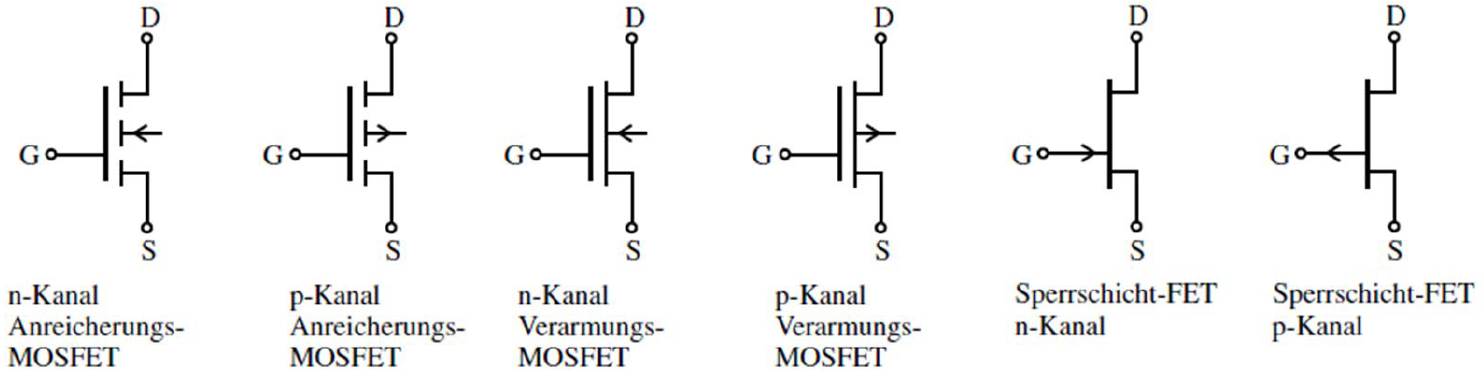
\includegraphics[align=t, width=\columnwidth]{images/fet_symbole_typen.png}


\subsubsection{Anschlüsse eines FET}

Kanal von \textbf{D}rain zu \textbf{S}ource (Stromfluss), gesteuert von \textbf{G}ate (und Bulk)


\subsection{Sperrschicht-FET / Junction FET (JFET)}

\subsubsection{Kennlinien}

\begin{minipage}[t]{0.43\columnwidth}
    \centering \textbf{Eingangskennlinie} \\
    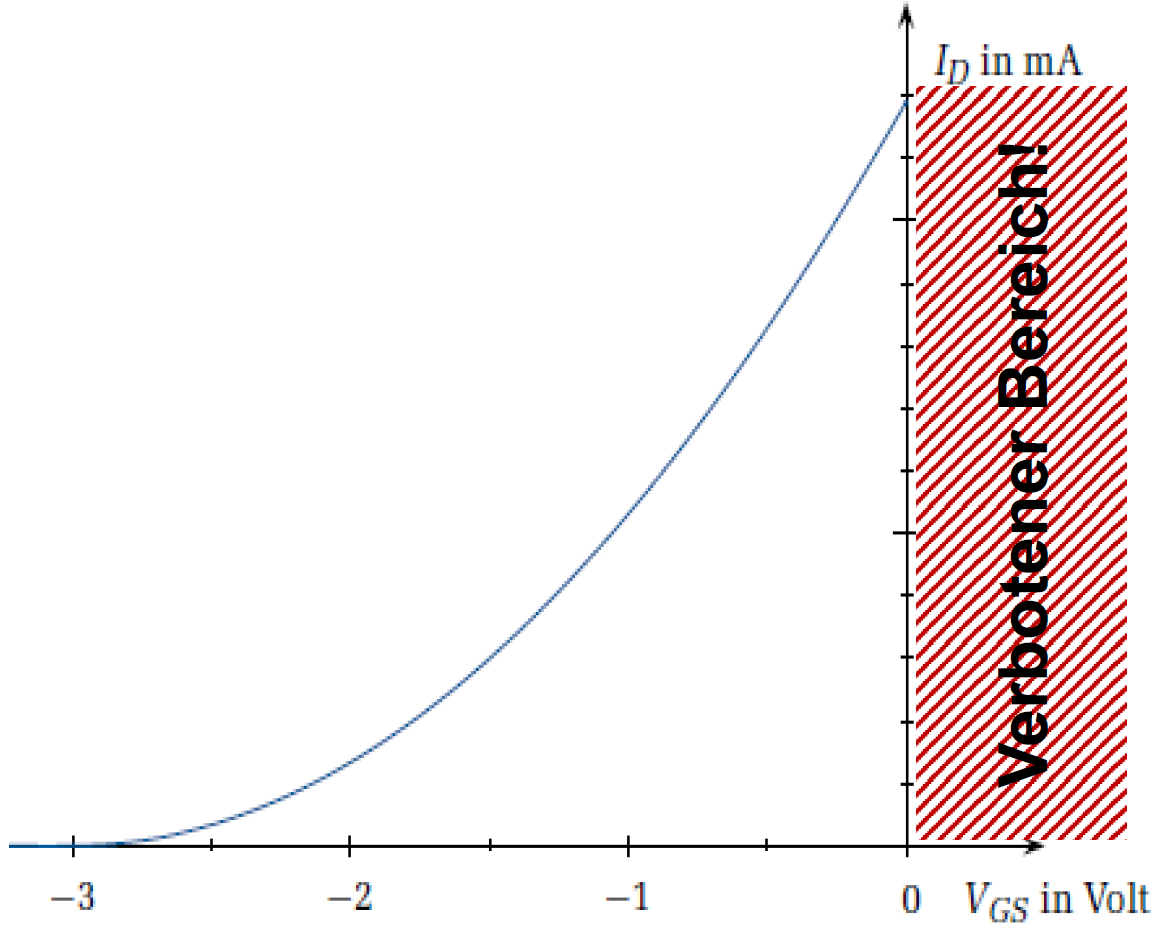
\includegraphics[align=c, width=\columnwidth]{images/jfet_eingangskennlinie.png}
\end{minipage}
\hfill
\begin{minipage}[t]{0.54\columnwidth}
    \textbf{Ausgangskennlinien} \\
    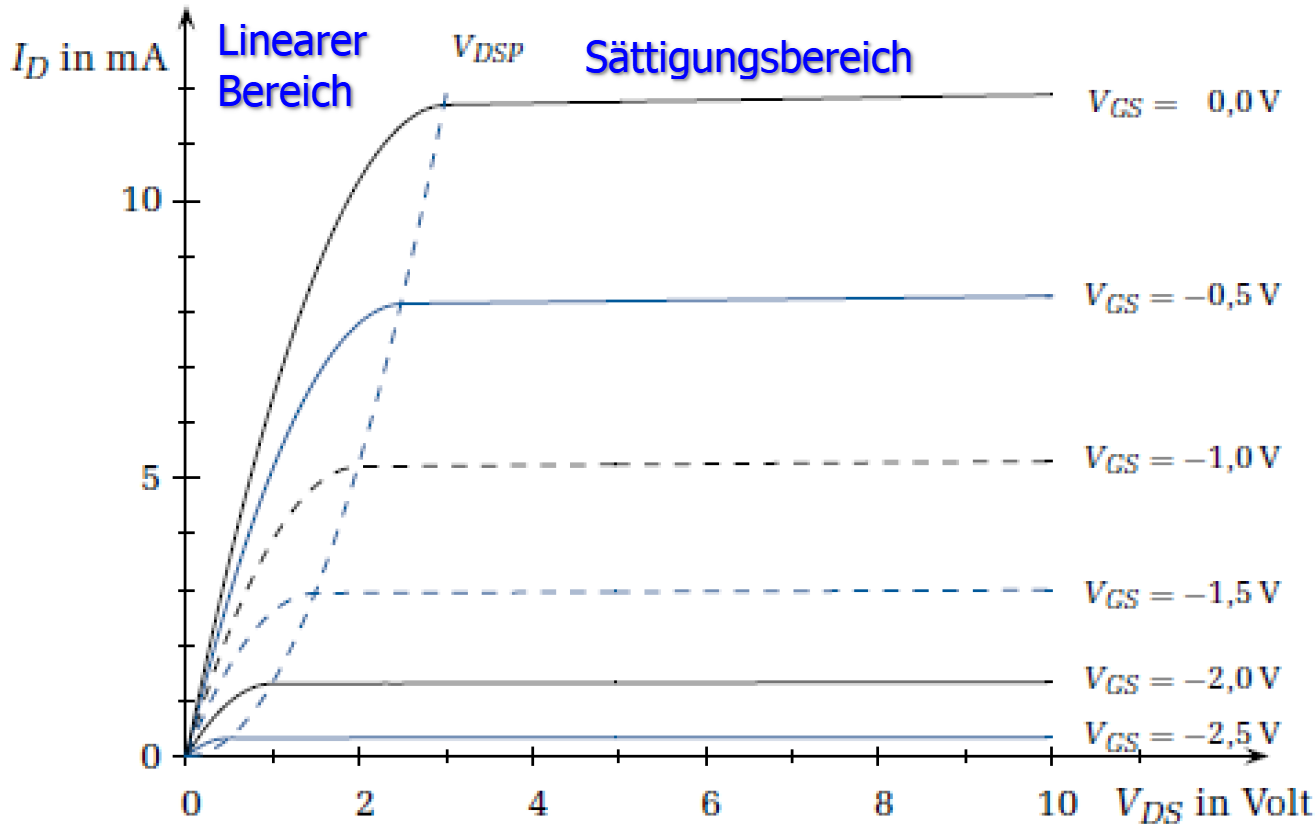
\includegraphics[align=c, width=\columnwidth]{images/jfet_ausgangskennlinien.png}
\end{minipage}


\subsubsection{Linearer Bereich (gesteuerter Widerstand)}

\begin{minipage}[t]{0.3\columnwidth}
    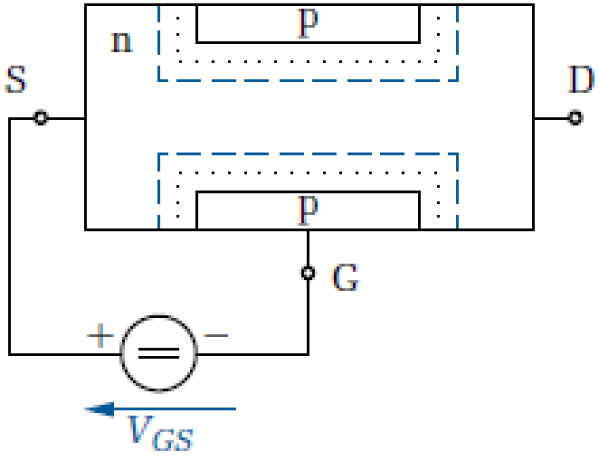
\includegraphics[align=t, width=\columnwidth]{images/fet_aufbau_linearer_bereich.png}
\end{minipage}
\hfill
\begin{minipage}[t]{0.68\columnwidth}
    \begin{itemize}
        \item Für \textbf{kleinen Spannung-Unterschied $V_{DS}$}
        \item $V_{GS}$ ändert Dicke der Raumladungszone (Kanal)
        \item n-Kanal JFET: Je negativer $V_{GS}$, desto weniger Strom fliesst bzw. desto enger der Kanal
    \end{itemize}

    $$ I_D = \frac{2 \cdot I_{DSS}}{V_p^2} \Big( V_{GS} - V_p - \frac{V_{DS}}{2} \Big) V_{DS} $$
\end{minipage}


\subsubsection{Sättigungs-Bereich (Stromquelle)}

\begin{minipage}[t]{0.3\columnwidth}
    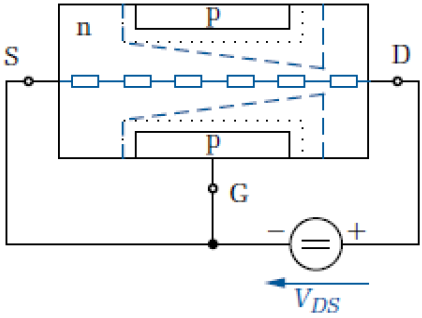
\includegraphics[align=t, width=\columnwidth]{images/fet_aufbau_saettigung.png}
\end{minipage}
\hfill
\begin{minipage}[t]{0.68\columnwidth}
    \begin{itemize}
        \item Für hohes $V_{DS}$ wird leitender Kanal abgeschürt \\
            \textrightarrow\ Strom kann nicht weiter steigen (Stromquelle)
        \item Übergang gest. Widerstand zu Stromquelle @ $V_{DSP}$ \\
        \textrightarrow\ $V_{DSP} = V_{GS} - V_p$ ($V_p =$ Pinch-Off-Spannung)
    \end{itemize}

    $$ I_D = \frac{ I_{DSS}}{V_p^2} \cdot ( V_{GS} - V_p )^2 $$
\end{minipage}

\vspace{0.2cm}
\textbf{Verstärkungsmass Transkonduktanz:}
$$ g_m = \frac{ 2 \cdot I_{DSS}}{V_p^2} \cdot ( V_{GS} - V_p ) = \frac{2}{| V_p |} \cdot \sqrt{I_{DSS} \cdot I_D} \qquad [g_m] = \siemens $$


\subsection{MOS-FETs}

\subsubsection{Aufbau}

\begin{minipage}[t]{0.35\columnwidth}
    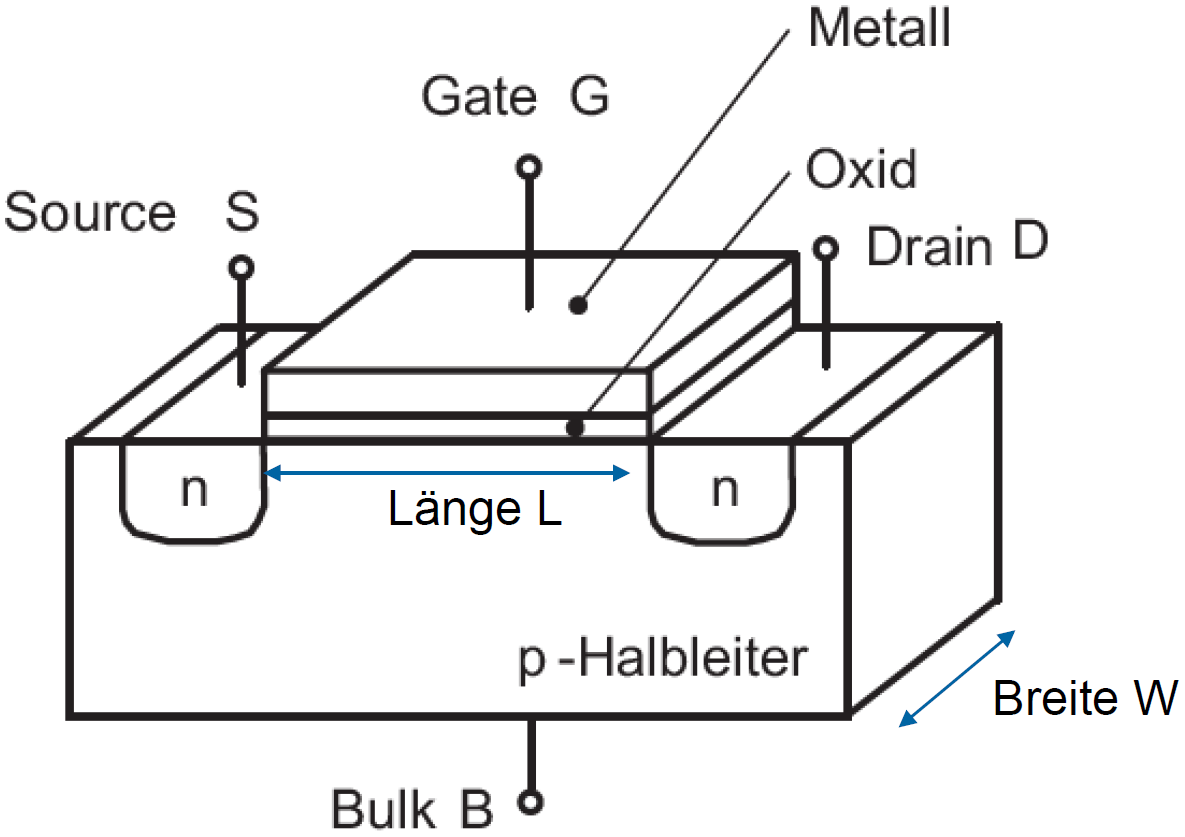
\includegraphics[align=c, width=\columnwidth]{images/mos_fet_aufbau.png}
\end{minipage}
\hfill
\begin{minipage}[c]{0.6\columnwidth}
    \begin{tabular}{l l}
        $L$ & Länge des Transistors  \\
        $W$ & Breite des Transistors \\
        \\
    \end{tabular}

    \begin{itemize}
        \item N-Kanal FET: Drain und Source sind n-dotiert
        \item Kanal ist p-dotiert
    \end{itemize}
\end{minipage}


\subsubsection{Kennlinien}

\begin{minipage}[t]{0.3\columnwidth}
    \textbf{Eingangskennlinie} \\
    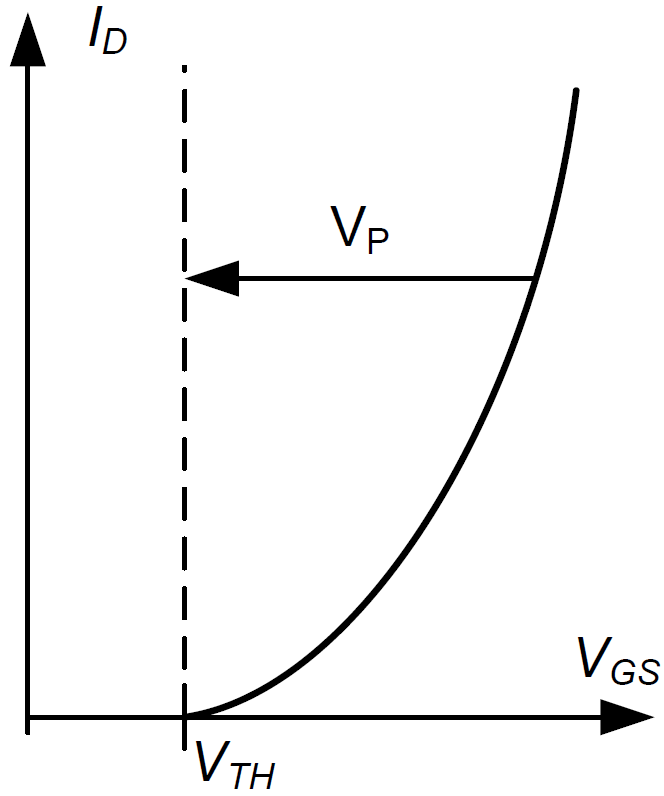
\includegraphics[align=c, width=\columnwidth]{images/mos_fet_eingangskennlinie.png}
\end{minipage}
\hfill
\begin{minipage}[t]{0.6\columnwidth}
    \textbf{Ausgangskennlinien} \\
    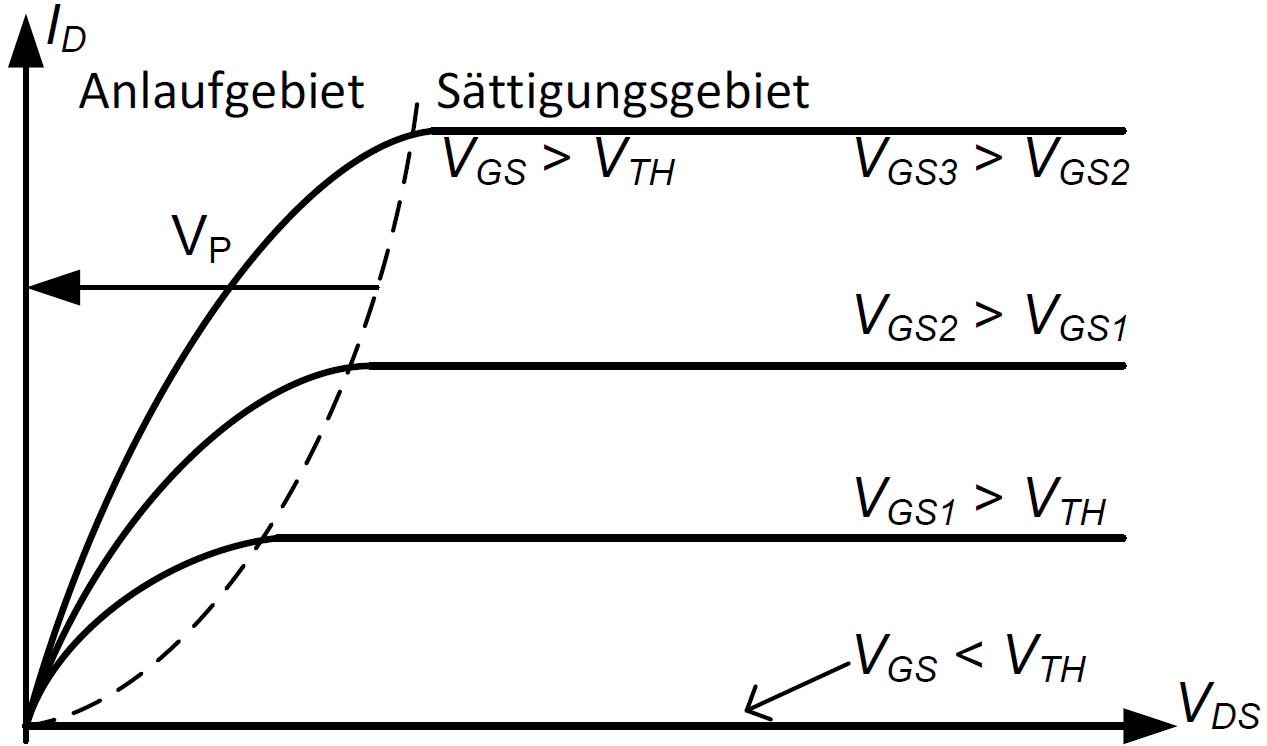
\includegraphics[align=c, width=\columnwidth]{images/mos_fet_ausgangskennlinien.png}
\end{minipage}


\subsubsection{Bereiche}

\begin{itemize}
    \item \textbf{Sperrbereich:} $V_{GS} < V_{TH}$ 
    \item \textbf{Linearer (Widerstands-)Bereich / Anlaufbereich:} $V_{GS} > V_{TH}$
    \item \textbf{Sättigungsbereich (Stromquelle):} $V_{DS} > V_{GS} - V_{TH}$
\end{itemize}

\vspace{0.2cm}

\begin{minipage}[t]{0.48\columnwidth}
    \textbf{Anlaufbereich (Linearer Bereich)}
    $$ I_{D,lin} = \beta \cdot ( V_{GS} - V_{TH} - \frac{V_{DS}}{2} ) \cdot V_{DS} $$
\end{minipage}
\hfill
\begin{minipage}[t]{0.48\columnwidth}
    \textbf{Sättigungsbereich (Stromquelle)}
    $$ I_{D,sat} = \frac{\beta}{2} \cdot ( V_{GS} - V_{TH} )^2 $$
\end{minipage}

% Kanallängenmodulation einfügen?


\subsubsection{Kleinsignal-Ersatzschaltung (MOS-FET)}

\begin{minipage}[t]{0.65\columnwidth}
    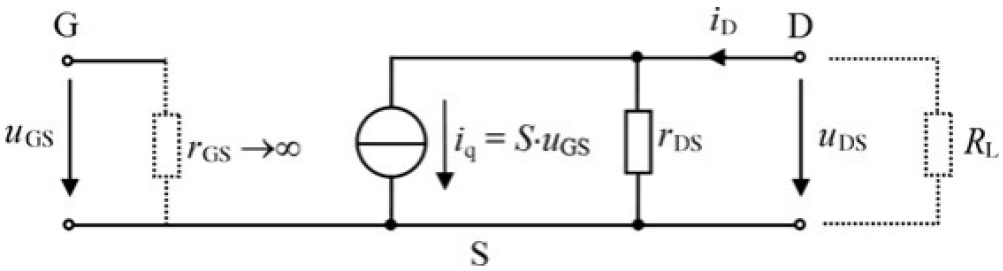
\includegraphics[align=t, width=\columnwidth]{images/mos_fet_kleinsignalersatzschaltung.png}
\end{minipage}
\hfill
\begin{minipage}[t]{0.33\columnwidth}
    $$ \beta = \frac{KP \cdot W}{L} $$
    $$ KP = C_{oc} \cdot \mu_n \approx 100 \frac{\micro \ampere}{\volt^2} $$  % kann man noch verbessern...
\end{minipage}

$$ S = g_m = \beta \cdot (V_{GS} - V_{TH}) = \sqrt{2 \cdot \beta \cdot I_D} = \sqrt{ 2 \cdot \frac{KP \cdot W}{L} \cdot I_D} $$
$$ \frac{1}{r_{DS}} = g_{DS} = \lambda \cdot I_D $$


\subsubsection{Temperaturabhängigkeit der Übrtragungskennlinie}

\begin{minipage}[c]{0.4\columnwidth}
    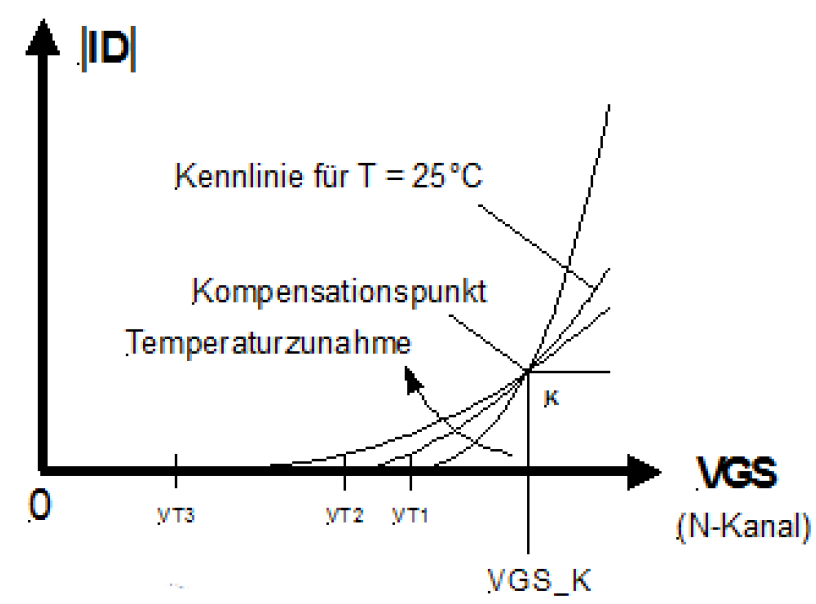
\includegraphics[width= \columnwidth]{images/mos_fet_eingangskennlinie_temperatur.png}
\end{minipage}
\hfill
\begin{minipage}[c]{0.58\columnwidth}
    Für den n-Kanal FET gilt:
    \begin{itemize}
        \item Threshold-Spannung $V_{TH}$ sinkt mit 1-2 $\frac{\micro \volt}{\kelvin}$
        \item $\beta$ sinkt mit steigender Temperatur
        \item Im Kompensationspunkt bleibt $I_D$ für fixes $V_{GS}$ konstant
    \end{itemize}
\end{minipage}

    
\subsection{Verstärkerschaltungen mit FETs}

\subsubsection{Source-Schaltung mit Lastwiderstand}

Um den Arbeitspunkt der Schaltung zu bestimmen, wird die \cbl{Lastgerade von $R_L$} in das
Ausgangskennlinienfeld eingezeichnet

\begin{minipage}[c]{0.4\columnwidth}
    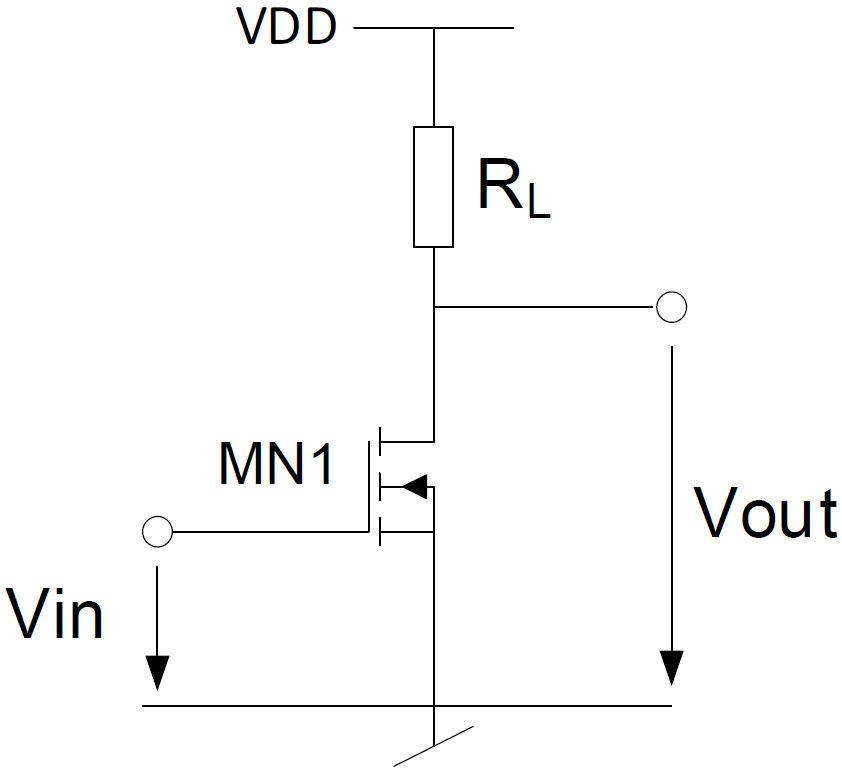
\includegraphics[width=0.9\columnwidth]{images/source_schaltung.png}
\end{minipage}
\hfill
\begin{minipage}[c]{0.5\columnwidth}
    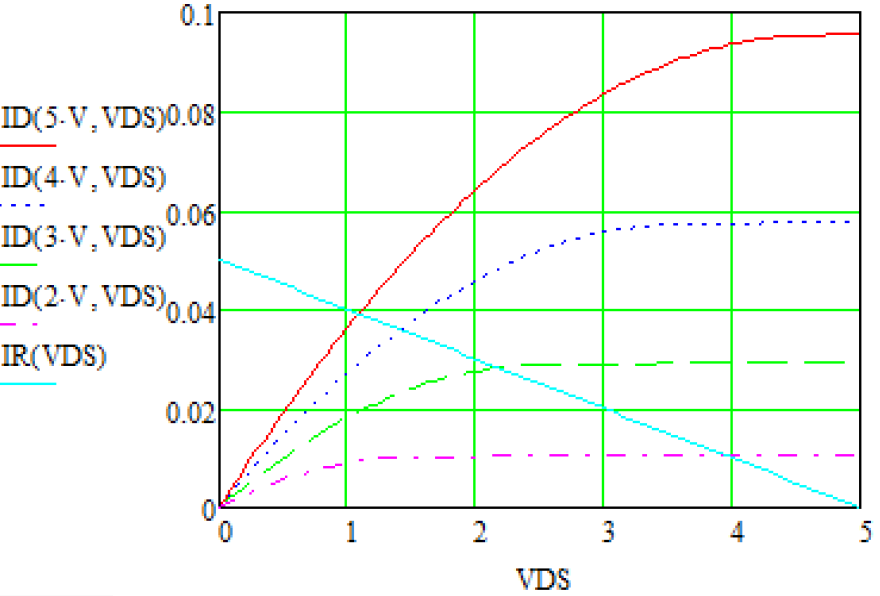
\includegraphics[width=\columnwidth]{images/source_schaltung_lastgerade.png}
\end{minipage}


\subsubsection{Push-Pull / Digitaler Inverter}  % eventuell weglassen

\begin{minipage}[c]{0.35\columnwidth}
    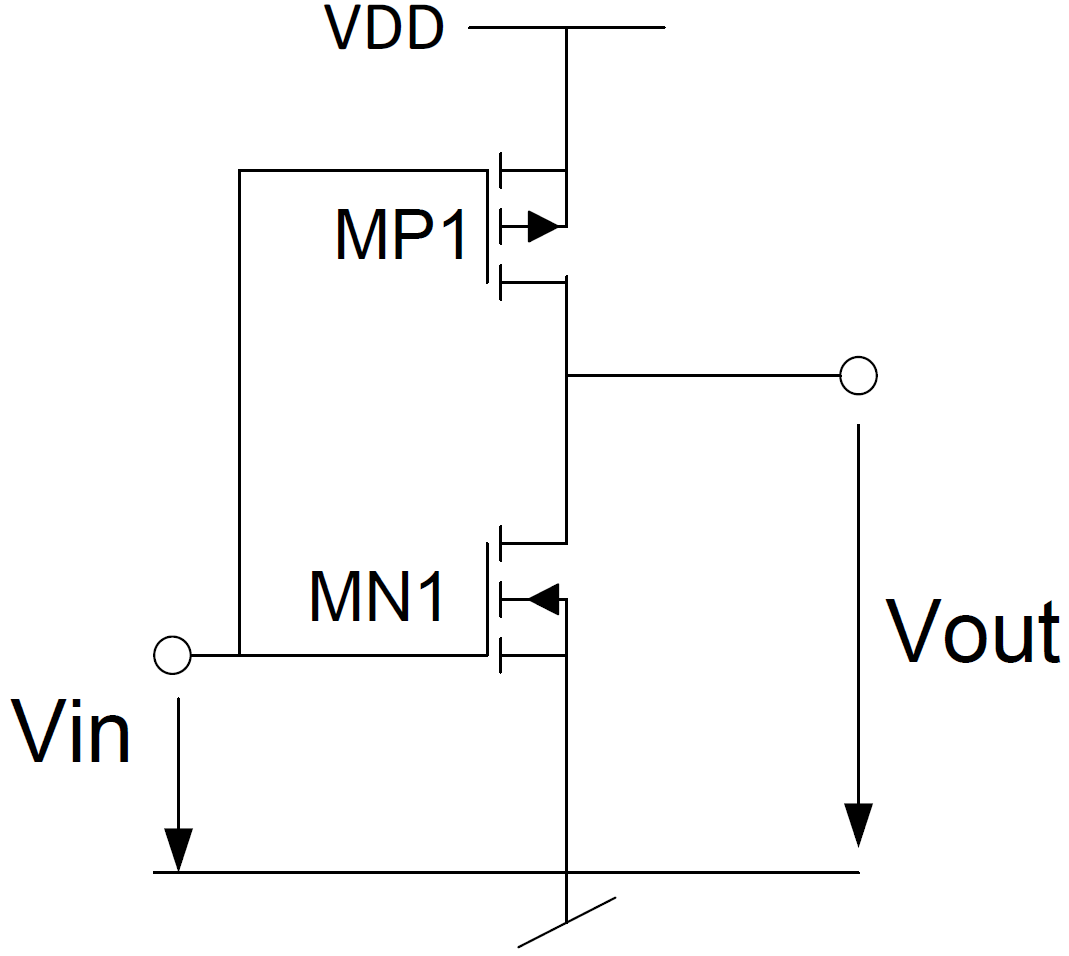
\includegraphics[width=\columnwidth]{images/push_pull_digital_inverter.png}
\end{minipage}
\hfill
\begin{minipage}[c]{0.5\columnwidth}
    \begin{itemize}
        \item $V_{in}$ geht auf NMOS und PMOS
        \item Ermöglicht grössere Verstärkung
    \end{itemize}
        
    \vspace{0.3cm}
    Für $V_{in} \approx \frac{V_{DD}}{2}$ gilt:
    $$ A_{V0} = -(g_{m1} + g_{m2}) \cdot (r_{DS1} || r_{DS2}) $$
\end{minipage}


\subsection{MOS-FET als (Leistungs-)Schalter}
Wenn der FET als Schalter eingesetzt wird, so arbeitet er im \textbf{linearen Bereich} \\
($V_{GS} > V_{TH}$, d.h. $V_{out} < V_{DD} - V_{TH} $)

\begin{minipage}[c]{0.49\columnwidth}
    $$ I_{D,lin} = \beta \cdot ( V_{GS} - V_{TH} - \frac{V_{DS}}{2} ) \cdot V_{DS} $$
    \begin{center}
        
        Schalter geschlossen: $R_{FET} = R_{DS(on)} $
    \end{center}
\end{minipage}
\hfill
\begin{minipage}[c]{0.49\columnwidth}
    $$ r_{DS} = \dfrac{\diff V_{DS}}{\diff I_D} = \frac{1}{\beta \cdot (V_{GS} - V_{TH})}  $$
    \begin{center}
        Schalter offen: $R_{FET} = \infty$ 
    \end{center}
\end{minipage}


\subsubsection{Verlustleistung / Erwärmung}

\begin{minipage}[c]{0.48\columnwidth}
    $$ P_V = R_{DS} * I_{DS}^2 = 0 \, \watt $$
\end{minipage}
\hfill
\begin{minipage}[c]{0.48\columnwidth}
    $$ \Delta T = R_{th} \cdot P_V $$
\end{minipage}


\subsection{Transmission Gate}

\begin{minipage}[c]{0.22\columnwidth}
    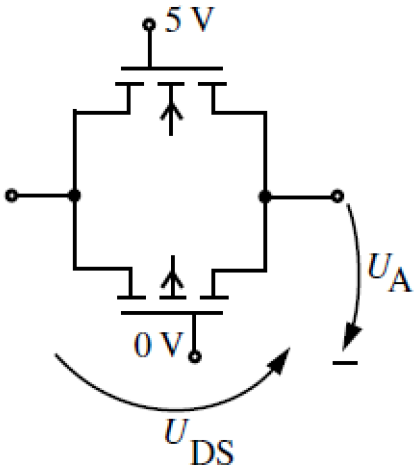
\includegraphics[width=\columnwidth]{images/transmission_gate.png}
\end{minipage}
\hfill
\begin{minipage}[c]{0.68\columnwidth}
    Im Bild links gilt: $V_{DD} = 5 \, \volt$, $V_{SS} = 0 \, \volt$ 

    \begin{itemize}
        \item NMOS (oben) leitet für $V_{in} < V_{DD} - T_{TH,n}$
        \item PMOS (unten) leitet für $V_{in} > V_{SS} - T_{TH,p}$
        \item Source und Drain austauschbar \\
            \textrightarrow\ Strom kann in beide Richtungen fliessen
    \end{itemize}
\end{minipage}
        \section{Transistor-Transistor-Logik}

\begin{itemize}
    \item Meist statischer Stromverbrauch
    \item Asymmetrische Schaltschwellen (weniger Marge als CMOS-Logik)
\end{itemize}


\subsection{Resistor Transistor Logik (RTL)}

\begin{minipage}[c]{0.27\columnwidth}
    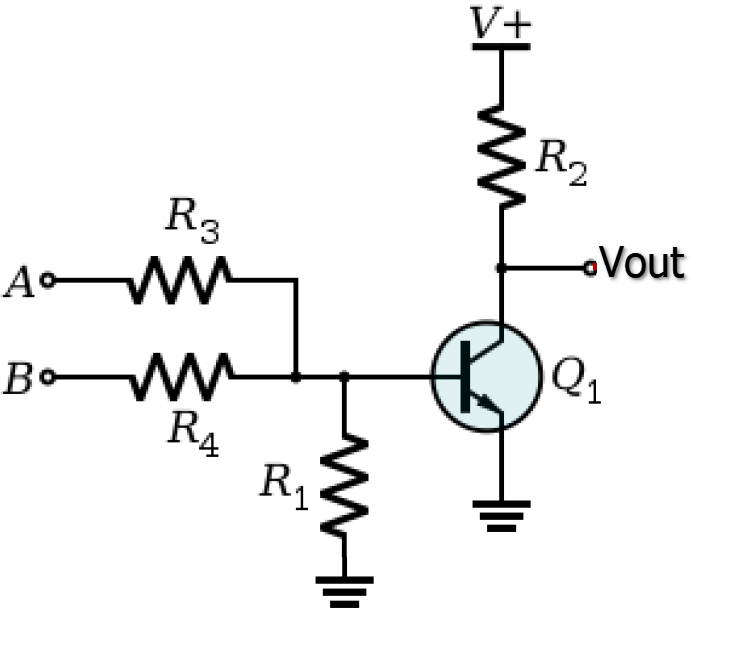
\includegraphics[width=\columnwidth]{images/rtl_nor.png}
\end{minipage}
\hfill
\begin{minipage}[c]{0.68\columnwidth}
    Bild: NOR-Gate

    \begin{itemize}
        \item Ausgangsspannung $V_{out} = V_+$ oder $V_{out} = V_{CE,sat}$
        \item \textbf{Fan-Out ist begrenzt} (Werden zu viele weitere Gatter an den Ausgang gehängt, so reicht der Strom nicht mehr,
             um diese zu treiben \textrightarrow Spannungslevel stimmen nicht mehr, um Transisoren durchzusteuern)
    \end{itemize}
\end{minipage}


\subsection{Dioden-Transistor-Logik (DTL)}

\begin{minipage}[c]{0.3\columnwidth}
    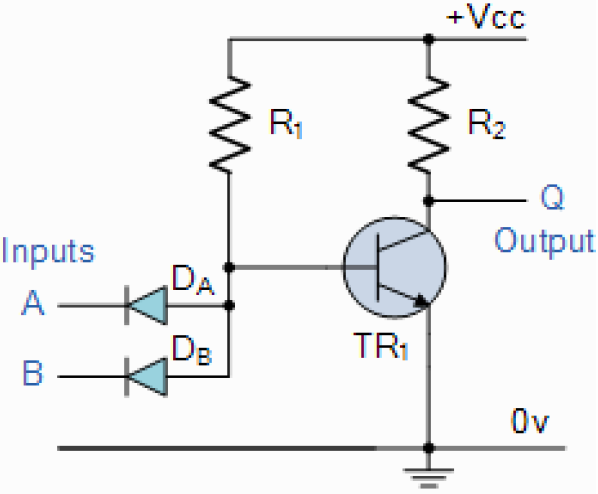
\includegraphics[width=\columnwidth]{images/dtl_nand_gate.png}
\end{minipage}
\hfill
\begin{minipage}[c]{0.68\columnwidth}
    Bild: NAND-Gate

    \begin{itemize}
        \item \textbf{Fan-Out grösser}, da Transistor aktiv nach '0' zieht
        \item $R_2$ muss keine Gatter treiben (kein grosser Stromfluss)
        \item Nachteile: Sehr tiefer Störabstand; Transistor leitet schon bei Spannungen, welche kaum $> 0 \, \volt$ sind 
    \end{itemize}
\end{minipage}


\subsection{Transistor-Transistor-Logik (TTL)}

\begin{minipage}[c]{0.3\columnwidth}
    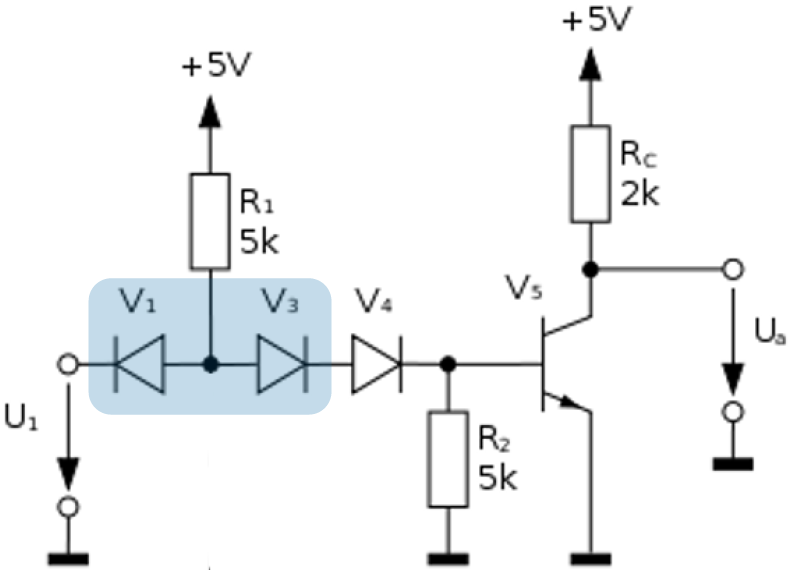
\includegraphics[width=\columnwidth]{images/dtl_zu_ttl.png}
\end{minipage}
\hfill
\begin{minipage}[c]{0.15\columnwidth}
    % better image: will be done by A.K.
    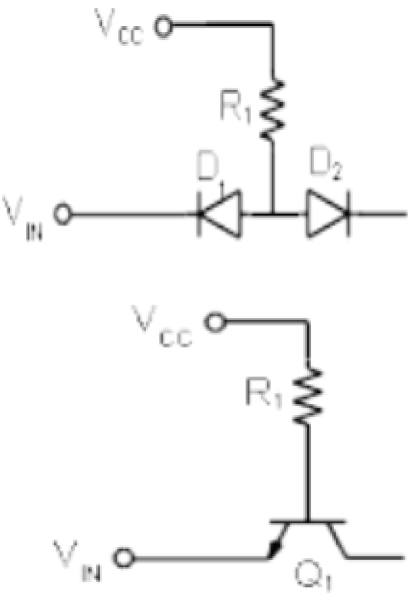
\includegraphics[width=\columnwidth]{images/dtl_zu_ttl_transistors.png}
\end{minipage}
\hfill
\begin{minipage}[c]{0.48\columnwidth}
    \begin{itemize}
        \item  Schaltschwelle am Eingang wird durch Dioden $V_3$ und $V_4$ um $1.4 \, \volt$ erhöht
        \item Dioden $V_1$ und $V_2$ bilden npn-Struktur \textrightarrow npn-Transistor
    \end{itemize}
\end{minipage}


        \section{CMOS-Logik}

\begin{itemize}
    \item Entweder leitender Pfad nach $V_{\rm SS}$ (NMOS) oder $V_{\rm DD}$ (PMOS)
    \item Kein statischer Stromverbrauch
    \item Langsamer als Bipolar
    \item Symmetrische Schaltschwellen bei ca. $\frac{V_{\rm DD}}{2}$ (Übertragungskennlinie)
    \item Output-Level $V_{\rm ol}$, $V_{\rm oh}$ näher bei Speisung als Input Level $V_{\rm il}$, $V_{\rm ih}$ \textrightarrow\ mehr Marge
    \item Höhere Speisespannung \textrightarrow\ weniger propagation delay
    \item Nicht geeignet zur Datenübertragung über längere Strecken (kein $50 \, \ohm$ Abschluss)
\end{itemize}


\subsection{Grundgatter in CMOS-Logik}

\begin{minipage}[t]{0.32\columnwidth}
    \begin{center}
        \textbf{Inverter} \\
        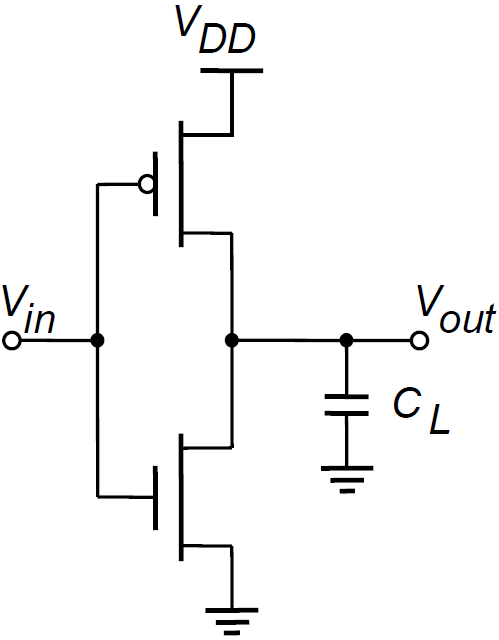
\includegraphics[width=\columnwidth]{images/cmos_inverter.png}
    \end{center}
\end{minipage}
\hfill
\begin{minipage}[t]{0.27\columnwidth}
    \begin{center}
        \textbf{NAND-Gate} \\
        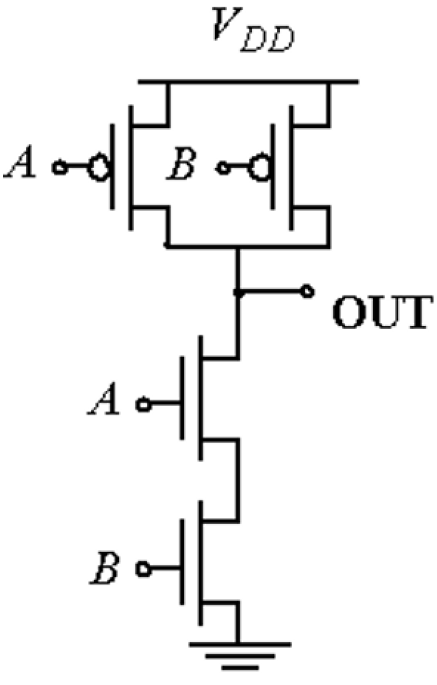
\includegraphics[width=\columnwidth]{images/cmos_nand_2.png}
    \end{center}
\end{minipage}
\hfill
\begin{minipage}[t]{0.38\columnwidth}
    \begin{center}
        \textbf{NOR-Gate} \\
        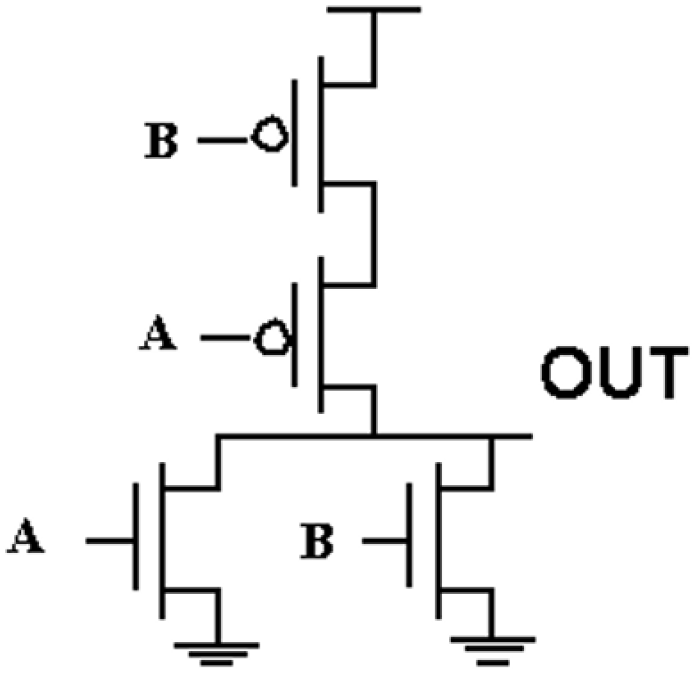
\includegraphics[width=\columnwidth]{images/cmos_nor.png}
    \end{center}
\end{minipage}


\subsection{Dualität NMOS -- PMOS}

\begin{minipage}[c]{0.45\columnwidth}
    \begin{center}
        \textbf{PMOS} \\
        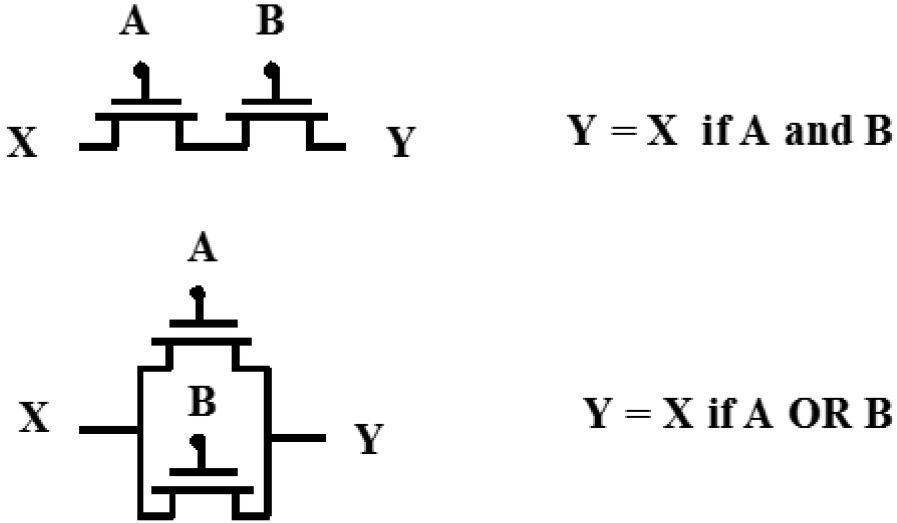
\includegraphics[width=\columnwidth]{images/nmos_dualitaet.png}
    \end{center}
\end{minipage}
\hfill
\begin{minipage}[c]{0.45\columnwidth}
    \begin{center}
        \textbf{NMOS} \\
        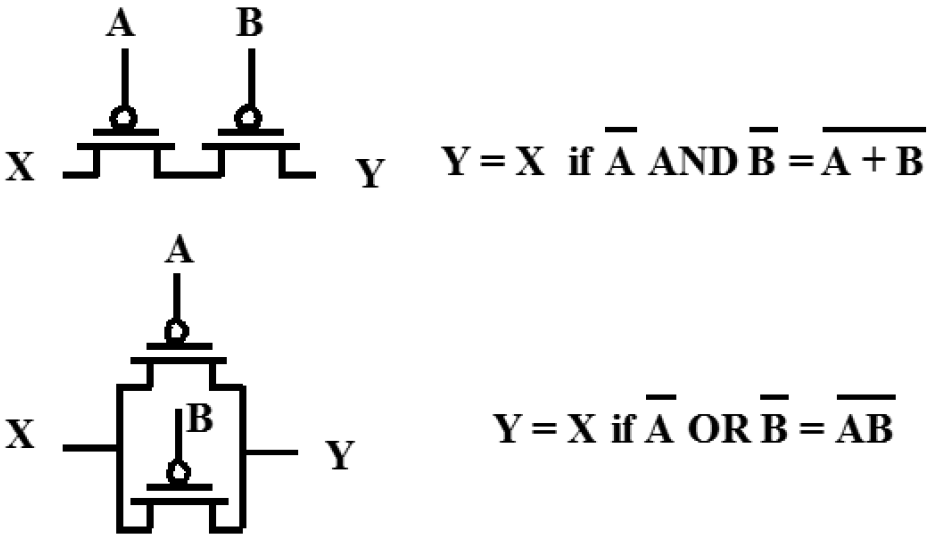
\includegraphics[width=\columnwidth]{images/pmos_dualitaet.png}
    \end{center}
\end{minipage}


\subsection{Verlustleistung bei CMOS-Logik}

\begin{minipage}[c]{0.48\columnwidth}
    $$ \boxed{ P_V = C \cdot V_{\rm CC}^2 \cdot f} $$
\end{minipage}
\hfill
\begin{minipage}[c]{0.48\columnwidth}
    \begin{tabular}{ll}
        $C$ & Kapazität (aus Datenblatt) \\
        $f$ & Frequenz 
    \end{tabular}
\end{minipage}


\subsection{Verzögerungszeit}

\begin{minipage}[t]{0.48\columnwidth}
    \textbf{Linearer Bereich}
    $$ \boxed{t_{\rm pHL} = 0.69 \cdot R_{\rm on} \cdot C_L} $$
    \textrightarrow\ Exponentielle Entladung! 
\end{minipage}
\hfill
\begin{minipage}[t]{0.48\columnwidth}
    \textbf{Sättigung (Stromquellen-Bereich)}
    $$ \boxed{t_{\rm pHL} = \frac{C_L \cdot \frac{V_{\rm swing}}{2}}{I_{\rm sat}} \approx \frac{C_L}{k_n \cdot V_{\rm DD}} }$$
    \textrightarrow\ Lineare Entladung!
\end{minipage}


% TODO: Kennlinien / Charakteristik CMOS-Technologie...?
% \section{CMOS  vs. TTL Logikpegel}
% 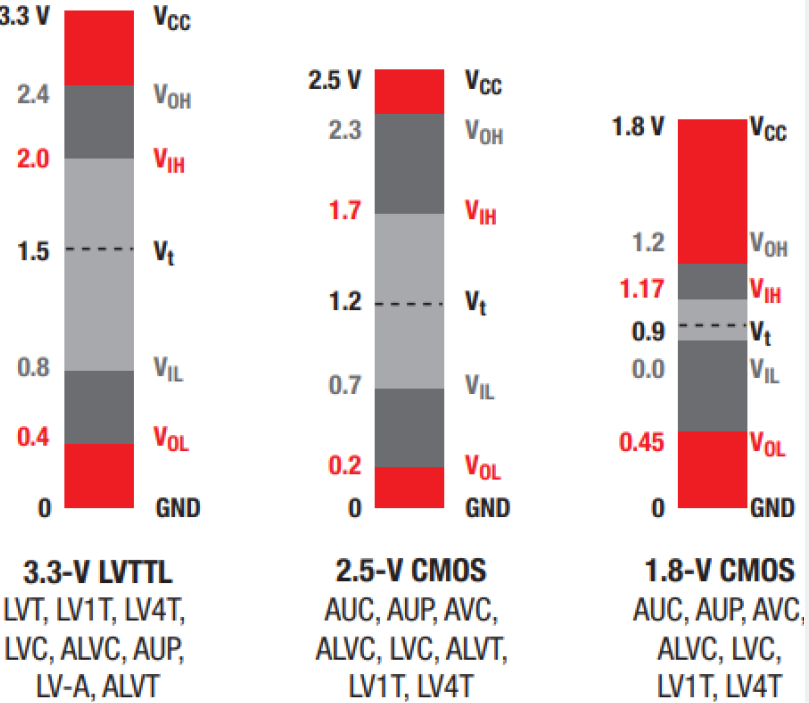
\includegraphics[width=0.75\columnwidth]{images/logik_pegel.png}
        \section{Schmitt-Trigger}

\begin{itemize}
    \item Schaltschwellen müssen nicht sehr genau sein
    \item Schmitt-Trigger garantieren auch bei verrauschten Signalen saubere (einmalige) Schaltschwellen, dank der Hysterese
\end{itemize}



\subsection{Aufbau nichtinvertierender digitaler Schmitt-Trigger}

\begin{minipage}[position]{0.35\columnwidth}
    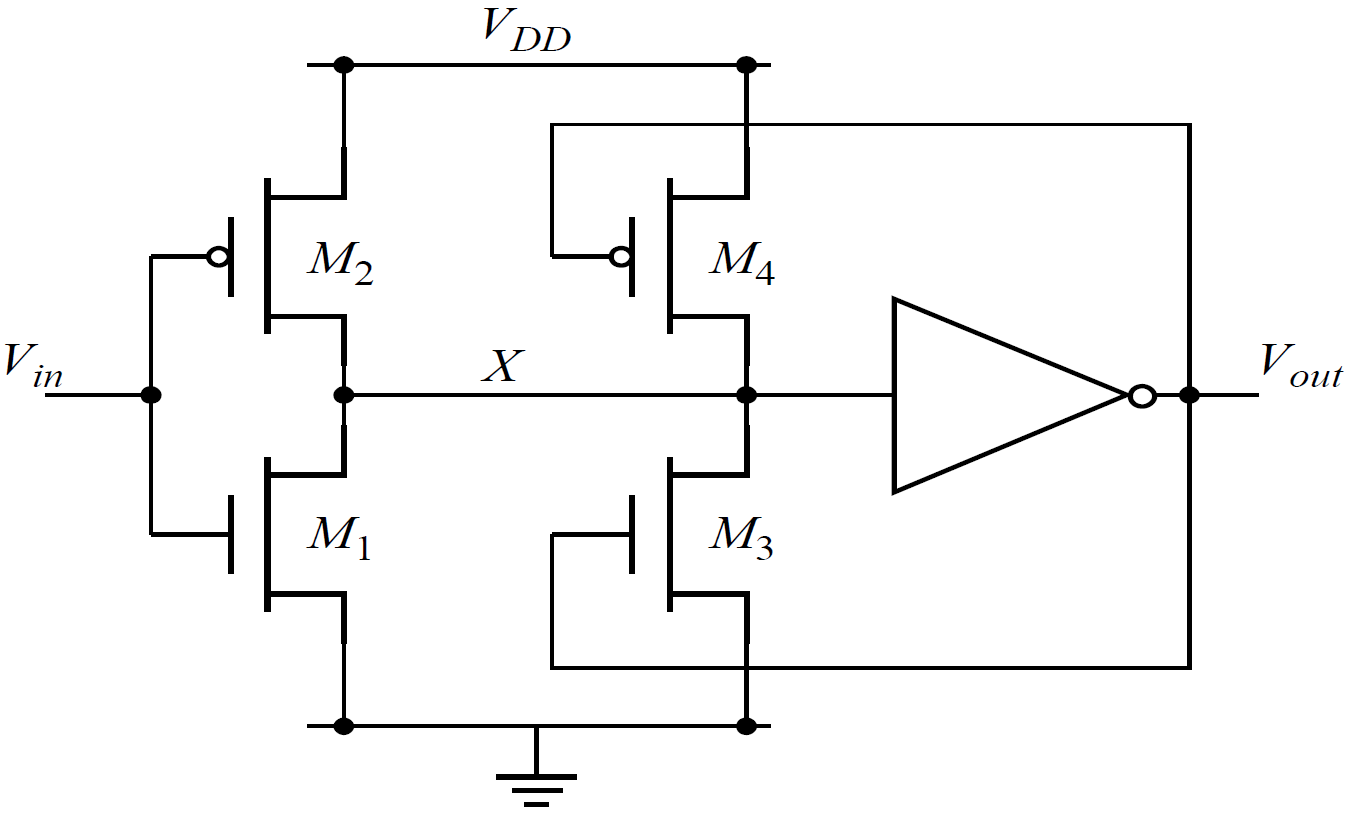
\includegraphics[width=\columnwidth]{images/nichtinvertierender_schmitt-trigger.png}
\end{minipage}
\hfill
\begin{minipage}[position]{0.63\columnwidth}
    \begin{itemize}
        \item $M_1, M_2$: Digitale Inverter
        \item $M_3, M_4$: gesteuerte Widerstände
        \item \textbf{Für }$\boldsymbol{V_{\rm out} = 0}$: $M_4$ leitet, $M_3$ sperrt
        \item \textbf{Für }$\boldsymbol{V_{\rm out} = 1}$: $M_3$ leitet, $M_4$ sperrt
        \item $M_3, M_4$ verschieben Schaltschwellen abhängig von $V_{\rm out}$ \textrightarrow\ Hysterese
    \end{itemize}
\end{minipage}


\subsection{Aufbau invertierender digitaler Schmitt-Trigger}

\begin{minipage}[position]{0.3\columnwidth}
    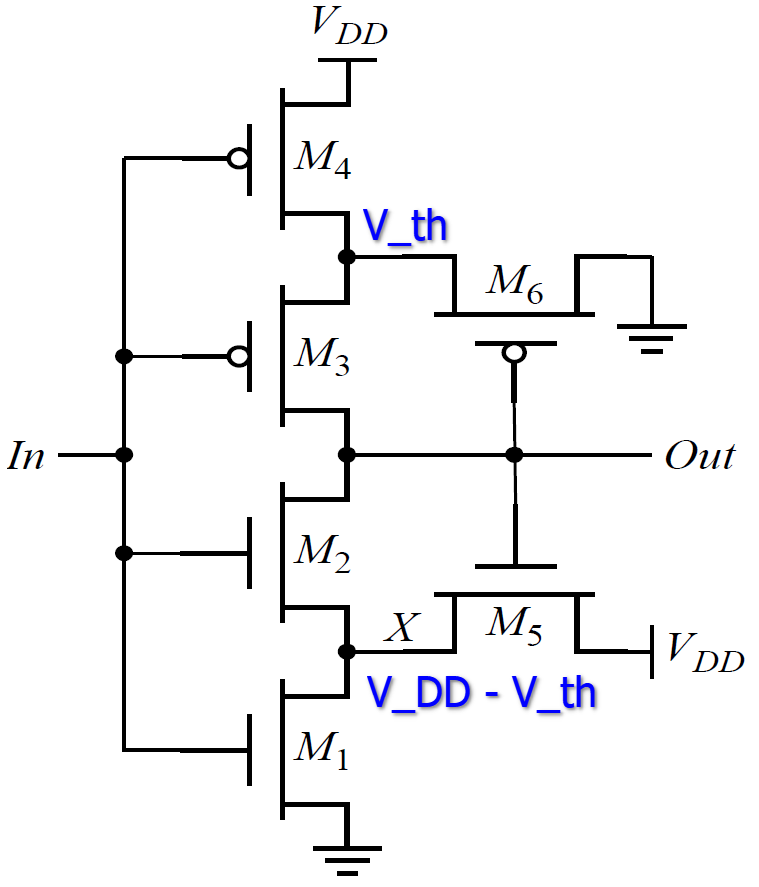
\includegraphics[width=\columnwidth]{images/invertierender_schmitt-trigger.png}
\end{minipage}
\hfill
\begin{minipage}[position]{0.68\columnwidth}
    \begin{itemize}
        \item Ohne $M_5, M_6$: Normaler Inverter mit je 2\\
            Serie-Transistoren
        \item \textbf{Für }$\boldsymbol{V_{\rm out} = 1}$: Durch $M_5$ fliesst Strom in $M_1$
        \item $V_{\rm in}$ muss höher sein, um Strom der PMOS aufzunehmen\\
            \textrightarrow\ Höhere Schaltschwelle für High-Low-Übergang
        \item 'Inverses' gilt für $M_6$ und $M_4$
    \end{itemize}
\end{minipage}


\subsection{Schmitt-Trigger vs. CMOS-Logik}

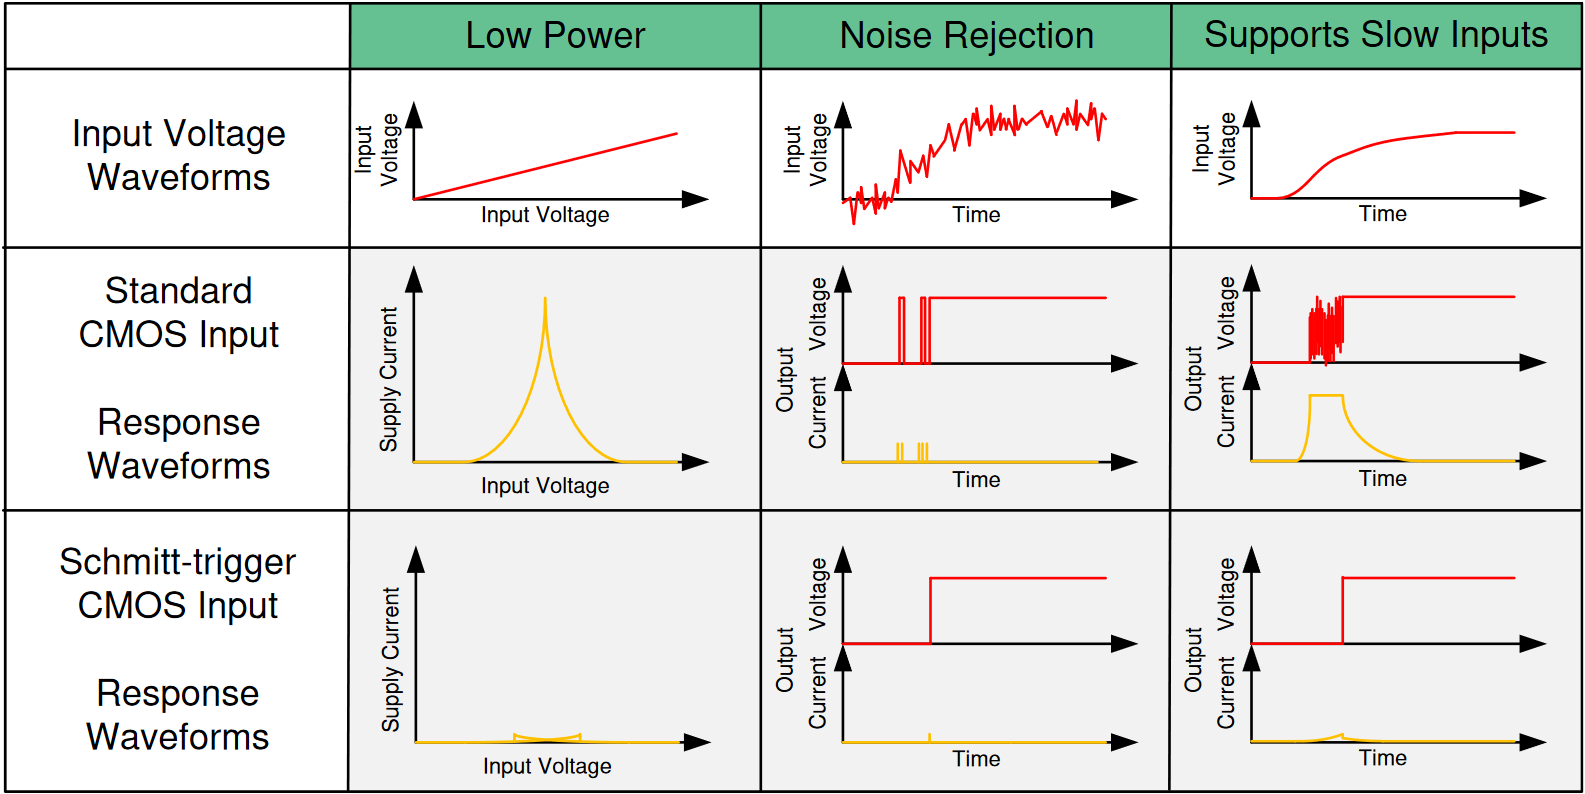
\includegraphics[width=\columnwidth]{images/benefits_schmitt-trigger.png}


        \section{Signalübertragung}

\subsection{Leitungstheorie}

\begin{itemize}
    \item Leitungen haben Widerstände, Kapazitäten und Induktivitäten \textrightarrow\ RLC-Netzwerke
    \item \textbf{Fortpflanzungsgeschwindigkeit Signal:} $v = 10 - 20 \, \centi \meter / \nano \second$ \\
        (Lichtgeschwindigkeit: $c = 0 \, \centi \meter / \nano \second$) % TODO: 0 correct?
    \item Ev. \textbf{Impedanzanpassungen} zur Verhinderung von \textbf{Reflexionen} nötig (meistens $50 \, \ohm$)
    \item CMOS-Logik: tiefen Quellenwiderstand, hohen Eingangswiderstand \\
        \textrightarrow\ Nicht geeignet zur Datenübertragung über 'längere Strecken'
\end{itemize}


\subsection{Einfluss / Relevanz von Refelxionen}

\subsubsection{Keine Reflexionen}

Wenn nichts anderes bekannt gilt: $T_r = \frac{1}{10} \cdot T$ 

\begin{minipage}[c]{0.3\columnwidth}
    $$ \boxed{ T_d < \frac{1}{2} \cdot T_r} $$
\end{minipage}
\hfill
\begin{minipage}[c]{0.68\columnwidth}
    \begin{tabular}{ll}
        $T_r = T_f$ & Anstiegs- / bzw. Abfallzeit des Signals \\
        $T_d$       & Laufzeit des Signals \\
        $T$         & Periodendauer
    \end{tabular}
\end{minipage}


\subsubsection{Reflexionen}

\begin{minipage}[c]{0.3\columnwidth}
    $$ \boxed{ l > \frac{1 \cdot 10^7 \, \frac{\meter}{\second} }{f_{\rm max}} } $$
\end{minipage}\hfill
\begin{minipage}[c]{0.68\columnwidth}
    \begin{tabular}{ll}
        $f_{\rm max}$   & Maximal enthaltene Frequenz im Signal \\
        $l$         & Länge der Leitung 
    \end{tabular}
\end{minipage}


        \section{High-Speed-Logik}

\begin{itemize}
    \item Sättigung verhindern, da langsam (bei Bipolar-Transistoren)
    \item Reduzierter Spannungshub
    \item Stromsteuerung, da Ströme schneller geschaltet werden als Spannungen
\end{itemize}


\subsection{Emitter Coupled Logic (ECL)}

\subsubsection{Emitter Coupled Logic (ECL)}

\begin{minipage}[c]{0.3\columnwidth}
    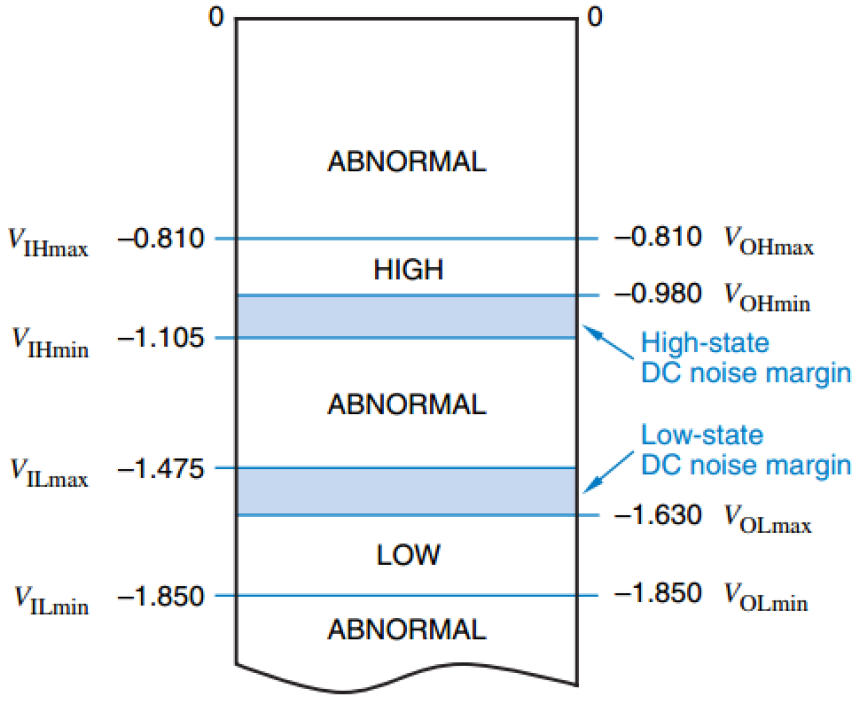
\includegraphics[width=\columnwidth]{images/ECL_logikpegel.png}
\end{minipage}
\hfill
\begin{minipage}[c]{0.68\columnwidth}
    \begin{itemize}
        \item 2 Familien: $10 \kilo$ (langsamer) und $100 \kilo$ (schneller)
        \item Positive Speisung: $V_{CC} = 0 \, \volt$
        \item Negative Speisung: $V_{EE} = -4.5 \, \volt$ / $V_{EE} = -5.2 \, \volt$ 
        \item ICs werden warm ($40 \, \milli \watt$ pro Gatter)
    \end{itemize}
\end{minipage}

\begin{minipage}[c]{0.25\columnwidth}
    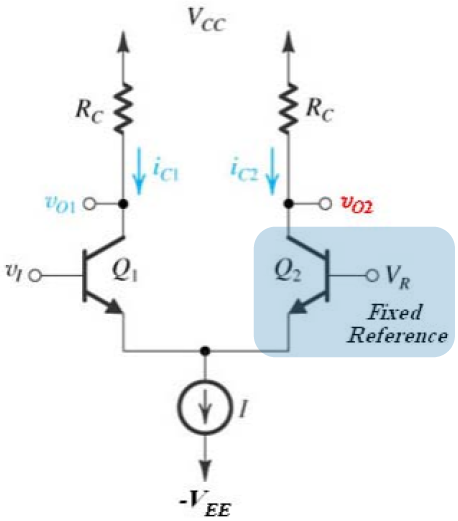
\includegraphics[width=\columnwidth]{images/ECL.png}
\end{minipage}
\hfill
\begin{minipage}[c]{0.72\columnwidth}
   \begin{itemize}
    \item Eingangssignal $V_I$ wird mit fixer Referenz $V_R$ verglichen
    \item Von $V_R - 100 \, \milli \volt$ bis $V_R + 100 \, \milli \volt$ \textbf{kippt Ausgnagsspannung} von 
        $V_{CC}$ auf $V_{CC} - R_C \cdot I_C$
    \item \textbf{Differentieller Spannungshub} der Ausgänge: \\
        $V_{diff} = \pm R_C \cdot I_C$
    \item Spannungspegel \textbf{nicht} kompatibel zu CMOS / TTL
   \end{itemize}
\end{minipage}


\subsubsection{Positive Emitter Coupled Logic PECL}

\begin{minipage}[c]{0.25\columnwidth}
    % Bild ist eventuell zu klein -> Testdruck machen
    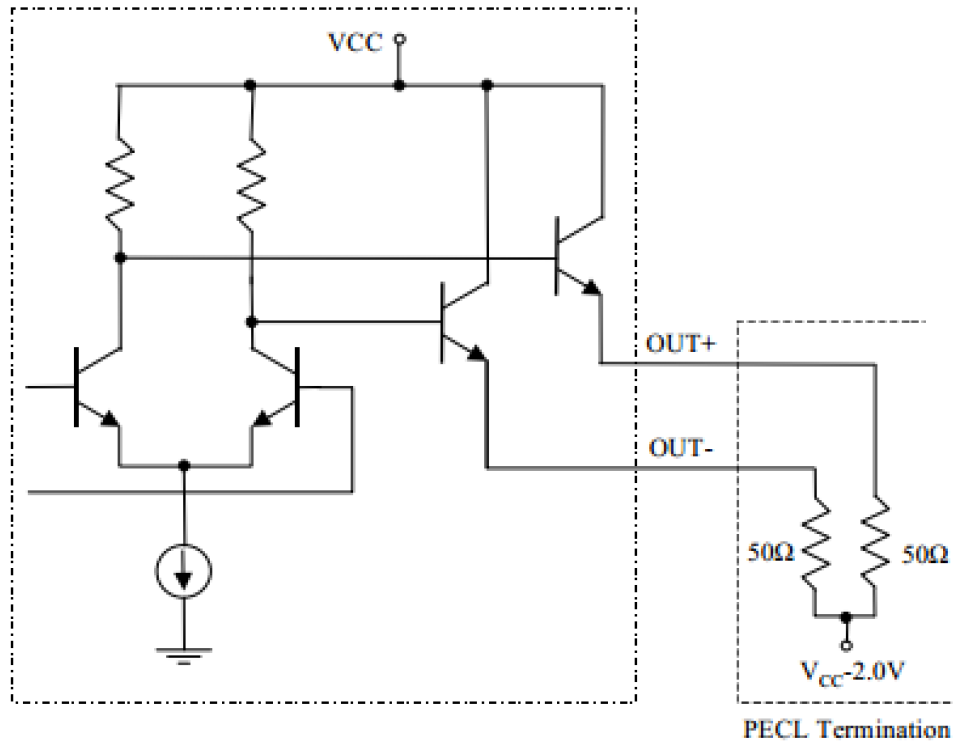
\includegraphics[width=\columnwidth]{images/PECL.png}
\end{minipage}
\hfill
\begin{minipage}[c]{0.72\columnwidth}
   \begin{itemize}
    \item Positive Speisung: $V_{CC} = 5 \, \volt$
    \item Negative Speisung: $V_{EE} = 0 \, \volt$
    \item Ausgangsbeschaltung mit $50 \, \ohm$ Abschluss zu $V_{CC} - 2 \, \volt$ \\
        \textrightarrow\ Reduktion der Reflexionen!
    \item Spannungspegel sind kompatibel zu CMOS / TTL
   \end{itemize}
\end{minipage}

% falls zu wenig Platz, diese subsubsection weglassen
\subsubsection{Low Voltage Positive ECL (LVPECL)}

\begin{itemize}
    \item Speisespannungen:  $V_{CC} = 3.3 \, \volt$; $V_{EE} = 0 \, \volt$
    \item Weniger Leisutng als $5 \, \volt$ Logik; leichter anpassbar an $3.3 \, \volt$ Logik
\end{itemize}


\subsection{Current Mode Logic (CML)}

\begin{minipage}[c]{0.25\columnwidth}
    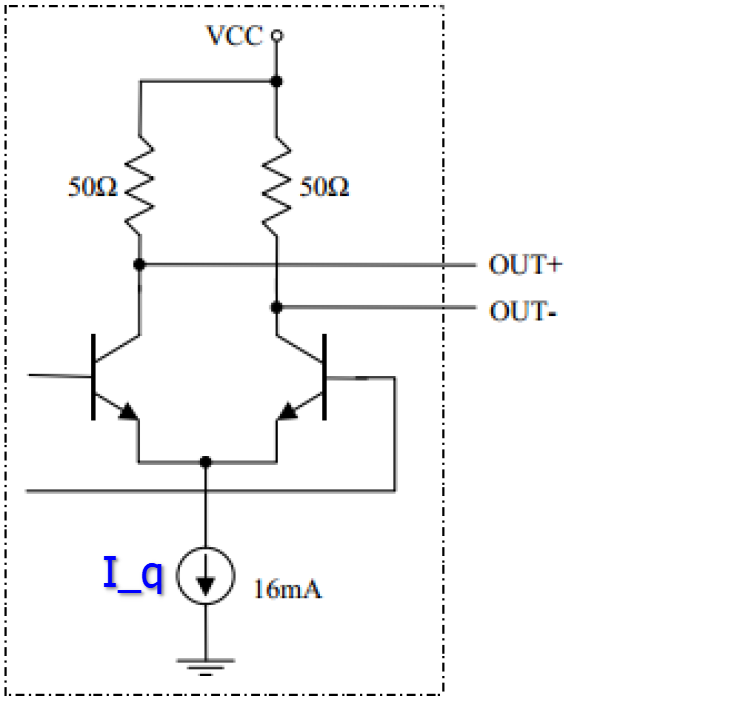
\includegraphics[width=\columnwidth]{images/CML.png}
\end{minipage}
\hfill
\begin{minipage}[c]{0.72\columnwidth}
   \begin{itemize}
    \item Terminierung am Eingang der Folgestufe gegen $V_{CC}$
    \item Äquivalenter Widerstand: $R_{C_{eq}} = 50 \, \ohm \, || \, 50 \, \ohm = 25 \, \ohm$
    
    $$ \boxed{ \text{Differentielle Spannung: } V_{diff} = \pm R_{C_{eq}} \cdot I_q }$$
   \end{itemize}
\end{minipage}


\subsubsection{CML vs. ECL}

\begin{minipage}[t]{0.55\columnwidth}
    \begin{center}
        \textbf{ECL}
    \end{center}

    \begin{itemize}
        \item Diff-Amp mit Transistor-Bufffer; Ausgang am Emitter 
        \item Single-ended Input (2. Eingang auf fixer Spannung)
        \item Single-ended Output (z.T. auch differentiell)
    \end{itemize}
\end{minipage}
\hfill
\begin{minipage}[t]{0.43\columnwidth}
    \begin{center}
        \textbf{CML}
    \end{center}

    \begin{itemize}
        \item Ausgang direkt vom Diff-Amp
        \item Differentieller Input und differentieller Output
        \item Impedanzanpassung zur Reduktion von Reflexionen ($50 \, \ohm$)
    \end{itemize}
\end{minipage}


\subsubsection{Vorteile / Nachteile von CML gegenüber CMOS-Logik}

\begin{minipage}[t]{0.48\columnwidth}
    \raggedcolumns
    \begin{itemize}
        \item[+] high Speed
        \item[+] konstanter Strom (kaum Speisungseinbrüche)
        \item[+] differentiell: wenig Störung
        \item[+] kann Kabel treiben 
    \end{itemize}
\end{minipage}
\hfill
\begin{minipage}[t]{0.48\columnwidth}
    \raggedcolumns
    \begin{itemize}
        \item[-] hoher statischer Stromverbrauch
        \item[-] differentiell: benötigt doppelt so viele Leitungen
        \item[-] aufwändiges PCB-Layout wegen angepassten Leistungsimpedanzen nötig 
    \end{itemize}
\end{minipage}



        \section{Spannungsreferenzen}

\begin{itemize}
    \item Referenzspannungsquellen liefern idealerweise Ausgangsspannungen, welche \textbf{unabhängig} von 
        Temperatur, Speisespannung und Last sind
    \item 2 Hauptprinzipien: Zenerdioden (meistens mit $V_{\rm Z} = 5.6 \,\volt$) und Bandgap-Quellen mit $V_{\rm out} = 1.25 \, \volt$
\end{itemize}


\subsection{Spanungsteiler}

\begin{minipage}[c]{0.2\columnwidth}
    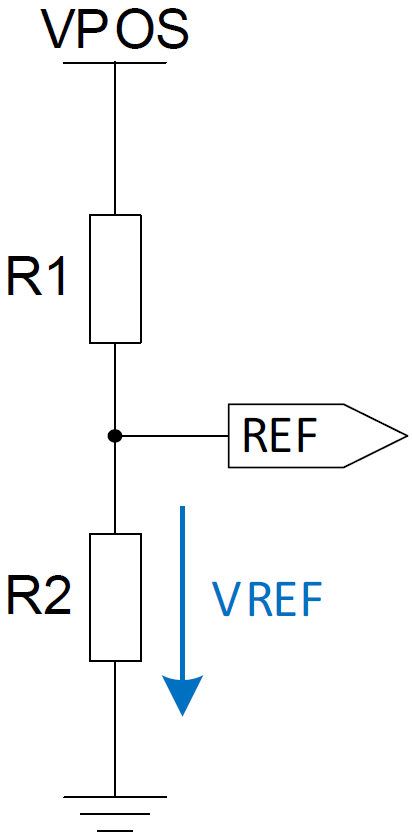
\includegraphics[width=\columnwidth]{images/spannungsteiler.png}
\end{minipage}
\hfill
\begin{minipage}[c]{0.78\columnwidth}
    \myul{\textbf{Speisespannungsabhängigkeit}}

    \begin{tabular}{ll}
        Spannungsänderung:  & $\boxed{\Delta V_{\rm ref} = \Delta V_{\rm POS} \frac{R_2}{R_1 + R_2}} $ \\
        Sensitivität:       & $\boxed{ \overunderset{V_{\rm ref}}{V_{\rm POS}}{S} = 
                                \frac{\frac{\Delta V_{\rm ref}}{\Delta V_{\rm ref}}}{\frac{\Delta V_{\rm POS}}{V_{\rm POS}}} = 1 \text{ \textrightarrow\ schlecht}}$
    \end{tabular}

    \vspace{0.2cm}
    \myul{\textbf{Temperaturabhängigkeit}} \\
    Da die Widerstände \textbf{gleiche Temperaturkoeffizienten} haben ändert sich der Strom durch $R_1$ und $R_2$, jedoch nicht das 
    Widerstandsverhältnis \textrightarrow\ $V_{\rm ref}$ bleibt \textbf{konstant} \textrightarrow\ gut

\end{minipage}

\myul{\textbf{Spannungsänderung bei Lastwechsel}}

\begin{minipage}[c]{0.2\columnwidth}
    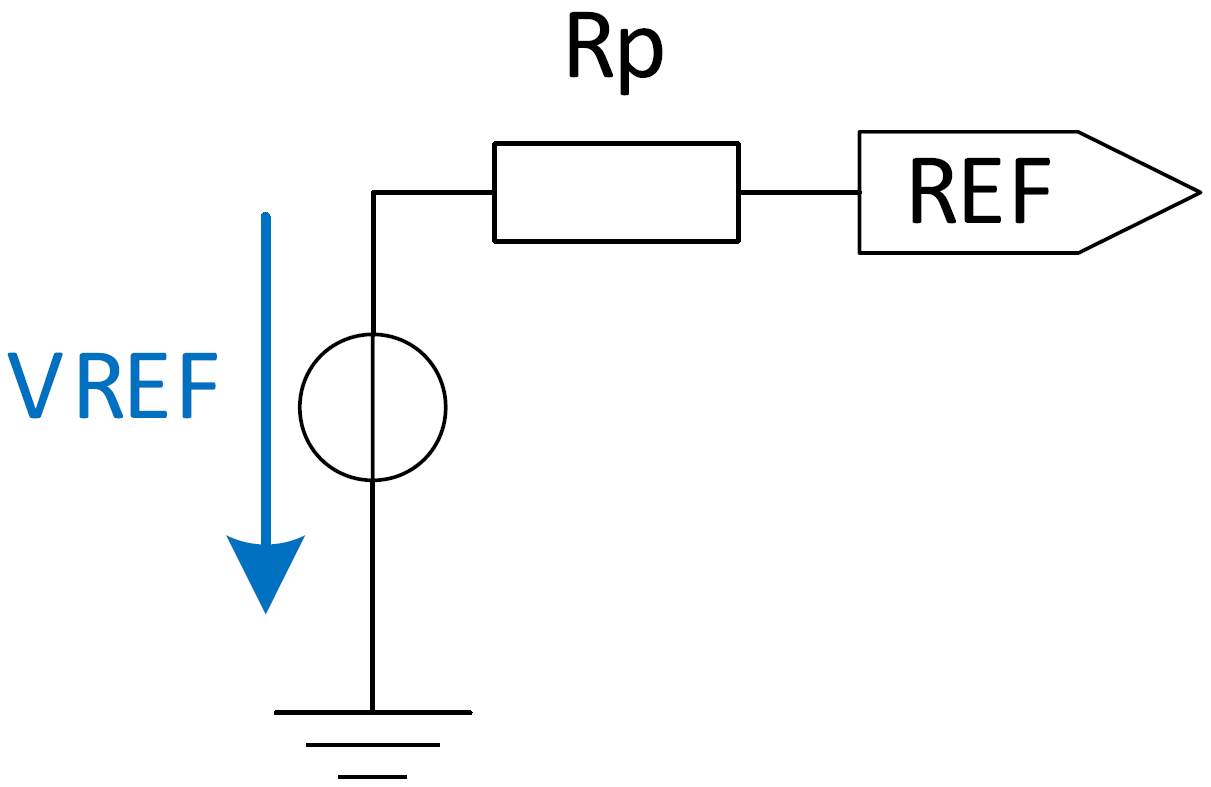
\includegraphics[width=\columnwidth]{images/thevenin.png}
\end{minipage}
\hfill
\begin{minipage}[c]{0.78\columnwidth}
    Ersatzschaltung der Referenzquelle durch Thévenin-Äquivalent mit
    $$ R_P = R_1 || R_2 \quad \text{\textrightarrow\ sehr lastabhängig, da } R_P \text{ gross} $$
\end{minipage}


\subsection{Diodenreferenz}

\begin{minipage}[c]{0.2\columnwidth}
    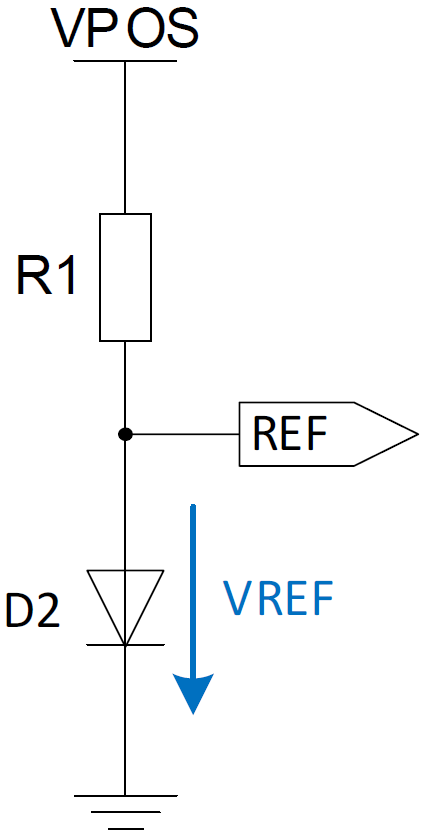
\includegraphics[width=\columnwidth]{images/diodenreferenz.png}
\end{minipage}
\hfill
\begin{minipage}[c]{0.78\columnwidth}
    $$ \boxed{ V_{\rm ref} = V_D = n \cdot V_T \cdot \ln \Big( \frac{I}{I_S} \Big) 
    \quad \text{mit } V_T =\frac{k T}{q} \approx 25 \, \milli \ampere } $$
    %$$ I = \frac{V_{\rm POS} - V_D}{R_1} \approx \frac{V_{\rm POS}}{R_1} $$ % bei Platzproblemen weglassen

    \myul{\textbf{Speisespannungsabhängigkeit}}
    
    \begin{tabular}{ll}
        Sensitivität:   & $ \boxed{ \overunderset{V_{\rm ref}}{I}{S} = \frac{1}{\ln \Big( \frac{I}{I_S} \Big)} = 0.065 \text{ \textrightarrow\ gut }} $
    \end{tabular}

    \vspace{0.2cm}
    \myul{\textbf{Temperaturabhängigkeit}} \\
    Diode hat einen \textbf{Temperaturkoeffizient von} $\boldsymbol{-2 \frac{\milli \volt}{\kelvin}}$, d.h. $V_{\rm ref}$ ändert ebenfalls
    mit ${-2 \frac{\milli \volt}{\kelvin}}$ \textrightarrow\ schlecht
\end{minipage}

\myul{\textbf{Spannungsänderung bei Lastwechsel}}

\begin{minipage}[c]{0.2\columnwidth}
    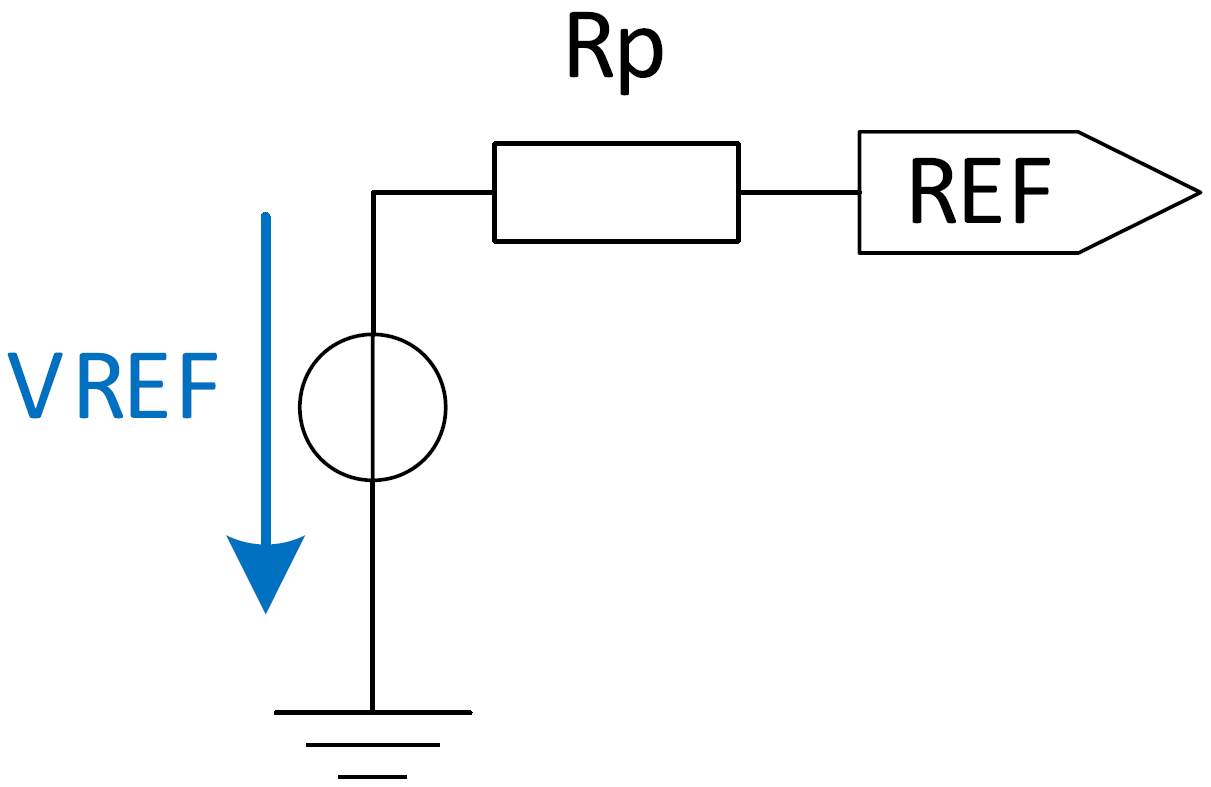
\includegraphics[width=\columnwidth]{images/thevenin.png}
\end{minipage}
\hfill
\begin{minipage}[c]{0.78\columnwidth}
    Diode durch Kleinsignal-Ersatzschaltung ersetzen und Ersatzschaltung der Referenzquelle durch Thévenin-Äquivalent mit
    $$ R_{\rm P} = R_1 || r_D \quad \text{\textrightarrow\ weniger lastabhängig, da } r_D = \frac{n \cdot V_T}{I_D} \approx 7 \, \ohm $$
\end{minipage}


\subsection{Spannungsreferenz mit mehreren Dioden}

\begin{minipage}[c]{0.25\columnwidth}
    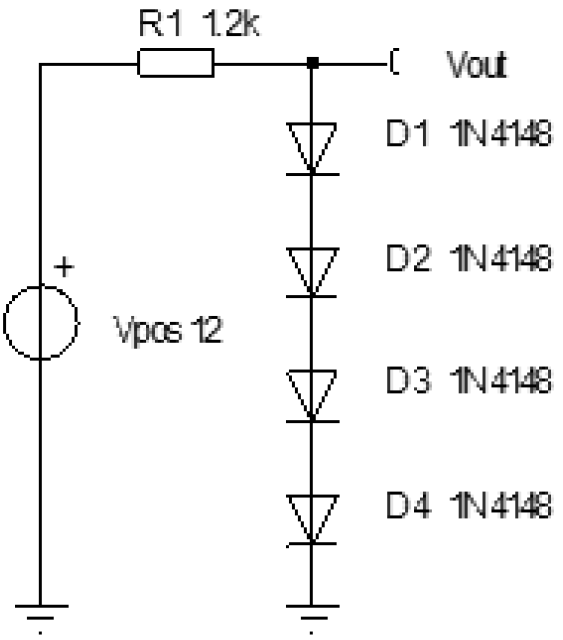
\includegraphics[width=\columnwidth]{images/spannungsreferenz_4_dioden.png}
\end{minipage}
\hfill
\begin{minipage}[c]{0.73\columnwidth}
    $m = $ Anzahl Dioden in Serie (links: $m = 4$) 

    \begin{itemize}
        \item Strom durch Dioden muss $> 0 \, \ampere$ sein, damit $V_D \approx 0.7 \, \volt$
        \item Spannung über $m$ Dioden: $ \boxed{ V_{\rm out} = m \cdot V_D }$
        \item Max. Ausgangsstrom: $ \boxed{I_{\rm out, max} =  \frac{V_{\rm pos} - V_{\rm out}}{R_1}} $
        \item \textbf{Temperaturabhängigkeit:} $TK_{\rm tot} = m \cdot -2 \frac{\milli \volt}{\kelvin}$
    \end{itemize}

\end{minipage}


\subsection{Spannungsreferenz mit Zenerdioden (Shunt-Regler)}

\textbf{Shunt-Regler:} Überflüssiger Strom wird durch ein Element abgeführt 
    \textrightarrow\ Je nach Last wird mehr oder weniger Strom in Z-Diode verheizt

\begin{minipage}[c]{0.15\columnwidth}
    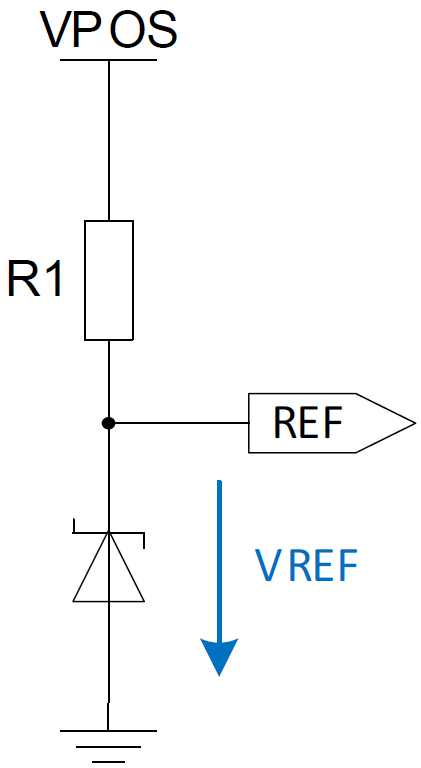
\includegraphics[width=\columnwidth]{images/spannungsreferenz_z-diode.png}
\end{minipage}
\hfill
\begin{minipage}[c]{0.78\columnwidth}
    \begin{itemize}
        \item $V_{\rm REF}$ entspricht Zener-Spannung der Z-Diode
        \item Häufigste Zener-Spannung: $5.6 \, \volt$ \textrightarrow\ TK $= 0 \frac{\milli \volt}{\kelvin}$
        \item Strom $I = \frac{V_{\rm POS} - V_{\rm REF}}{R_1}$ fliesst entweder durch Diode oder durch Last
        \item $I_{\rm out} < I_{\rm out, max} = \frac{V_{\rm POS} - V_{\rm REF}}{R_1}$
    \end{itemize}

\end{minipage}


\subsection[Bootstrap-Referenz (VD Stromquelle)]{Bootstrap-Referenz ($V_D$ Stromquelle)}

\begin{minipage}[c]{0.27\columnwidth}
    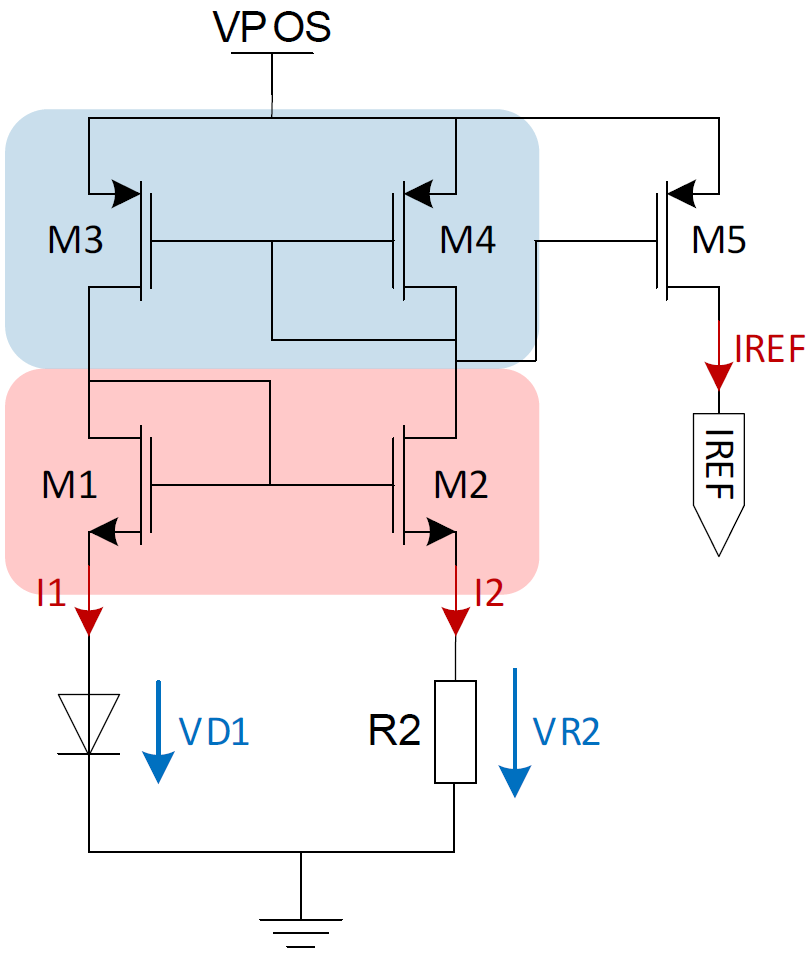
\includegraphics[width=\columnwidth]{images/bootstrap.png}
\end{minipage}
\hfill
\begin{minipage}[c]{0.71\columnwidth}
    \begin{itemize}
        \item Stromspiegel $M_3$ und $M_4$ \textrightarrow\ $I_1 = I_2$
        \item Stromspiegel $M_1$ und $M_2$ \textrightarrow\ $V_{\rm GS1} = V_{\rm GS1}$ da $I_1 = I_2$
        \item Da Temperaturkoeffizient von $V_{D1} \approx -2 \frac{\milli \volt}{\kelvin}$ nimmt $I_{\rm out}$ 
        mit steigender Temperatur ab \textrightarrow\ schlechte Referenz
        \item Schaltung hat zwei mögliche Arbeitspunkte\\
        (AP $I_1 = I_2 = 0$ ist unerwünscht!)
    \end{itemize}

    \vspace{0.2cm}
    \begin{tabular}{c c}
        $ \boxed{ V_{D1} = I_2 \cdot R_2 = V_{R2}} $ & $ \boxed{ I_{\rm REF} = I_1 = I_2 } $
    \end{tabular}
\end{minipage}


\subsection{Proportional To Absolute Temperature (PTAT)}

\begin{minipage}[c]{0.28\columnwidth}
    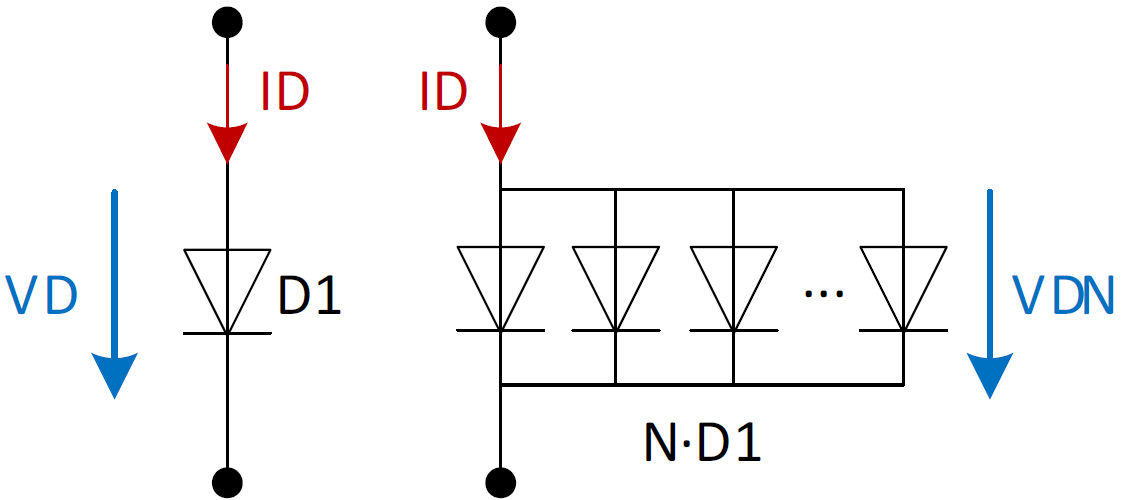
\includegraphics[width=\columnwidth]{images/ptat.png}
\end{minipage}
\hfill
\begin{minipage}[c]{0.7\columnwidth}

    \begin{tabular}{@{}c c@{}}
        $V_D = n \cdot \frac{k T}{q} \cdot \ln \Big( \frac{I_D}{I_S} \Big)$ & 
        $V_DN = n \cdot \frac{k T}{q} \cdot \ln \Big( \frac{I_D}{N \cdot I_S} \Big)$
    \end{tabular}

    $$ \boxed{ \Delta V_D = V_D - V_DN = n \cdot \frac{k T}{q} \cdot \ln(N)  = TK \cdot T }$$
    \textrightarrow $\Delta V_T$ ist proportional zur absoluten Temperatur $T$
\end{minipage}


\subsection{Bandgap-Spannungsreferenz}

\begin{minipage}[c]{0.2\columnwidth}
    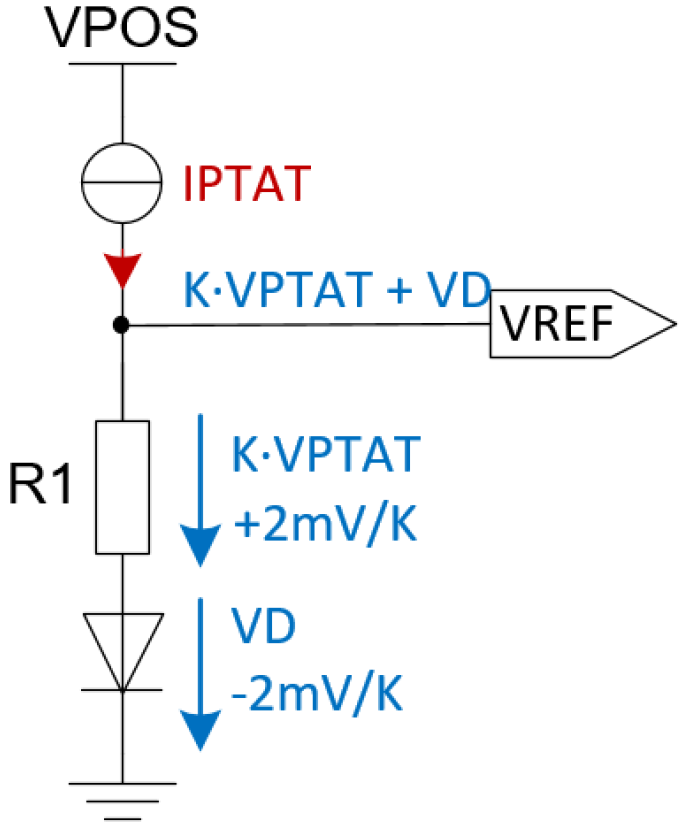
\includegraphics[width=\columnwidth]{images/bandgap_referenz.png}
\end{minipage}
\hfill
\begin{minipage}[c]{0.78\columnwidth}
    $$ \boxed{ V_{\rm REF} = K \cdot V_{\rm PTAT} + V_D } $$
    \begin{itemize}
        \item Der positive Temperaturkoeffizient von $V_{\rm PTAT}$ wird mit dem Faktor $K$ verstärkt, sodass 
            $K \cdot TK_{\rm PTAT} = +2 \frac{\milli \volt}{\kelvin}$
        \item Der nun positive Temperaturkoeffizient wird mit einer Diodenquelle mit $TK_{\rm Diode} = -2 \frac{\milli \volt}{\kelvin}$
            kompensiert
        \item Der gesamte Temperaturkoeffizient $TK_{\rm bandgap} = 0 \frac{\milli \volt}{\kelvin}$
        \item $V_{\rm REF}$ buffern, damit der Ausgang belastet werden darf
    \end{itemize}
\end{minipage}


\example{LM4041 Shunt Voltage Bandgap Reference}

\begin{minipage}[c]{0.25\columnwidth}
    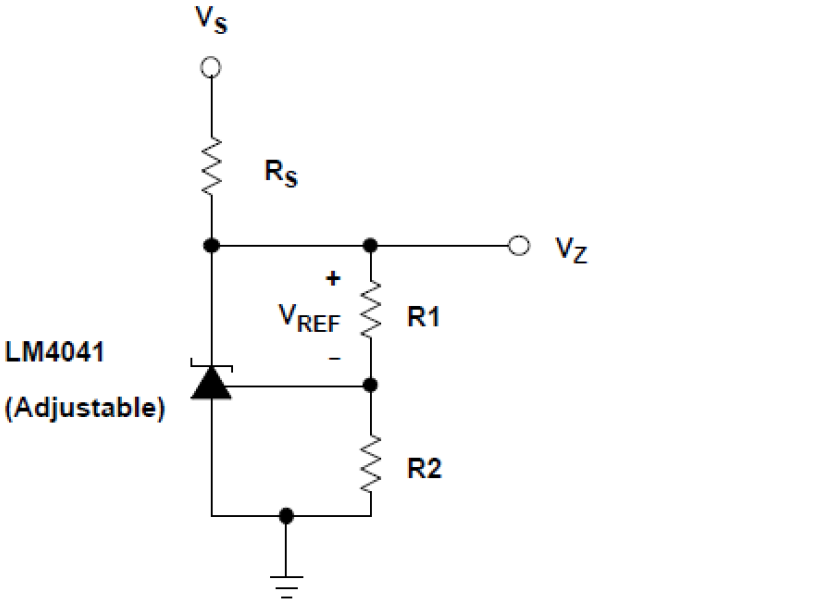
\includegraphics[width=\columnwidth]{images/beispiel_bandgap.png}
\end{minipage}
\hfill
\begin{minipage}[c]{0.72\columnwidth}
    $$ \boxed{ V_{\rm out} = V_Z = V_{\rm REF} \Big( 1 + \frac{R_2}{R_1} \Big) } $$
    \begin{itemize}
        \item Einstellbare Referenzspannung $V_Z = V_{\rm out}$
        \item Interne Referenz: $V_{\rm REF} = 1.25 \, \volt$ (Bandgap-Referenz)
    \end{itemize}
\end{minipage}


        \section{Lineare Spannungsregler}

\subsection{Spannungsstabilisierung mit Z-Diode und BJT}

\begin{minipage}[c]{0.25\columnwidth}
    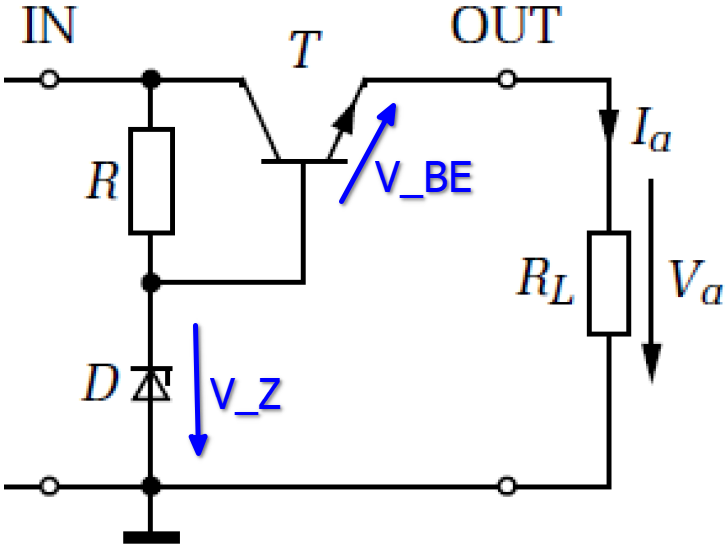
\includegraphics[width=\columnwidth]{images/spannungsstabilisierung_z-diode_bjt.png}
\end{minipage}
\hfill
\begin{minipage}[c]{0.72\columnwidth}
    $$ \boxed{ V_{out} = V_Z - V_{BE}} $$
    \begin{itemize}
        \item Ausgang kann viel Strom liefern
        \item Ausgangsspannung \textbf{sinkt} um ca. $20 \, \milli \volt$ bei \textbf{Verdoppelung} des Stroms
        \item Ausgangsspannung \textbf{sinkt} um $- 2 \frac{\milli \volt}{\kelvin}$
        \item \textbf{Keine Regelung} der Ausgangsspannung
        \item Schnell und stabil, aber nicht genau 
    \end{itemize}
\end{minipage}


\subsection{Linearer Spannungsregler}

\begin{minipage}[c]{0.3\columnwidth}
    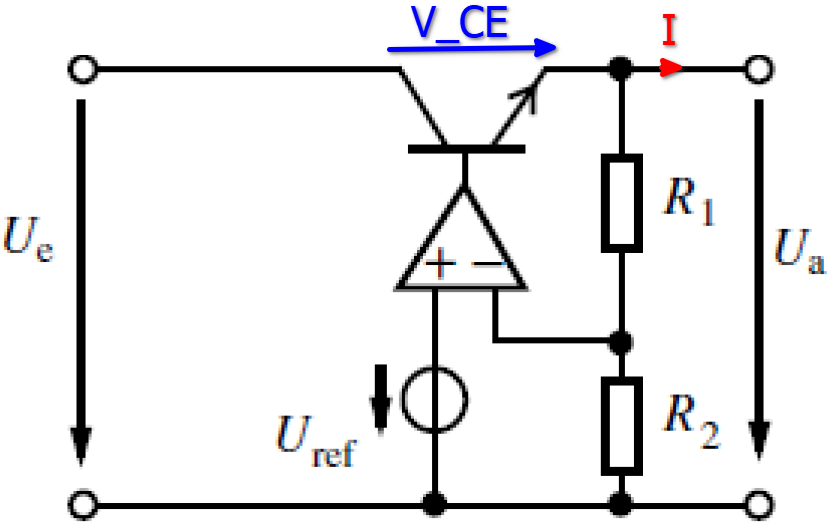
\includegraphics[width=\columnwidth]{images/linearer_spannungsregler.png}
\end{minipage}
\hfill
\begin{minipage}[c]{0.68\columnwidth}
    \begin{tabular}{c c}
        $ \boxed{ V_a = V_{ref} \Big( 1 + \frac{R_1}{R_2} \Big) } $ & $ \boxed{ P_V = V_{CE} \cdot I} $
    \end{tabular}
    \begin{itemize}
        \item OpAmp Ausgang ändert so lange, bis für die Spannungen gilt: $V_{R2} = V_{ref} \, (=1.25 \, \volt)$
        \item Minimaler Spannungsabfall $V_{CE}$ über Regler: bis $2.5 \, \volt$
        \item Regler kann sehr warm werden \textrightarrow\ Verlustleistung $P_V$
    \end{itemize}
\end{minipage}


\subsection{Low-Dropout-Regler mit pnp-Längstransistor (LDO)}

\begin{minipage}[c]{0.3\columnwidth}
    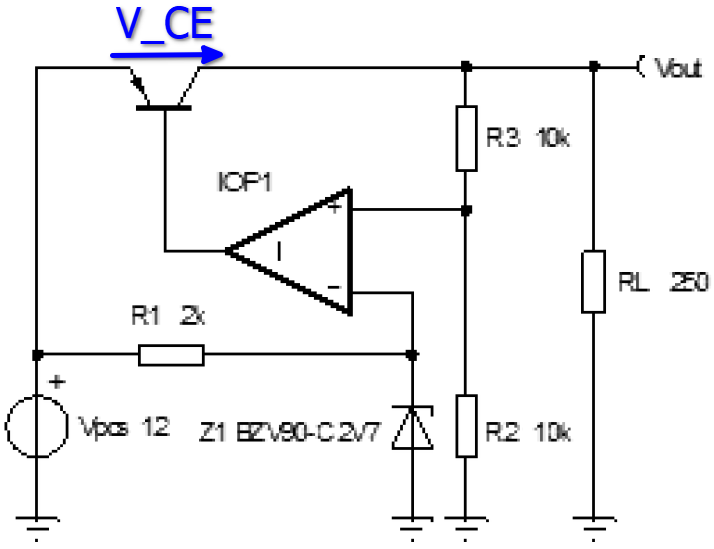
\includegraphics[width=\columnwidth]{images/ldo_pnp_transistor.png}
\end{minipage}
\hfill
\begin{minipage}[c]{0.68\columnwidth}
    \begin{itemize}
        \item Feedback auf \textbf{positiven} OpAmp-Eingang!
        \item Ansteuerung Längstransistor mit Basisspannung $< V_{out}$
        \item Kleiner minimaler Spannungsabfall $V_{CE}$ über Regler $(V_{CE,sat}$)
        \item Auch erhältlich mit PMOS-Transistor statt pnp-Transistor \textrightarrow\ Dropout-Spannung über Regler (PMOS) ist dann 
            abhängig vom Laststrom (PMOS $=$ gesteuerter Widerstand)
    \end{itemize}
\end{minipage}


\subsection{Einstellbarer Serie-Spannungsregler}

\begin{minipage}[c]{0.22\columnwidth}
    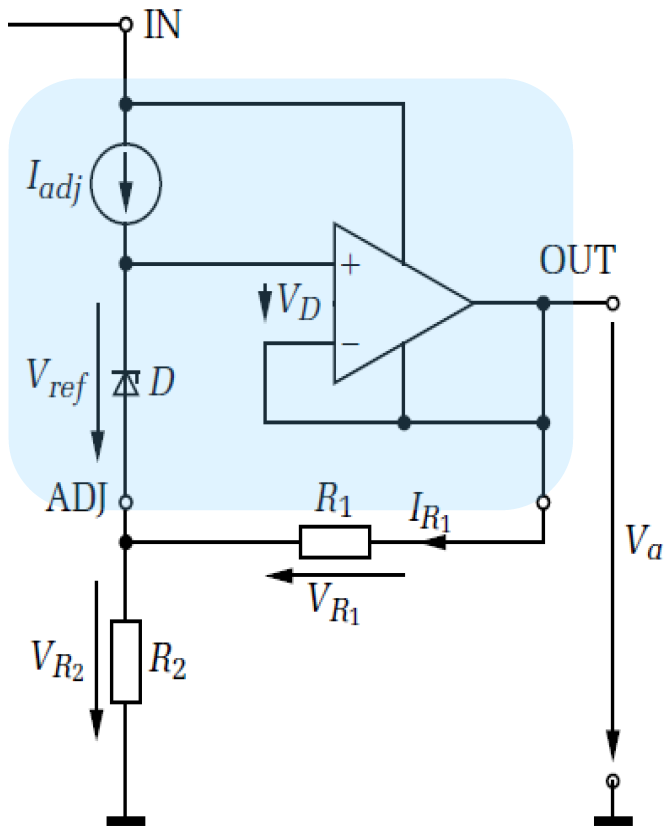
\includegraphics[width=\columnwidth]{images/einstellbarer_seriespannungsregler.png}
\end{minipage}
\hfill
\begin{minipage}[c]{0.76\columnwidth}
    % $$ \boxed{ \text{Für } I_{adj} \ll I_{R1}: \quad V_a = V_{ref} \cdot \Big( 1 + \frac{R_2}{R_1} \Big) }$$
    $$ \boxed{ V_a = V_{ref} \cdot \Big( 1 + \frac{R_2}{R_1} \Big) + I_{adj} \cdot R_2 }$$
    \begin{itemize}
        \item Widerstände $R_1$ und $R_2$ sind \textbf{extern} beschaltet!
        \item Interne Referenz: $V_{ref} = 1.25 \, \volt$ (Bandgap)
        \item OpAmp regelt, damit $V_{R1} = V_{ref}$
        \item Damit wird $V_{R2} = V_{ref} \cdot \frac{R_2}{R_1} + I_{adj} \cdot R_2$
    \end{itemize}
\end{minipage}

        \section{Spannungswandler mit Ladungspumpen}

\begin{minipage}[c]{0.72\columnwidth}
    \begin{itemize}
        \item Ladung kann \textbf{nicht springen} und nicht vernichtet werden \\
            \textrightarrow\ Ladung wird umverteilt!
        \item Ladungspumpen sind billige, effiziente Spannungswandler (Wirkungsgrad $> 99 \, \%$ möglich)
    \end{itemize}
    
\end{minipage}
\hfill
\begin{minipage}[c]{0.25\columnwidth}
    $$ \boxed{ Q = C \cdot V} $$
\end{minipage}


\subsection{Grundprinzip Switched-Capacitor-Schaltungen (SC)}

\begin{minipage}[c]{0.28\columnwidth}
    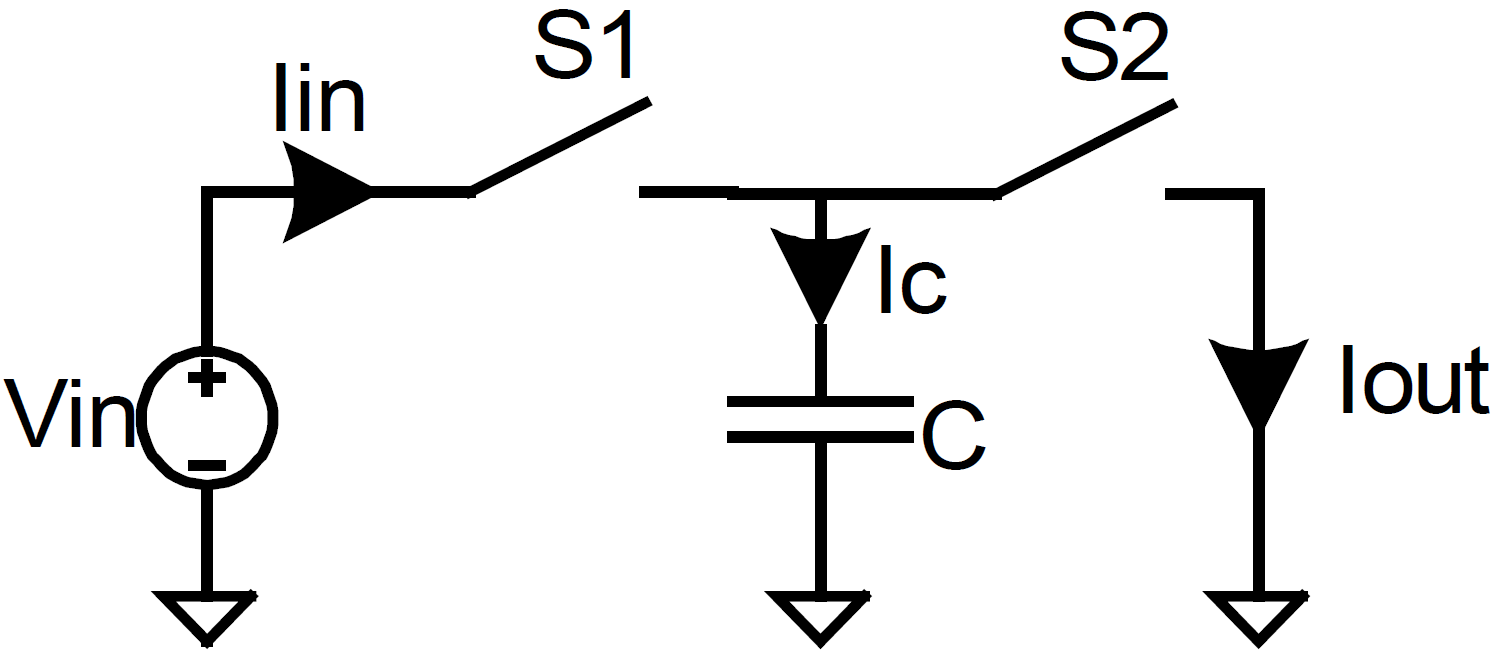
\includegraphics[width=\columnwidth]{images/grundprinzip_switched_capacitor_schaltung.png}
    \vspace{0.2cm}
    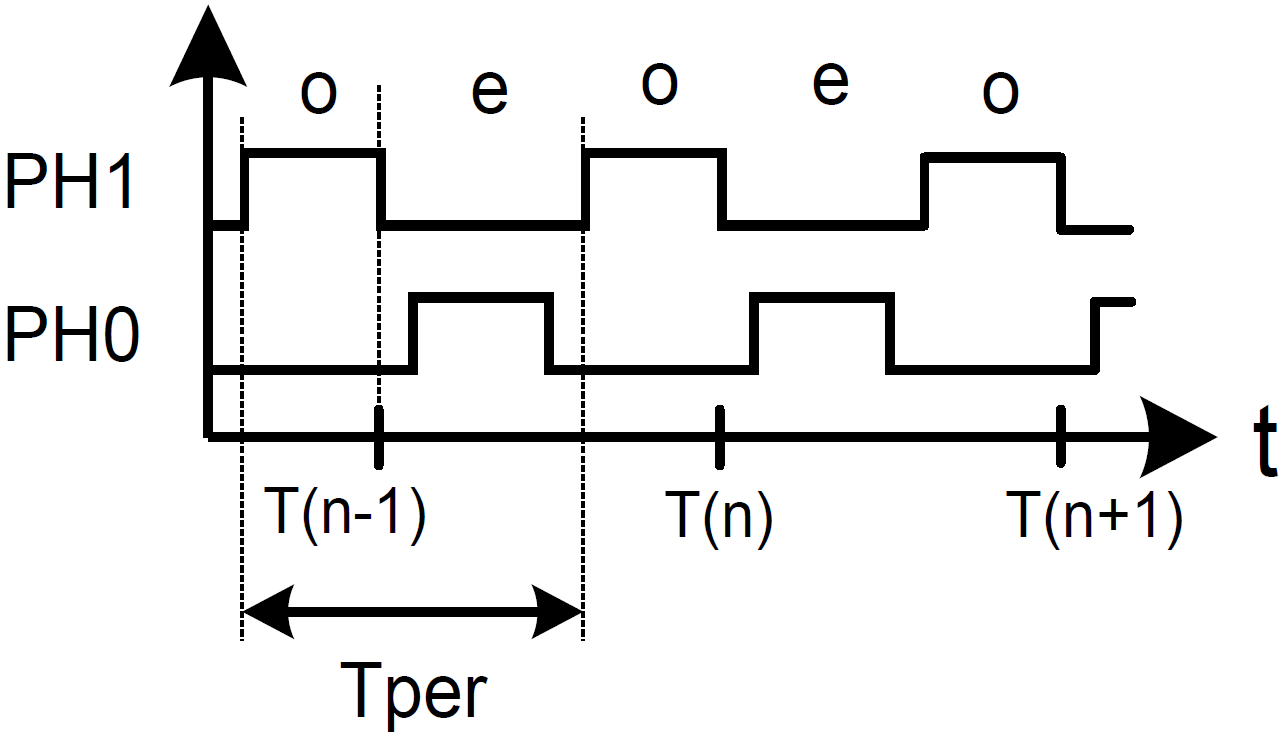
\includegraphics[width=\columnwidth]{images/grundprinzip_switched_capacitor_timing.png}
\end{minipage}
\hfill
\begin{minipage}[c]{0.7\columnwidth}
    \textbf{Hinweis:} $R_S$ entspricht dem Schalter-Widerstand \\
    Weiter gilt: $t^* = t - \frac{T}{2}$

    \begin{tabular}{ll@{}} 
        Phase PH1 (S1 geschl.)  & $I_{in} = I_C = \frac{V_{in}}{R_S} \cdot e^{\frac{t}{R_S \cdot C}} $ \\
        Phase PH2 (S2 geschl.)  & $I_C = - I_{out} = - \frac{V_{in}}{R_S} \cdot e^{\frac{t^*}{R_S \cdot C}}$ \\
        Durchschnittl. Strom    & $\overline{I_{out}} = \frac{\Delta Q}{T} =\frac{C}{T} \cdot V_{in}$ \\
    \end{tabular}

    Der 'switched capacitor' $C$ hat einen \textbf{äquivalenten Widerstand} $R_{eq} = \frac{T}{C} = \frac{1}{f \cdot C}$
\end{minipage}


\subsection{Grundprinzip Ladungspumpen}

\begin{minipage}[c]{0.5\columnwidth}
    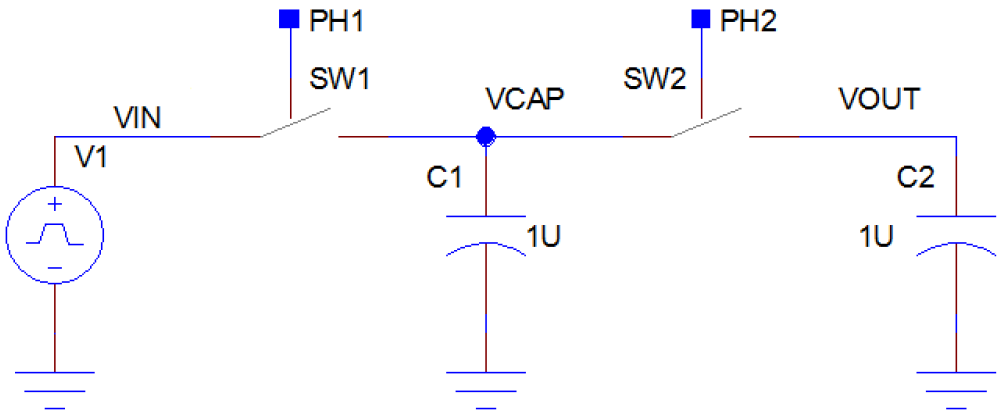
\includegraphics[width=\columnwidth]{images/grundprinzip_ladungspumpen.png} 
\end{minipage}
\hfill
\begin{minipage}[c]{0.33\columnwidth}
    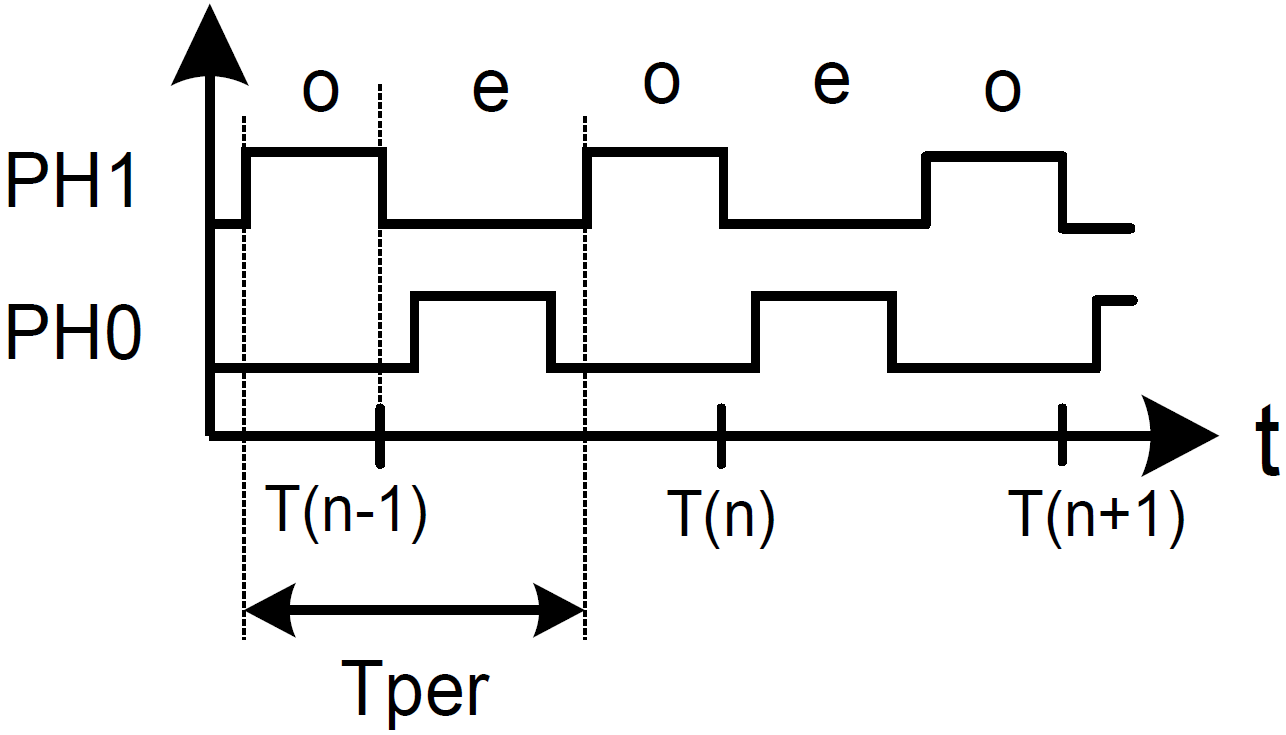
\includegraphics[width=\columnwidth]{images/grundprinzip_ladungspumpen_timing.png}
\end{minipage}

\vspace{0.2cm}
\textbf{Ausgangsspannung} $\bm{V_{out}}$ \textbf{nähert sich schrittweise exponentiell der Eingangsspannung an!} \\
Im ersten Zyklus ist $V_{out} = 0 \, \volt$

\begin{tabular}{ll@{}} 
    Phase PH1   & Kapazität $C_1$ wird auf $V_{in}$ geladen \\
                & $Q_1 = C_1 \cdot V_{in}$ und $Q_2 = C_2 \cdot V_{out}$ \\
    Phase PH2   & Ladung \textbf{verschiebt} sich von $C_1$ auf $C_2$, bis beide Kapazitäten \\
                & dieselbe Spannung aufweisen \\
                & $\cor{Q_{tot}} = Q_1 + Q_2 = C_1 \cdot V_{in} + C_2 \cdot V_{out} $ \\
                & \textrightarrow\ Neue Ausgangsspannung: $V_{out} = \frac{\cor{Q_{tot}}}{C_1 + C_2}$
\end{tabular}


\subsection{Allgemeine Funktionsweise geschaltete Kapazitäten}

\begin{minipage}[c]{0.46\columnwidth}
    \begin{center}
        \myul{Switched Capacitor $C_1$}
    \end{center}
    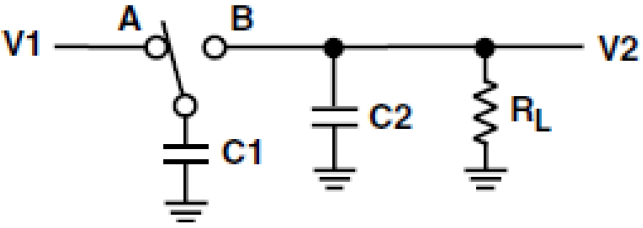
\includegraphics[width=\columnwidth]{images/sc_allgemein.png} 

    \begin{itemize}
        \item Strom fliesst in 'Paketen': \\
            $\Delta Q = C_1 \cdot \Delta V$ 
        \item Durchschnittlicher Strom proportional zu $C_1$, $\Delta V$ und Schaltfrequenz $f$
    \end{itemize}

\end{minipage}
\hfill
\begin{minipage}[c]{0.46\columnwidth}
    \begin{center}
        \myul{Ersatzschaltung mit $R_{eq}$}
    \end{center}
    \includegraphics[width=\columnwidth]{images/rc_allgemein.png}

    \begin{itemize}
        \item Durchschnittlicher Strom proportional zu $\Delta V$ und $\frac{1}{R}$
        \item Geschaltetes $C_1$ bildet äquivalenten Widerstand $R_{eq} = \frac{1}{f \cdot C_1} = \frac{T}{C}$
    \end{itemize}
\end{minipage}

\vspace{0.2cm}
Für beide Schaltungen gilt, dass der \textbf{finale Wert der Ausgangsspannung} $V_{out} = V_2$ durch den 
\textbf{Spannungsteiler} von $R_L$ und $R_{eq}$ bestimmt wird:

\begin{minipage}[c]{0.48\columnwidth}
    $$ \boxed{ V_{out} = V_{in} \cdot \frac{R_L}{R_{eq} + R_L} } $$
\end{minipage}
\hfill
\begin{minipage}[c]{0.48\columnwidth}
    $$ \boxed{ I = \frac{V_1 - V_2}{R_{eq}} } $$
\end{minipage}


\subsection{Spannungsinversion mit Switched Capacitors}

\begin{center}
    \includegraphics[width=0.75\columnwidth]{images/spannungsinverter.png}
\end{center}

\textbf{Ausgangsspannung} $\bm{V_{out}}$ \textbf{nähert sich schrittweise exponentiell $\bm{-V_{SRC}}$ an!} \\
Im ersten Zyklus ist $V_{out} = 0 \, \volt$

\begin{tabular}{ll@{}} 
    Phase PH1   & Kapazität $C_1$ wird auf $V_{SRC}$ geladen \\
                & $Q_1 = C_1 \cdot V_{SRC}$ und $Q_2 = C_2 \cdot V_{out}$ \\
    Phase PH2   & Positiver Anschluss von $C_1$ wird mit GND verbunden \\
                & \textrightarrow\ Negativer Anschluss von $C_1$ auf Potential $- V_{SRC}$ \\
                & $\cor{Q_{tot}} = Q_2 - Q_1 = C_2 \cdot V_{out} - C_1 \cdot V_{SRC}$ \\
                & \textrightarrow\ Neue Ausgangsspannung: $V_{out} = \frac{\cor{Q_{tot}}}{C_1 + C_2}$\\   % // CHECK if this is correct
\end{tabular}
\vspace{0.2cm}
Für  $C_1 = C_2$ ändert sich die Ausgangsspannung $V_{out}$ folgendermassen:
$$ V_{out} = (- \frac{1}{2}, - \frac{3}{4}, - \frac{7}{8} \cdots -1) \cdot V_{SRC} $$


\subsection{Spanungsverdoppler mit Switched Capacitors}

\begin{center}
    \includegraphics[width=0.75\columnwidth]{images/spannungsverdoppler.png}
\end{center}

\begin{itemize}
    \item PH1: $C_1$ wird auf Eingangsspannung $V_{in}$ aufgeladen
    \item PH2: Negativer Anschluss CAPN wird mit $V_{SRC}$ verbunden \textrightarrow\ Positiver Anschluss $C_1$ springt auf $2 \cdot V_{SRC} $
    \item Ladung teilt sich zwischen $C_1$ und $C_2$ auf, sodass $V_{out}$ schrittweise ansteigt 
\end{itemize}


\subsection{Dickson Charge Pump (Spannungsvervielfacher)}

\begin{minipage}[c]{0.55\columnwidth}
    \includegraphics[width=\columnwidth]{images/dickson_charge_pump.png}
\end{minipage}
\hfill
\begin{minipage}[c]{0.43\columnwidth}
    \begin{itemize}
        \item Mehrstufige Spannungsvervielfacher (hier: einstufig)
        \item Anzahl Dioden $n$ 
        \item Kaskadierung möglich
    \end{itemize}
    $$ \boxed{ V_{out} = n \cdot (V_{SRC} - V_D) } $$
\end{minipage}


\subsubsection{Mehrstufige Dickson Charge Pump}

\begin{minipage}[c]{0.5\columnwidth}
    \includegraphics[width=\columnwidth]{images/dickson_charge_pump_mehrstufig.png}
\end{minipage}
\hfill
\begin{minipage}[c]{0.48\columnwidth}
    \begin{itemize}
        \item Mehrstufige Spannungsvervielfacher (hier: $n = 5$)
    \end{itemize}

    $$ \boxed{ V_{out} = n \cdot (V_{SRC} - V_D) } $$
\end{minipage}
        \section{Schaltregler}

\textbf{SMPS} (switched-mode-power-supply) sind getaktete Systeme, deren übliche Schaltfrequenzen im Beriech von 
$20 \, \kilo \hertz$ bis zu einigen $\mega \hertz$ liegen.


% bei zu wenig Platz weglassen
\subsection{Spannungswandler mit Spulen}

\begin{outline}
    \1 \textbf{Grundprinzip}
        \2 Energie wird au einer (Spannungs-)Quelle bezogen, in verlustarmen Elementen (\textbf{Spulen}, Kondensatoren) 
            zwischengespeichert, auf die gewünschte Spannung gebracht und stabilisiert.
    \1 \textbf{Gemeinsamkeiten aller aufgeführten Spannungswandler mit Spulen}
        \2 Energie wird in Magnetfeld gespeichert $E_L = \frac{1}{2} L \cdot i_L^2$
        \2 Spannung über Spule bewirkt Änderung des Stroms \\
            $V_L = L \cdot \frac{\diff i_L}{\diff t}$ oder $I_L= \frac{1}{L} \int V_L(t) \, \diff t + I_0  = \frac{V_L}{L} \cdot t + I_0$ 
        \2 Zur Stabilisierung der Spannung werden Kondensatoren benötigt (potentieller LC-Schwingkreis!)
        \2 Für die meisten Rechnungen kann man annehmen, dass:
            \3 $V_{in}$ und $V_{out}$ \textbf{konstant} sind
            \3 Die \textbf{Schalter ideal} sind (kein Schaltwiderstand)
            \3 die\textbf{Dioden keinen Spannungsabfall} haben
\end{outline}

\textbf{Hinweis:} Zur Steigerung der Effizienz werden Dioden manchmal durch MOS-FETs ersetzt ('nur' $R_{DS,on}$ statt grosser
Spannungsabfall). Die Schalter werden in der Praxis ebenfalls mit einem FET realisiert.

\subsection{Energien in den Komponenten}

\renewcommand{\arraystretch}{1.2}
\begin{tabular}{ll}
    Energie in Spule                & $E_L = \frac{1}{2} \cdot L \cdot i_L^2$ \\
    Energie in Kondensator          & $E_C = \frac{1}{2} \cdot C \cdot V_C^2$ \\
    Energie in Last (pro Periode)   & $E_{load} = \frac{1}{2} P_{load} \cdot T_{clk} = \frac{1}{2} \cdot \frac{V_{out}^2}{R_{load}} \cdot T_{clk}$
\end{tabular}
\renewcommand{\arraystretch}{1}


\subsection{Aufwärtswandler (Boost, Step-Up Converter)}

\begin{minipage}[c]{0.4\columnwidth}
    % Aufwärtswandler (Boost, Step up)
% 
% Author:   Alex Krieg
% Date:     02.04.2024


\begin{center}
    \scalebox{0.6}{%
        \begin{circuitikz}[thick]
            % Gitternetzlinien im Hintergrund
            %\draw[xstep=1cm, ystep=1cm, line width=0.1mm, color=lightgray] (0,0) grid (6,4);

            % Einstellungen für Symbole
            \ctikzset
            {  
                inductor            =   american, 
                resistor            =   european,
                inductors/scale     =   1.0, 
                capacitors/scale    =   0.8,
                diodes/scale        =   0.6,
                line width          =   0.5,
            }
            \def\labelOffset{0.4}

            % Knoten
            \coordinate (input) at (0,2);
            \coordinate (K1) at (2,2);
            \coordinate (K2) at (4,2);
            \coordinate (output) at (5,2);
            \coordinate (G1) at (2,0);
            \coordinate (G2) at (4,0);

            % Kreuzungspunkte
            \draw (input)   node[circ]{};
            \draw (K1)      node[circ]{};
            \draw (K2)      node[circ]{};
            \draw (output)  node[circ]{};

            % Knotenbeschriftungen
            \node at ($(input)+(0,\labelOffset)$)  {$V_{IN}$};
            \node at ($(output)+(0,\labelOffset)$) {$V_{OUT}$};

            % Schaltung
            %      Start Pos    Symbol type             Name    End Pos
            \draw (input)   to [L,                      l=$L$]  (K1);               % Suple
            \draw (K1)      to [normal open switch,     l=$S$]  (G1);               % Schalter
            \draw (K1)      to [diode,                  l=$D$]  (K2);               % Diode
            \draw (K2)      to [curved capacitor,       l=$C$]  (G2);               % Kondensator
            \node at ($(G2) + (0.2,1.3)$)  {+};                                     % + Symbol am Kondensator

            \draw (K2)      to [short](output);

            \draw (G1)      node[tlground](GND){}; 
            \draw (G2)      node[tlground](GND){}; 

        \end{circuitikz}
    }
\end{center}

\end{minipage}
\hfill
\begin{minipage}[c]{0.58\columnwidth}
    \begin{center}
    \begin{tikzpicture}
        [
            scale = 0.5,
            >=latex
        ]
        \begin{axis}
            [
                width=11cm,
                height=4cm,
                xmin=0, xmax=11, ymin=0, ymax=5, axis lines=middle,
                x label style={anchor=west},
                xlabel=$t$,
                y label style={anchor=south},
                ylabel=$i(t)$,
                ticks=none
                %grid
            ]
            
            %nodes
            \node                       (m)     at (5,4)        {};
            \node                       (e)     at (10, 0)      {};
            \node[color=blue]           (s1)    at (2, 3)       {$\frac{\diff i}{\diff t} = \frac{V_L}{L}$};
            \node[color=violet]         (s2)    at (8, 3)       {$\frac{\diff i}{\diff t} = \frac{-V_L}{L}$};

            plots
            \addplot[color=blue, thick, domain=0:5]{0.8*x};
            \addplot[color=violet, thick, domain=5:10]{-0.8*x+8};
            \addplot[dashed]coordinates {(5, 0) (5, 5)};
        \end{axis}
        % \node[label={below:\tiny $t = 0$}](t0)    at (0, 0)       {};
    \end{tikzpicture}
\end{center}

\end{minipage}

\begin{tabular}{l | l}
    \textbf{\cbl{1. Phase}} Energie in Spule speichern  & \textbf{\cvt{2. Phase}} Entmagnetisierung \\
    \midrule
    \tabitem Schalter geschlossen                       & \tabitem Schalter offen \\
    \tabitem $V_L = V_{in}$ liegt an Spule an           & \tabitem Strom sinkt, wenn $V_{out} > V_{in}$ \\
    \tabitem $i_L$ muss nicht bei $I_0 = 0$ starten!    & \tabitem Eingeschwungener Zustand: $i_L = I_0$ \\
\end{tabular}

\vspace{0.2cm}
In \textbf{beiden Phasen} gelten die folgenden Formeln:

\renewcommand{\arraystretch}{1.2}
\begin{tabular}{ll}
    \cbl{Ladephase}                 & $ \Delta I_{L_{on}} = \frac{1}{L} \cdot V_{in} \cdot t_{on}$ \\
                                    & $ I_{L_{on}} = \frac{1}{L} \cdot V_{in} \cdot t_{on} + I_0 $\\ 
    \cvt{Entladephase}              & $ \Delta I_{L_{off}} = \frac{1}{L} \cdot (V_{in}- V_{out}) \cdot t_{off}$ \\ 
                                    & $I_{L_{off}} = \frac{1}{L} \cdot (V_{in}- V_{out}) \cdot t_{off} + I_0$ \\
    Gleichgewicht (eingeschwungen)  & $ \Delta I_{L_{on}} = - \Delta I_{L_{off}}$ \\ 
    Ausgangsspannung                & $V_{out} = V_{in} \cdot \Big( 1 + \frac{t_{on}}{t_{off}} \Big)$  \\
\end{tabular}
\renewcommand{\arraystretch}{1}

\vspace{0.2cm}
Die \textbf{Ausgangsspannung} $V_{out}$ ist \textbf{abhängig von der Last} 
\textrightarrow\ Bei hochohmiger Last kann die Ausgangsspannung sehr gross werden!

\subsubsection{Synchronous Boost Converter}

\begin{minipage}{0.4\columnwidth}
    \includegraphics[width=\columnwidth]{images/synchronous_boost_converter.png}
\end{minipage}
\hfill
\begin{minipage}{0.58\columnwidth}
    \begin{itemize}
        \item Diode ersetzt durch Schalter SW2
        \item Entweder SW1 \textbf{oder} SW2 geschlossen
        \item VSW somit immer leitend verbunden, entweder mit GND oder mit $V_{out}$ \\
            \textrightarrow\ In Spule fliesst immer ein Strom
    \end{itemize}
\end{minipage}

\textbf{Achtung:} Bei kleinen Lasten fliesst Strom in die Quelle zurück und die Verlustleistung in der Spule ist grösser (Drahtwiderstand)


\subsection{Aufwärtswandler: Lückender Betrieb}

\begin{minipage}{0.42\columnwidth}
    \includegraphics[width=\columnwidth]{images/boost_lueckend.png}
\end{minipage}
\hfill
\begin{minipage}{0.5\columnwidth}
    \includegraphics[width=\columnwidth]{images/boost_lueckend_timing.png}
\end{minipage}

\begin{itemize}
    \item Es existiert ein \cor{3. Zustand}, in welchem kein Strom durch Spule fliesst
    \item Aus $i_L = 0$ folgt $V_L = 0$
    \item Schalter SW offen, damit Spannung am Knoten SW $= V_{in}$ wird \textrightarrow\ Diode sperrt
    \item Control schliesst Schalter, nachdem $V_{out} < V_{out,soll}$ ist \textrightarrow\ \textbf{Regelung} von $V_{out}$
\end{itemize}


\subsubsection{Regelung der Ausgangsspannung: voltage-mode control}

\begin{minipage}{0.42\columnwidth}
    \includegraphics[width=\columnwidth]{images/regelung_ausgangsspannung_voltage.png}
\end{minipage}
\hfill
\begin{minipage}{0.56\columnwidth}
    \begin{itemize}
        \item Verstärker mit Verstäkung A0
        \item Komparator vergleicht $V_{ERROR}$ mit $V_{RAMP}$
        \item $V_{OUT} - V_{REF} \, \Uparrow$,  $V_{ERROR} \Uparrow$, Schalter muss 
            länger geschlossen bleiben \textrightarrow\ grösserer Duty Cycle \textrightarrow\ $V_{OUT} \, \Uparrow$
    \end{itemize}
\end{minipage}


\subsubsection{Regelung der Ausgangsspannung: current-mode control}

\begin{minipage}{0.42\columnwidth}
    \includegraphics[width=\columnwidth]{images/regelung_ausgangsspannung_current.png}
\end{minipage}
\hfill
\begin{minipage}{0.56\columnwidth}
    \begin{itemize}
        \item Strom wird mit Shund-Widerstand durch Spannung $V_{SENSE}$ gemessen
        \item Verstärker mit Verstäkung A0
        \item Komparator resettiert Flip-Flop \textrightarrow\ Schalter (FET) öffnet
        \item Häufiger zur Regelung verwendet als vorherige Schaltung
    \end{itemize}
\end{minipage}


\subsection{Abwärtswandler (Buck, Step-Down Converter)}

\begin{minipage}[c]{0.4\columnwidth}
    % Abwärtswandler (Buck, Step Down Converter)
% 
% Author:   Alex Krieg
% Date:     02.04.2024

\begin{center}
    \scalebox{0.6}{%
            \begin{circuitikz}[thick]
            % Gitternetzlinien im Hintergrund
            %\draw[xstep=1cm, ystep=1cm, line width=0.1mm, color=lightgray] (0,0) grid (6,4);

            % Einstellungen für Symbole
            \ctikzset
            {  
                inductor            =   american, 
                resistor            =   european,
                inductors/scale     =   1.0, 
                capacitors/scale    =   0.8,
                diodes/scale        =   0.6,
                line width          =   0.5,
            }
            \def\labelOffset{0.4}

            % Knoten
            \coordinate (input) at (0,2);
            \coordinate (K1) at (2,2);
            \coordinate (K2) at (4,2);
            \coordinate (output) at (5,2);
            \coordinate (G1) at (2,0);
            \coordinate (G2) at (4,0);

            % Kreuzungspunkte
            \draw (input)   node[circ]{};
            \draw (K1)      node[circ]{};
            \draw (K2)      node[circ]{};
            \draw (output)  node[circ]{};

            % Knotenbeschriftungen
            \node at ($(input)+(0,\labelOffset)$)  {$V_{IN}$};
            \node at ($(output)+(0,\labelOffset)$) {$V_{OUT}$};

            % Schaltung
            %      Start Pos    Symbol type             Name    End Pos
            \draw (input)   to [normal open switch,     l=$S$]  (K1);               % Schalter
            \draw (K1)      to [L,                      l=$L$]  (K2);               % Suple
            \draw (G1)      to [diode,                  l=$D$]  (K1);               % Diode
            \draw (K2)      to [curved capacitor,       l=$C$]  (G2);               % Kondensator
            \node at ($(G2) + (0.2,1.3)$)  {+};                                     % + Symbol am Kondensator

            \draw (K2)      to [short](output);

            \draw (G1)      node[tlground](GND){}; 
            \draw (G2)      node[tlground](GND){}; 
        \end{circuitikz}
    }
\end{center}
\end{minipage}
\hfill
\begin{minipage}[c]{0.58\columnwidth}
    \begin{center}
    \begin{tikzpicture}
        [
            scale = 0.5,
            >=latex
        ]
        \begin{axis}
            [
                width=11cm,
                height=4cm,
                xmin=0, xmax=11, ymin=0, ymax=5, axis lines=middle,
                x label style={anchor=west},
                xlabel=$t$,
                y label style={anchor=south},
                ylabel=$i(t)$,
                ticks=none
                %grid
            ]
            
            %nodes
            \node                       (m)     at (5,4)        {};
            \node                       (e)     at (10, 0)      {};
            \node[color=blue]           (s1)    at (2, 3)       {$\frac{\diff i}{\diff t} = \frac{V_L}{L}$};
            \node[color=violet]         (s2)    at (8, 3)       {$\frac{\diff i}{\diff t} = \frac{-V_L}{L}$};

            plots
            \addplot[color=blue, thick, domain=0:5]{0.8*x};
            \addplot[color=violet, thick, domain=5:10]{-0.8*x+8};
            \addplot[dashed]coordinates {(5, 0) (5, 5)};
        \end{axis}
        % \node[label={below:\tiny $t = 0$}](t0)    at (0, 0)       {};
    \end{tikzpicture}
\end{center}

\end{minipage}

\vspace{0.2cm}
\textbf{Vereinfachungen:} $V_{out}$ konstant, kein Spannungsabfall über Diode und Schalter \\
\textbf{Formeln gelten nur, wenn immer ein Strom in der Spule fliesst}
\vspace{0.2cm}

\renewcommand{\arraystretch}{1.2}
\begin{tabular}{ll}
    \cbl{Ladephase}                 & $ \Delta I_{L_{on}} = \frac{1}{L} \cdot (V_{in}- V_{out}) \cdot t_{on}$ \\
                                    & $ I_{L_{on}} = \frac{1}{L} \cdot (V_{in}- V_{out}) \cdot t_{on} + I_0 $\\ 
    \cvt{Entladephase}              & $ \Delta I_{L_{off}} = - \frac{1}{L} \cdot V_{out} \cdot t_{off}$ \\ 
                                    & $I_{L_{off}} = - \frac{1}{L} \cdot V_{out} \cdot t_{off} + I_0$ \\
    Gleichgewicht (eingeschwungen)  & $ \Delta I_{L_{on}} = - \Delta I_{L_{off}}$ \\ 
    Ausgangsspannung                & $V_{out} = V_{in} \cdot \frac{t_{on}}{T}$
\end{tabular}
\renewcommand{\arraystretch}{1}


\subsection{Invertierender Wandler (Buck-Boost Converter)}

\begin{minipage}[c]{0.4\columnwidth}
    % Inverting (Invertierender Wandler)
% 
% Author:   Alex Krieg
% Date:     02.04.2024


\begin{center}
    \scalebox{0.6}{%
        \begin{circuitikz}[thick]
            % Gitternetzlinien im Hintergrund
            %\draw[xstep=1cm, ystep=1cm, line width=0.1mm, color=lightgray] (0,0) grid (6,4);

            % Einstellungen für Symbole
            \ctikzset
            {  
                inductor            =   american, 
                resistor            =   european,
                inductors/scale     =   1.0, 
                capacitors/scale    =   0.8,
                diodes/scale        =   0.6,
                line width          =   0.5,
            }
            \def\labelOffset{0.4}

            % Knoten
            \coordinate (input) at (0,2);
            \coordinate (K1) at (2,2);
            \coordinate (K2) at (4,2);
            \coordinate (output) at (5,2);
            \coordinate (G1) at (2,0);
            \coordinate (G2) at (4,0);

            % Kreuzungspunkte
            \draw (input)   node[circ]{};
            \draw (K1)      node[circ]{};
            \draw (K2)      node[circ]{};
            \draw (output)  node[circ]{};

            % Knotenbeschriftungen
            \node at ($(input)+(0,\labelOffset)$)  {$V_{IN}$};
            \node at ($(output)+(0,\labelOffset)$) {$V_{OUT}$};

            % Schaltung
            %      Start Pos    Symbol type             Name    End Pos
            \draw (input)   to [normal open switch,     l=$S$]  (K1);               % Schalter
            \draw (K1)      to [L,                      l=$L$]  (G1);               % Suple
            \draw (K2)      to [diode,                  l=$D$]  (K1);               % Diode
            \draw (G2)      to [curved capacitor,       l=$C$]  (K2);               % Kondensator
            \node at ($(G2) + (0.2,0.7)$)  {+};                                     % + Symbol am Kondensator

            \draw (K2)      to [short](output);

            \draw (G1)      node[tlground](GND){}; 
            \draw (G2)      node[tlground](GND){}; 
        \end{circuitikz}
    }
\end{center}


\end{minipage}
\hfill
\begin{minipage}[c]{0.46\columnwidth}
    \includegraphics[width=\columnwidth]{images/buck_boost_timing.png}
\end{minipage}

\textbf{Der Converter kann im buck-mode oder boost-mode betrieben werden}
buck-mode: Duty Cycle $\frac{t_{on}}{T} < 0.5$ ; boost-mode: Duty Cycle $\frac{t_{on}}{T} > 0.5$ 

\begin{tabular}{ll}
    \cbl{Ladephase}                     & $ \Delta I_{L_{on}} = \frac{1}{L} \cdot V_{in} \cdot t_{on}$ \\
    \cvt{Entladephase} ($V_{out} < 0$)  & $ \Delta I_{L_{off}} = \frac{1}{L} \cdot V_{out} \cdot t_{off}$ \\ 
    Gleichgewicht (eingeschwungen)      & $ \Delta I_{L_{on}} = - \Delta I_{L_{off}}$ \\ 
    Ausgangsspannung                    & $V_{out} = - V_{in} \cdot \frac{t_{on}}{t_{off}}$  \\
\end{tabular}
\renewcommand{\arraystretch}{1}


\subsection{Flyback (Sperrwandler)}

\begin{minipage}[c]{0.4\columnwidth}
    \begin{center}
    \scalebox{0.5}{%
        \begin{circuitikz}[thick]
            %\draw[xstep=1cm, ystep=1cm, line width=0.1mm, color=lightgray] (0,0) grid (10cm,10cm);

            % Einstellungen für Symbole
            \ctikzset{
                inductor            =   american,
                inductors/scale     =   1.0,
                capacitors/scale    =   0.8,
                diodes/scale        =   0.6,
                line width          =   0.5,
            }
            \def\labelOffset{0.4}

            % Knoten
            \coordinate (input) at (0,3);
            \coordinate (P1) at (0,1);
            \coordinate (K1) at (6,3);
            \coordinate (K2) at (6,1);
            \coordinate (G) at (0,0.5);
            \coordinate (output1) at ($(K1) + (1,0)$);
            \coordinate (output2) at ($(K2) + (1,0)$);

            % Kreuzungspunkte
            \draw (input)   node[circ]{};
            \draw (K1)      node[circ]{};
            \draw (K2)      node[circ]{};
            \draw (output1)      node[circ]{};
            \draw (output2)      node[circ]{};

            % Knotenbeschriftungen
            \node at ($(input)+(0,\labelOffset)$)  {$V_{IN}$};
            \node at ($(output1)+(0,\labelOffset)$) {$V_{OUT}$};

            %Trafo%
            \draw (3,2) node[transformer, scale=0.95] (T) {}
            (T.A1) node[anchor=east] {} %A1
            (T.A2) node[anchor=east] {} %A2
            (T.B1) node[anchor=west] {} %B1
            (T.B2) node[anchor=west] {} %B2
            (T.base) node{T}
            (T.inner dot A2) node[circ]{}
            (T.inner dot B1) node[circ]{};

            %      Start Pos    Symbol type             Name        End Pos
            \draw (G)         node[tlground                    ]  {};             % GND
            \draw (0,1)         to [normal open switch,     l=$S$]  (T.A2) {};      % Switch
            \draw (T.B1)        to [diode,                  l=$D$]  (K1);          % Diode
            \draw (K1)          to [curved capacitor,       l=$C$]  (K2);           % Kondensator
            \node at ($(K2) + (0.2,1.3)$)  {+};                                     % + Symbol am Kondensator

            % Verbindungen
            \draw (input) [short] (T.A1);
            \draw (G) |- (0.1,1);
            \draw (input) -- (T.A1);
            \draw (T.B2) -- (output2);
            \draw (K1) -- (output1);

        \end{circuitikz}
    }
\end{center}


\end{minipage}
\hfill
\begin{minipage}[c]{0.58\columnwidth}
    \begin{itemize}
        \item Ermöglicht \textbf{galvanische Trennung} zwischen Ein- und Ausgang
        \item Transformator mit grosser Induktivität nötig zur Energiespeicherung (mit Luftspalt)
    \end{itemize}
\end{minipage}


\begin{outline}
    \1 Phase 1 (Schalter geschlossen)
        \2 Linear steigender Strom auf Primärseite; Energie wird im Magnetfeld gespeichert
    \1 Phase 2 (Schalter offen)
        \2 Linear sinkender Strom auf Sekundärseite; Magnetfeld baut sich über Sekundärspule ab
    \1 Phase 3 (LC-Schwingkreis)
        \2C parallel zu Schalter auf Primärseite wird wirksam 
\end{outline}


\subsection{Power Fail Control (PFC)}

\begin{minipage}[c]{0.42\columnwidth}
    \includegraphics[width=\columnwidth]{images/pfc_schaltung.png}
\end{minipage}
\hfill
\begin{minipage}[c]{0.42\columnwidth}
    \includegraphics[width=\columnwidth]{images/pfc.png}
\end{minipage}

\begin{minipage}[c]{0.48\columnwidth}
    \begin{center}
        \myul{Ohne PFC}
    \end{center}
    \begin{itemize}
        \item Strom fliesst nur wenn $V_{in} > V_C$\\
            (nur bei Spannungsmaximum) \\
            \textrightarrow\ erzeugt Oberwellen (Blindleistung)
    \end{itemize}
\end{minipage}
\hfill
\begin{minipage}[c]{0.48\columnwidth}
    \begin{center}
        \myul{Mit PFC}
    \end{center}
    \begin{itemize}
        \item Strom soll \textbf{möglichst sinusförmig} fliessen, nicht nur beim Spannungsmaximum
        \item Lösung: 1. Stufe mit Boost Converter
    \end{itemize}
\end{minipage}


\subsection{Aufbau Modernes Netzteil}

\includegraphics[width=\columnwidth]{images/modernes_netzteil.png}

\begin{itemize}
    \item 1. Stufe: Gleichrichtung und Boost Converter mit PFC
    \item 2. Stufe: Reduktion auf Systemspannung (Bus voltage) mit Flyback-Converter
    \item 3. Stufe: Buck Converter (ev. mehrere)
\end{itemize}


\subsection{Fazit Spannungswandler SMPS}

\begin{itemize}
    \item Geschaltete Spannungsregler generrieren weniger Verlustleistung als Linearregler
    \item Ausgangsspannung geschalteter Spannungsregler hat \textbf{Rippel} der Schaltfrequenz \\
        \textrightarrow\ Muss ev. mit Linearrregler zusätzlich stabilisiert werden
\end{itemize}
        \section{Passive Filter}

\begin{tabular}{ll@{}}
    $f_{3 \, \deci \bel}$   & Cut-Off-Frequency, Corner-Frequency \\
                            & Dämpfung von $3 \, \deci \bel$ (d.h. Amplitude wird mit $\frac{1}{\sqrt{2}}$ 'verstärkt'), Phase: $- 45 \degree$ \\
    $f_S$                   & Sampling-Frequenz (ADC, digitale Filter) \\
                            & \textrightarrow\ Alle Frequenzen über $\frac{f_S}{2}$ müssen unterdrückt werden \\
    UTF                     & Übertragungsfunktion $G(s)$
\end{tabular}


\subsection{Tiefpassfilter 1. Ordnung}

\begin{minipage}[c]{0.3\columnwidth}
    \includegraphics[width=\columnwidth]{images/tiefpass_ordnung_1.png}
\end{minipage}
\hfill
\begin{minipage}[c]{0.45\columnwidth}
    % $$ \text{UTF: } G(s) = \frac{V_{\rm out}}{V_{\rm in}} = \frac{\frac{1}{s \cdot C}}{R + \frac{1}{s \cdot C}} = \frac{1}{1 + s \cdot \underbrace{R \cdot C}_T} $$
    $$ \boxed{ G(s) = \frac{V_{\rm out}}{V_{\rm in}} = \frac{1}{1 + s \cdot \underbrace{R \cdot C}_T} } $$
\end{minipage}
\hfill
\begin{minipage}[c]{0.23\columnwidth}
    $$ \boxed{ f_{3 \, \deci \bel} = \frac{1}{2 \pi \underbrace{R C}_T} } $$
\end{minipage}

\textbf{Hinweis:} Die Zeitkonstante $T$ entspricht immer dem Parameter vor dem $s$. 
Beim Tiefpass 1. Ordnung entspricht dies $T = R \cdot C$


\subsection{Bodeplot Tiefpassfilter 1. und 2. Ordnung}

\begin{minipage}[t]{0.48\columnwidth}
    \begin{center}
        \myul{1. Ordnung}
    \end{center}
    \begin{itemize}
        \item Abfall von $- 20\, \deci \bel$ / Dekade
        \item Phasenschiebung von maximal $- 90 \degree$ (bei $f_g = -45 \degree$)
    \end{itemize}
\end{minipage}
\hfill
\begin{minipage}[t]{0.48\columnwidth}
    \begin{center}
        \myul{2. Ordnung}
    \end{center}
    \begin{itemize}
        \item Abfall von $- 40\, \deci \bel$ / Dekade
        \item Phasenschiebung von maximal $- 180 \degree$ (bei $f_g = -90 \degree$)
    \end{itemize}
\end{minipage}


\subsection{Filter 2. Ordnung}

\subsubsection{Kaskadierung von zwei gleichen Filtern}

\begin{minipage}[c]{0.48\columnwidth}
    $$ G_{11}(s) = \frac{1}{1 + s \cdot \underbrace{R \cdot C}_{T_2}} \cdot \frac{1}{1 + s \cdot \underbrace{R \cdot C}_{T_2}} $$
\end{minipage}
\hfill
\begin{minipage}[c]{0.48\columnwidth}
    $$ T_2 = \frac{\sqrt{\sqrt{2} - 1}}{2 \pi f_{3 \, \deci \bel} } \approx 0.64 \cdot T_1  $$
\end{minipage}

Daraus folgt, dass bei 2 identischen Stufen die Grenzfrequenz $f_{3 \, \deci \bel}$ der einzelnen Stufen $\frac{1}{0.64} = 1.56$ mal 
\textbf{höher} gewählt werden muss als bei einem Filter 1. Ordnung.


\subsubsection{Filter 2. Ordnung mit komplexen Polen}

\begin{minipage}[c]{0.6\columnwidth}
    $$ G(s) = \frac{A_0 \cdot p_1 \cdot p_2}{(p_1 + s) \cdot (p_2 + s)} = \frac{A_0 \cdot \omega_0^2}{s^2 + \frac{\omega_0}{Q} s + \omega_0^2} $$
$$ p_{1,2} = \frac{\omega_0}{2 Q} (1 \pm \sqrt{1 - 4 Q^2}) $$
\end{minipage}
\hfill
\begin{minipage}[c]{0.38\columnwidth}
    \begin{tabular}{ll}
        $p_i$       & Polstellen \\
                    & komplex für $Q > \frac{1}{2}$ \\
        $Q$         & Polgüte / Filtergüte \\
        $\omega_0$  & Polfrequenz
    \end{tabular}
\end{minipage}


% bei Platzmangel weglassen
\subsection{Filter höherer Ordnung}

\begin{itemize}
    \item Systeme höherer Ordnung können in kaskadierte Teilsysteme 1. \& 2. Ordnung aufgeteilt werden
    \item Höhere Ordnung und komplexe Pole ermöglichen steileren Übergang zwischen Durchlass- und Sperrbereich
\end{itemize}

Folgende Filter erzielen durch unterschiedliche Polverteilungen untersch. Verhalten:

\begin{itemize}
    \item \textbf{Butterworth:} Konstant im Durchlassbereich der UTF
    \item \textbf{Bessel:} Beste Rechteckübertragung, kein Überschwingen
    \item \textbf{Tschebyscheff:} Steilster Abfall im Sperrbereich der UTF
\end{itemize}


\subsection{Zeitverhalten: Schrittantwort}

\begin{enumerate}
    \item Frenqenzbereich: \textbf{Multiplikation} der UTF mit $\frac{1}{s}$
    \item Rücktransformation in den Zeitbereich, um $t_{\rm step}(t)$ zu erhalten
\end{enumerate}


\subsubsection{Tiefpass 1. Ordnung}

\begin{minipage}[c]{0.48\columnwidth}
    \includegraphics[width=\columnwidth]{images/schrittantwort_tp_ordnung_1.png}
\end{minipage}
\hfill
\begin{minipage}[c]{0.48\columnwidth}
    $$  t_{\rm step,1}(t) = 1 - e^{- \frac{t}{T_1}} $$
\end{minipage}


\subsubsection{Tiefpass 2. Ordnung}

\begin{minipage}[c]{0.43\columnwidth}
    \includegraphics[width=\columnwidth]{images/schrittantworten_vergleich.png}
\end{minipage}
\hfill
\begin{minipage}[c]{0.55\columnwidth}
    $$ t_{\rm step2a}(t) = 1 - e^{- \frac{t}{T_1}}\cdot \left\lgroup 1 + \frac{t}{T_1} \right\rgroup $$
    $$ t_{\rm step2b}(t) = 1 - \left\lgroup \frac{T_1 \cdot e^{- \frac{t}{T_1}} - T_2 \cdot e^{- \frac{t}{T_2}}}{T_1 - T_2} \right\rgroup $$
\end{minipage}


\subsection{Schrittantworten verschiedener Polgüten}

\begin{minipage}[c]{0.48\columnwidth}
    \includegraphics[width=\columnwidth]{images/schrittantwort_verschiedene_polgueten.png}
\end{minipage}
\hfill
\begin{minipage}[c]{0.48\columnwidth}
    Komplexe Pole ($Q > 0$) führt zu Überschwingern. \\
    Bei einer Polgüte von $Q = \frac{1}{\sqrt{2}} \approx 0.7$ (\cgn{grüne Kurve}) schwingt das System am schnellsten ein!
\end{minipage}


\subsection{Filter 2. Ordnung (passiv und aktiv)}

% Allgmeingültig, egal ob aktive oder passive Filter
\begin{minipage}[c]{0.48\columnwidth}
    \begin{center}
        \myul{\textbf{Tiefpass}}
    \end{center}
    $$ \boxed{ G(s) = \frac{V_{\rm out}}{V_{\rm in}} = \frac{A_0}{\frac{1}{\omega_0^2} s^2 + \frac{1}{\omega_0 \cdot Q} s + 1 } } $$
\end{minipage}
\hfill
\begin{minipage}[c]{0.48\columnwidth}
    \begin{center}
        \myul{\textbf{Bandpass}}
    \end{center}
    $$ \boxed{ G(s) = \frac{V_{\rm out}}{V_{\rm in}} = \frac{A \cdot \frac{\omega_0}{Q} \cdot s}{s^2 +  \frac{1}{ \omega_0 \cdot Q} s + 1 } } $$
\end{minipage}

\vspace{0.2cm}

\begin{minipage}[t]{0.48\columnwidth}
    \begin{center}
        \myul{\textbf{Hochpass}}
    \end{center}
    $$ \boxed{ G(s) = \frac{V_{\rm out}}{V_{\rm in}} = \frac{A_0 \cdot \frac{1}{\omega_0^2} \cdot s^2}{\frac{1}{\omega_0^2} s^2 + \frac{\omega_0}{Q} s + \omega_0^2 } } $$
\end{minipage}
\hfill
\begin{minipage}[t]{0.48\columnwidth}
    \begin{center}
        \myul{\textbf{Aufbau Nenner}}
    \end{center}
    \begin{outline}
        \1 Alle Terme positiv
        \1 $s^2$-Term definiert Grenzfrequenz
        \1 Im $s$-Term ist Dämpfung enthalten
            \2 $s$-Term gross \textrightarrow\ grosse Dämpfung
            \2 $s$-Term $= 0$ \textrightarrow\ Oszillator!
    \end{outline}
\end{minipage}

\vspace{0.2cm}

Passive RC-Filter können maximal Güte $0.5$ haben (entkoppelte reelle Pole). Filter höherer Güte benötigen entweder
Spulen oder \textbf{Verstärker}. \\
\textbf{\textrightarrow\ Die Formeln gelten aber für passive und aktive Filter!}



\example{UTF Tiefpass 2. Ordnung}

\begin{minipage}[c]{0.4\columnwidth}
    \includegraphics[width=\columnwidth]{images/tiefpass_ordnung_2.png}
\end{minipage}
\hfill
\begin{minipage}[c]{0.58\columnwidth}
    $$ A_0 = 1 \qquad \omega_0 = \frac{1}{\sqrt{C_1 C_2 R_1 R_2}} $$
    $$ Q = \frac{\sqrt{C_1 C_2 R_1 R_2}}{C_1 R_1 + C_2 R_1 + C_2 R_2} $$
\end{minipage}
$$ G(s) = \frac{V_{\rm out}}{V_{\rm in}} = \frac{1}{1 + (C_1 R_1 + C_2 R_1 + C_2 R_2) \cdot s + C_1 C_2 R_1 R_2 \cdot s^2 } $$
        \section{Aktive Filter} 

\subsection{Sallen-Key-Filter (Einfachmitkopplung)}

\begin{minipage}[c]{0.4\columnwidth}
    \includegraphics[width=\columnwidth]{images/sallen_key.png}
\end{minipage}
\hfill
\begin{minipage}[c]{0.58\columnwidth}
    $$ \text{OpAmp:} \quad  V_{\rm out} = G_0 \cdot V_3 = \Big(1 + \frac{R_A}{R_B} \Big) \cdot V_3 $$
    $$ \omega_0 = \frac{1}{\sqrt{C_1 C_2 R_1 R_2}} $$
    $$ Q = \frac{\sqrt{C_1 C_2 R_1 R_2}}{ C_2 (R_1 + R_2) + C_1 R_1 \cdot (1 - G_0)} $$
\end{minipage}

$$ \boxed{ G(s) = \frac{G_0}{ C_1 C_2 R_1 R_2 \cdot s^2 + [ C_2 (R_1 + R_2) + C_1 R_1 (1 - G_0) ] \cdot s + 1} } $$

\textbf{Stromgleichungen:}
\begin{align*}
    \text{V2:} \quad 0 &= (V_2 - V_{\rm in}) \frac{1}{R_1} + (V_2 - V_3) \frac{1}{R_2} + (V_2 - V_{\rm out}) \cdot s \cdot C_1  \\
    \text{V3:} \quad 0 &= (V_3 - V_2) \frac{1}{R_2} + V_3  \cdot s \cdot C_2 
\end{align*}


\subsubsection{Sallen-Key-Filter bei hohen Frequenzen}

\begin{minipage}[c]{0.4\columnwidth}  
    \includegraphics[width=\columnwidth]{images/sallen_key_hohe_frequenzen.png}
\end{minipage}
\hfill
\begin{minipage}[c]{0.58\columnwidth}
    $$ \boxed{ \frac{V_{\rm out}}{V_{\rm in}} \approx \frac{r_{\rm OL}}{R_1 + r_{\rm OL}} }$$
    $r_{\rm OL}$ ist der OpAmp open-loop Ausgangswiderstand (bei hohen Frequenzen $\approx 100 \, \ohm$)
\end{minipage}

\begin{itemize}
    \item Dämpfung ist limitiert auf obigen Spannungsteiler
        \textrightarrow\ Sallen-Key-Filter sind nicht geeignet für Systeme mit hohen Frequenzanteilen z.B. PWM-DAC
\end{itemize}


\subsection{Multiple-Feedback-Struktur}

\begin{minipage}[c]{0.4\columnwidth}
    \includegraphics[width=\columnwidth]{images/aktive_filter_multiple_feedback.png}
\end{minipage}
\hfill
\begin{minipage}[c]{0.58\columnwidth}
    $$ \text{OpAmp:} \quad  G_0 = -\frac{R_2}{R_1} $$
    $$ Q = \frac{\sqrt{C_1 C_2 R_1 R_2}}{ C_2 \Big( R_2 + R_3 + R_3 \frac{R_2}{R_1} \Big)} $$
\end{minipage}

$$ \boxed{ G(s) = \frac{G_0}{1 + C_2 \Big( R_2 + R_2 + R_3 \frac{R_2}{R_1} \Big) \cdot s + C_1 C_2 R_2 R_3 \cdot s^2 }}$$

\textbf{Stromgleichungen:}
\begin{align*}
    \text{V2:} \quad 0 &= (V_2 - V_{\rm in}) \frac{1}{R_1} + (V_2 - V_{\rm out}) \frac{1}{R_2} + (V_2 - V_3) \frac{1}{R_3} + V_2 \cdot s \cdot C_1  \\
    \text{V3:} \quad 0 &= (V_3 - V_2) \frac{1}{R_3} + (V_3 - V_{\rm out})  \cdot s \cdot C_2 
\end{align*}


\subsection{Sallen-Key vs. Multiple-Feedback Struktur}

\begin{minipage}[t]{0.48\columnwidth}
    \begin{center}
        \myul{\textbf{Sallen-Key}}
    \end{center}
    \begin{outline}
        \1 Nicht-invertierend
        \1 $Q$ sensitiver auf Toleranzen
        \1 Vorwärtspfad für hohe Frequenzen
        \1 Noise-Gain: $A$
        \1 Eher für 
            \2 Hochpass
            \2 kleine Verstärkungen
    \end{outline}
\end{minipage}
\hfill
\begin{minipage}[t]{0.48\columnwidth}
    \begin{center}
        \myul{\textbf{Multiple-Feedback}}
    \end{center}
    \begin{outline}
        \1 Invertierend
        \1 $f_g$ sensitiver auf Toleranzen 
        \1[] 
        \1 Noise-Gain: $A+1$
        \1 Eher für 
            \2 Tiefpass, Bandpass
            \2 grössere Verstärkungen
    \end{outline}
\end{minipage}


\subsection{Vorgehen: UTF aus OPV-Filterschaltung ermitteln}
\begin{itemize}
    \item Stromgleichungen (Knotengleichungen) aufstellen
    \item Gleichungen ineinander einsetzen
    \item Umformen nach $G(s) = \frac{V_{\rm out}}{V_{\rm in}}$
\end{itemize}


\subsection{Zustandsvariablen-Filter (Biquad-Filter)}
\label{zustandsvariablenfilter}

\begin{minipage}[c]{0.6\columnwidth}
    \includegraphics[width=\columnwidth]{images/zustandsvariablenfilter.png}
\end{minipage}
\hfill
\begin{minipage}[c]{0.38\columnwidth}
    \raggedright%
    Mit dieser Topologie sind alle drei \textbf{Parameter} $f_0$, $Q$ und $A_0$ \textbf{frei wählbar!} \\
    An $V_{\rm out}$ herrscht \textbf{Tiefpass-Verhalten.}
\end{minipage}

$$ \boxed{ G(s) = \frac{- \frac{R_{\rm fb}}{R_{\rm in}}}{s^2 \cdot C_{i1} C_{i2} R_{\rm fb} R_{i2} \frac{R_1}{R_2} + s \cdot C_{\rm fb} R_{\rm fb} + 1} } $$

$$ f_0 = \frac{1}{2 \pi \sqrt{C_{i1} C_{i2} R_{\rm fb} R_{i2} \frac{R_1}{R_2}}} \qquad Q = \frac{1}{C_{\rm fb}} \sqrt{C_{i1} C_{i2} \frac{R_1}{R_2 R_{\rm fb}} } 
\qquad A_0 = - \frac{R_{\rm fb}}{R_{\rm in}} $$


\subsubsection{Allgemein: Filter mit mehreren OpAmps}

Mit der Filter-Struktur aus Abschnitt~\ref{zustandsvariablenfilter} können auch Bandpass- und Hochpass-Filter gebildet werden:
\begin{itemize}
    \item \textbf{Tiefpass:} Abgriff beim 3. OpAmp ($V_{\rm out}$ gemäss Abschnitt ~\ref{zustandsvariablenfilter})
    \item \textbf{Bandpass:} Abgriff beim 2. OpAmp (an Knoten V2)
    \item \textbf{Hochpass:} Abgriff beim 2. OpAmp, Einspeisung am neg. Eingang des 2. OpAmps 
\end{itemize}


        
\section{Analyse von Filterschaltungen mit SFDs}

Aktive Filterschaltungen (mit OpAmps) können mittels Signalflussdiagrammen (SFDs) analysiert werden. Dazu wird die gesamte Schaltung
in einzelne Komponenten aufgeteilt. Diese Komponenten werden dann mit Impedanz- bzw. Admittanzfunktionen abgebildet.
Um die Übertragungsfunktion (UTF) der gesamten Schaltung zu erhalten, muss die \textbf{Regel von Mason} angewendet werden.

\subsection{Eingangsadmittanzen / (Eingangsimpedanzen)}

\textbf{Hinweis:} Es wird normalerweise mit Eingangs\textbf{admittanzen} gearbeitet!

\begin{ctabular}{lll}
    \textbf{Komponente} & \textbf{Admittanz} $\bm{Y}$       & (\textbf{Impedanz} $\bm{Z}$) \\
    \midrule
    Widerstand $R$      & $Y_{\rm res} = \frac{1}{R}$           & ($Z_{\rm res} = R$  )\\
    Kapazität $C$       & $Y_{\rm cap} = s \cdot C$             & ($Z_{\rm cap} = \frac{1}{s \cdot C}$)\\
    Induktivität $L$    & $Y_{\rm ind} = \frac{1}{s \cdot L}$   & ($Z_{\rm ind} = s \cdot L$)
\end{ctabular}


\subsection{OpAmp Impedanzfunktionen}

\textbf{Hinweis:} Es geht um \textbf{negatives Feedback} bzw. \textbf{Gegenkopplung}

\begin{ctabular}{ll}
    \textbf{Schaltung (Feedback)}       & \textbf{Impedanz} $\bm{Z}$ \\
    \midrule
    Widerstand $R_f$ im Feedback        & $Z_{\rm op} = - R_f$ \\
    Kapazität $C_f$ im Feedback         & $Z_{\rm op} = - \frac{1}{s \cdot C_f}$ \\
    $R_f C_f$ (parallel) im Feedback    & $Z_{\rm op} = - \frac{R_f}{1 + s \cdot C_f \cdot R_f}$
\end{ctabular}


\example{Summierender Verstärker}

\begin{minipage}[c]{0.4\columnwidth}
    \includegraphics[width=\columnwidth]{images/summierender_verstaerker.png}
\end{minipage}
\hfill
\begin{minipage}[c]{0.58\columnwidth}
    \begin{center}
        \includegraphics[width=0.8\columnwidth]{images/summierender_verstaerker_sfd.png}
    \end{center}
    $$ V_{\rm out} = Z_{\rm op} \cdot (Y_0 \cdot V_{\rm in0} + Y_1 \cdot V_{\rm in1}) $$
\end{minipage}

$$ Y_0 = \frac{1}{R_0} \qquad Y_1 = \frac{1}{R_1} \qquad Z_{\rm op} = - R_f = -R_2$$


\example{Aktiver Tiefpass 1. Ordnung}

\begin{minipage}[c]{0.4\columnwidth}
    \includegraphics[width=\columnwidth]{images/filter_signalflussdiagramme_tiefpass_ordnung_1.png}
\end{minipage}
\hfill
\begin{minipage}[c]{0.48\columnwidth}
    \includegraphics[width=\columnwidth]{images/filter_signalflussdiagramme_tiefpass_ordnung_1_sfd.png}
    $$ Y_{\rm in} = \frac{1}{R_1} \qquad Z_{\rm op} = - \frac{R_f}{1 + s \cdot C_f \cdot R_f} $$
\end{minipage}

$$ G(s)= \frac{V_{\rm out}}{V_{\rm in}} = Y_{\rm in} \cdot Z_{\rm op} =- \frac{R_f}{1 + s \cdot C_f \cdot R_f} \cdot \frac{1}{R_1} $$


\subsection{Regel von Mason (vereinfacht)}

$$ \boxed{ \text{UTF:} \quad G(s) = \frac{V_{\rm out}}{V_{\rm in}} = \frac{\text{Produkt der Transmittanzen im Vorwärtspfad}}{1 - \text{Summe aller Schleifentransmittanzen}} }$$


\example{Analyse Bandpass mittels SFD und Regel von Mason}

\begin{minipage}[c]{0.48\columnwidth}
    \includegraphics[width=\columnwidth]{images/signalflussdiagramme_bandpass_schaltung.png}
\end{minipage}
\hfill
\begin{minipage}[c]{0.48\columnwidth}
    \includegraphics[width=\columnwidth]{images/signalflussdiagramme_bandpass_blockschaltbild.png}
\end{minipage}

$$ G(s) = \frac{V_{\rm out}}{V_{\rm in}} = \frac{Y_{\rm in} \cdot Z_{\rm int1} \cdot Y_i \cdot Z_i \cdot Y_{r2} \cdot Z_{\rm int2} }
    {1 - (Y_{\rm fb1} - Y_{\rm fb2}) \cdot Z_{\rm int1} \cdot Y_i \cdot Z_i \cdot Y_{r2} \cdot Z_{\rm int2} } $$

    
        \section{Switched-Capacitor-Verstärker}

\subsection{Switched-Capacitor-Verstärker}

\textrightarrow\ Funktionsweise von SC-Schaltungen siehe Abschnitt~\ref{Grundprinzip Ladungspumpen}


\subsubsection{Invertierender Verstärker}

\begin{minipage}[c]{0.4\columnwidth}
    \includegraphics[width=\columnwidth]{images/invertierender_sc_verstaerker.png}
\end{minipage}
\hfill
\begin{minipage}[c]{0.58\columnwidth}
    \textbf{Hinweis:} Absolut-Werte von $C_x$ variieren um bis zu $10 \, \% $, aber \textbf{Verhältnisse} können sehr exakt sein! 
    \cbl{Verstärkung $A$}

    \begin{tabular}{@{}l l l@{}} 
        PH1   & $V_{\rm out} = 0$                   & $Q \cdot C_1 = Q \cdot C_2 = 0$ \\
        PH2   & $\Delta Q_1 = C_1 \cdot V_{\rm in}$ & $\Delta V_{\rm out} = \frac{\Delta Q_1}{C_2} = \cbl{- \frac{C_1}{C_2}} V_{\rm in}$ \\
    \end{tabular}
\end{minipage}


\subsubsection{Nicht-invertierender Verstärker}

\begin{minipage}[c]{0.4\columnwidth}
    \includegraphics[width=\columnwidth]{images/nicht-invertierender_sc_verstaerker.png}
\end{minipage}
\hfill
\begin{minipage}[c]{0.58\columnwidth}
    \textbf{Hinweis:} Ansteuerung vertauscht: Aufladung von $C_1$ in PH0, gleichzeitig mit $C_2$-Reset. Ansonsten sehen der 
    invertierende und nicht-invertierende SC-Verstärker gleich aus!
    \cbl{Verstärkung $A$}
\end{minipage}

\begin{tabular}{@{}l l l l@{}} 
    PH1   & $V_{\rm out} = 0$                    & $Q \cdot C_1 = V_{\rm in} \cdot C_1$  & $ Q \cdot C_2 = 0$ \\
    PH2   & $\Delta Q_1 = -C_1 \cdot V_{\rm in}$ & $\Delta V_{\rm out} = \frac{\Delta Q_1}{C_2} = \cbl{ \frac{C_1}{C_2} } V_{\rm in}$ \\
\end{tabular}


\subsubsection{(Invertierender) SC-Integrator}

\begin{minipage}[c]{0.4\columnwidth}
    \includegraphics[width=\columnwidth]{images/sc_integrator.png}
\end{minipage}
\hfill
\begin{minipage}[c]{0.58\columnwidth}
    \begin{tabular}{@{}ll@{}}
        Spannungsänderung   & $\Delta V_{\rm out(T_n)} = - \frac{C_1}{C_2} V_{\rm in}$ \\
        Ausgangsspannung    & $V_{\rm out}(t) \cong - \frac{C_1}{C_2} \frac{1}{T} \int V_{\rm in}(t) \diff t$ \\
    \end{tabular}

    \textbf{Hinweis:} $V_{\rm out}(t)$ gilt für $t \gg T$ und langsam änderndes $V_{\rm in}$
\end{minipage}

\begin{minipage}[c]{0.25\columnwidth}
    \includegraphics[width=\columnwidth]{images/sc_integrator_verlauf.png}
\end{minipage}
\hfill
\begin{minipage}[c]{0.72\columnwidth}
    \begin{itemize}
        \item In jedem Zyklus wird $C_1$ aufgeladen mit $Q = V_{\rm in} \cdot C_1$
        \item Ladungen werden in $C_2$ akkumuliert
        \item Ausgangsspannung macht Sprünge!
    \end{itemize}
\end{minipage}


\subsubsection{Nicht-invertierender SC-Integrator}

\begin{minipage}[c]{0.4\columnwidth}
    \includegraphics[width=\columnwidth]{images/nicht-invertierender_sc_integrator.png}
\end{minipage}
\hfill
\begin{minipage}[c]{0.58\columnwidth}
    \begin{itemize}
        \item Geänderte Schalter-Ansteuerung \\
            \textrightarrow\ In PH1 wird $C_1$ aufgeladen mit $V_{\rm in} \cdot C_1$
        \item In PH0 fliesst Entladestrom in $C_2$ \textrightarrow\ SC bildet einen \textbf{'negativen Widerstand'} 
            mit $R_{\rm eq} = - \frac{T_{\rm per}}{C_1}$ 
        \item \textbf{Spannungs-Sprünge sind um eine halbe Periode verschoben} 
    \end{itemize}
\end{minipage}


\subsection{Vergleich RC- und SC-Integrator}

\begin{minipage}[t]{0.55\columnwidth}
    \begin{center}
        \includegraphics[width=0.55\columnwidth]{images/rc_integrator.png}
    \end{center}
    $$ V_{\rm out}(t) = - \frac{1}{R_i \cdot C_i} \int V_{\rm in}(t) \, \diff t = - \frac{1}{R_i \cdot C_i} V_{\rm in} \cdot t $$
    $$ \text{UTF:} \quad G(s) = - \frac{1}{s \cdot R_i \cdot C_i} $$
\end{minipage}
\hfill
\begin{minipage}[t]{0.42\columnwidth}
    \begin{center}
        \includegraphics[width=\columnwidth]{images/sc_integrator.png}
    \end{center}
    $$ V_{\rm out}(t) = - \frac{C_1}{C_2 \cdot T} V_{\rm in} \cdot t $$
    $$ \text{UTF:} \quad G(s) = - \frac{C_1}{s \cdot C_2 \cdot T} $$
    \begin{center}
        \textrightarrow\ $R_{\rm eq} = \frac{T}{C_1}$
    \end{center}
\end{minipage}


\subsection{RC- / SC-Filter}

\begin{minipage}[t]{0.48\columnwidth}
    \begin{center}
        \myul{\textbf{RC-Filter}} 
        \includegraphics[width=\columnwidth]{images/rc_filter.png}
    \end{center}
    $$ \omega_0 = \frac{1}{\sqrt{C_{i1} C_{i2} R_{i2} R_{\rm fb}}} $$
\end{minipage}
\hfill
\begin{minipage}[t]{0.48\columnwidth}
    \begin{center}
        \myul{\textbf{SC-Filter}} 
        \includegraphics[width=\columnwidth]{images/sc_filter.png}
    \end{center}

    $$ \omega_0 =  \frac{1}{T} \sqrt{ \frac{C_{\rm rfb} C_{r2}}{ C_{i1} C_{i2}} } $$
\end{minipage}

\begin{outline}
    \1 Für \textbf{SC-Filter} gilt:
        \2 $C_{r2}$ wird umgekehrt angesteuert \textrightarrow\ bildet 'negativen Widerstand
        \2 Kapazitäts-Verhältnisse und Taktperiode $T$ bestimmen $f_0$ bzw. $\omega_0$
\end{outline}

\subsection{Fazit Filter}

\begin{itemize}
    \item Aktive Filter sind nötig für Polgüten $> 0.5$ (oder Spulen)
    \item Filter werden aufgeteilt in Stufen 1. oder 2. Ordnung
    \item Strukturen mit mehreren OpAmps sind weniger sensitiv auf Bauteiltoleranzen und auf Nichtidealitäten der OpAmps
    \item Als \textbf{integrierte Schaltungen} werden oft Switched-Capacitor-Schaltungen eingesetzt
\end{itemize}
        
\section{Single- und Dual-Slope-Wandler}

\begin{minipage}{0.68\linewidth}
    \begin{tabular}{ll}
        $n$ & Anzahl Bits \\
        $D$ & Digitaler Wert \quad $D < 2^n$ \\
        $q$ & Quantisierungsschritt (1 LSB) \\
        $B_0$ & Bitwert 0 (LSB) \\
        $B_{n-1}$ & Bitwert $n-1$ (MSB)
    \end{tabular}
\end{minipage}
\hfill
\begin{minipage}{0.3\linewidth}
    $ \boxed{ q = \frac{V_{\rm refp} - V_{\rm refn}}{2^n} } $ \\
    $ \boxed{ D = \frac{V_{\rm in} - V_{\rm refn}}{V_{\rm refp} - V_{\rm refn}} \, 2^n }  $
\end{minipage}


\subsection{Dual-Slope-Wandler}

\begin{minipage}{0.42\linewidth}
    \includegraphics[width=\linewidth]{images/dual_slope_ADC}
\end{minipage}
\hfill
\begin{minipage}{0.27\linewidth}
    \includegraphics[width=0.83\linewidth]{images//dual_slope_ADC_timing}
\end{minipage}
    \hfill
\begin{minipage}{0.29\linewidth}
    $ \boxed{  V_{\rm int} = \frac{\overline{V_{\rm in}} \cdot T_{\rm int}}{R_i \cdot C_i} } $ 
    $ \boxed{  V_{\rm abint} = \frac{V_{\rm ref} \cdot T_{\rm abint}}{R_i \cdot C_i}  } $ 
\end{minipage}
    
$ \boxed{ \text{DC: } V_{\rm int} = V_{\rm AGND}- \frac{1}{R_i \cdot C_i} \, (V_{\rm in1}- V_{\rm AGND}) \cdot T_{\rm int} } $ 
\quad $\boxed{ \Delta V_{\rm abint} = - \Delta V_{\rm int} }$ \\
$ \boxed{ \Delta V_{\rm abint} = V_{\rm AGND} - V_{\rm int} = - \frac{1}{R_i \cdot C_i} \, (V_{\rm ref} - V_{\rm AGND}) \cdot T_{\rm abint} }$ 
\quad $\boxed{ T_{\rm abint} = - \frac{V_{\rm in1} \cdot T_{\rm int}}{V_{\rm ref}} }$\\
  
$\boxed{\text{Allgemein: } V_{\rm int} = \int\limits_0^{T_{\rm int}} - \frac{1}{R_i \cdot C_i} \, V_{\rm in1} \, \diff t + V_{\rm int,0} }$
\quad 
$ \boxed{ -\frac{\overline{V_{\rm in}}}{V_{\rm ref}}= \frac{T_{\rm abint}}{T_{\rm int}} = \frac{n \cdot T_{\rm clk}}{N \cdot T_{\rm  clk} } }$


\subsubsection{Frequenzverhalten vom Dual-Slope-Wandler}

Frequenzen $f = \frac{1}{T}$ , wobei $T$ der Intergrationszeit entspricht, werden perfekt unterdrückt \\
$\Rightarrow$ Integrationszeit $T = 20 \, \mathrm{ms}$ unterdrückt Netzbrumm von $50 \, \mathrm{Hz}$


\subsection{Single-Slope-Wandler}

\begin{minipage}[c]{0.52\columnwidth}
    \includegraphics[width=\columnwidth]{images/single-slope-wandler.png}
\end{minipage}
\hfill
\begin{minipage}[c]{0.38\columnwidth}
    \includegraphics[width=\columnwidth]{images/single-slope-wandler_timing.png}
\end{minipage}

\begin{minipage}[t]{0.48\columnwidth}
    \begin{itemize}
        \item Einfacher als Dual-Slope
        \item $V_ {\rm in}$ wird auf $C_{\rm sample}$ übertragen
        \item $C_{\rm sample}$ wird mit $I_{\rm sink}$ entladen
        \item Zeit bis $V(C_{\rm sample}) = 0$ wird gemessen
    \end{itemize}
\end{minipage}
\hfill
\begin{minipage}[t]{0.48\columnwidth}
    \begin{itemize}
        \item[+] Kein OpAmp, nur zwei Schalter
        \item[+] Schnell, da $T_{\rm sample} < T_{\rm int}$
        \item[-] $V_{\rm in} \sim T_{\rm abint}, \, C_{\rm sample}, \, I_{\rm sink}$
        \item[-] $C_{\rm sample}$ und $I_{\rm sink}$ streuen stark
    \end{itemize}
\end{minipage}


\subsection{Dual-Slope-Wandler für pos. und neg. Eingangsspannungen}

\begin{minipage}[c]{0.52\columnwidth}
    \includegraphics[width=\columnwidth]{images/dual_slope_ADC_pos_neg.png}
\end{minipage}
\hfill
\begin{minipage}[c]{0.37\columnwidth}
    \includegraphics[width=\columnwidth]{images/dual_slope_ADC_pos_neg_timing.png}
\end{minipage}

\begin{minipage}[t]{0.48\columnwidth}
    \begin{itemize}
        \item Auf- und Abintegration wechseln ab
        \item Je nach Komparator-Ausgang wird S2 oder S3 geschlossen
    \end{itemize}
\end{minipage}
\hfill
\begin{minipage}[t]{0.48\columnwidth}
    \begin{itemize}
        \item Für \cgn{$V_{\rm in} < V_{\rm AGND}$} wird in richtung positive Speisung integriert
        \item Für \cbl{$V_{\rm in} > V_{\rm AGND}$} wird in richtung GND integriert
    \end{itemize}
\end{minipage}


\subsubsection{Eigenschaften von Dual-Slope-Wandlern}

\begin{minipage}[t]{0.48\columnwidth}
    \begin{itemize}
        \item Unabhängig von Bauteiltoleranzen
        \item Höhere Auflösung bedingt längere Integrationszeit (bei fixem clk) 
            \textrightarrow\ Doppelte Zeit für 1 zusätzliches Bits
    \end{itemize}
\end{minipage}
\hfill
\begin{minipage}[t]{0.48\columnwidth}
    \begin{itemize}
        \item Höhere Frequenzen werden stärker unterdrückt \textrightarrow\ reduziert Bandbreite
        \item Auflösung wird gegen Bandbreite getauscht
    \end{itemize}
\end{minipage}


        
\section{Sigma-Delta-ADC}

\subsection{Aufbau Sigma-Delta-ADC}
\label{Aufbau Sigma-Delta-ADC}

\begin{minipage}[t]{0.6\columnwidth}
    \begin{center}
        \myul{Sigma-Delta-ADC}
    \end{center}
    \includegraphics[width=\columnwidth]{images/aufbau_sigma_delta_ADC.png}
\end{minipage}
\hfill
\begin{minipage}[t]{0.38\columnwidth}
    \begin{center}
        \myul{Detail: Sigma-Delta-Modulator}
    \end{center}
    \includegraphics[width=\columnwidth]{images/aufbau_sigma_delta_modulator.png}
\end{minipage}


\subsection{Sigma-Delta-Modulator 1. Ordnung}
\label{Sigma-Delta-modulator Ordnung 1}

\begin{minipage}[c]{0.48\columnwidth}
    \includegraphics[width=\columnwidth]{images/sigma-delta-wandler.png}
\end{minipage}
\hfill
\begin{minipage}[c]{0.48\columnwidth}
    $$ \boxed{V_{\rm in} = \frac{2 \cdot n  - N}{N} V_{\rm ref}} $$

    \begin{tabular}{ll}
        $N$ & \# Taktzyklen von Clk \\
        $n$ & \# Taktzyklen, in denen \\
            & Modulator-Ausgang $=1$
    \end{tabular}
\end{minipage}
$$\boxed{\text{Allgemein: } V_{\rm int}(t) = \Delta V_{\rm int} + V_{\rm int,0} 
    = - \frac{1}{C_i} \int\limits_0^{t} \Bigg( \frac{V_{\rm in} - A_{ \rm GND}}{R_{i1}} + \frac{V_{\rm ref} - A_{ \rm GND}}{R_{i2}} \Bigg) \diff \tilde{t} + V_{\rm int,0} }$$

\begin{itemize}
    \item Sigma-Delta-Wandler machen \textbf{gleichzeitig} Auf- und Abintegration (Feedback-Pfad)
    \item 'Digitales Filter' \textrightarrow\ 'Mittelwertbildung' um $V_{\rm in}$  zu berechnen
    \item Eingangsspannungsbereich: $V_{\rm refn} \leq V_{\rm in} \leq V_{\rm refp}$ \textrightarrow\ $I_{\rm Eingang} \leq I_{\rm Feedback}$
    \item \textbf{Summe aller Ladungen muss gesamthaft 0 sein!} \textrightarrow\ $\Delta Q = C \cdot \Delta U = I \cdot \Delta t = 0$
\end{itemize}


\subsection{Sigma-Delta-Modulator im Zeitbereich}

\subsubsection{DC-Eingangssignale}

\begin{minipage}[c]{0.6\columnwidth}
    \includegraphics[width=\columnwidth]{images/sigma_delta_timing.png}

    Je nach $V_{\rm in}$ ergibt sich ein anderer DutyCycle $\frac{n}{N}$\\
    (mod out). Für $V_{\rm refn} = - V_{\rm refp}$ gilt die aufgeführte Tabelle. 
\end{minipage}
\hfill
\begin{minipage}[c]{0.38\columnwidth}
    \renewcommand{\arraystretch}{1.3}
    \begin{tabular}{c | c}
        $\bf{V_{\rm in}}$               & \textbf{Duty Cycle} $\bf{\frac{n}{N}}$ \\
        \midrule
        $0 \, \volt$                    & $\frac{1}{2}$ \\
        $\frac{1}{2} \, V_{\rm refn}$   & $\frac{1}{4}$ \\
        $\frac{7}{8} \, V_{\rm refn}$   & $\frac{1}{16}$ \\
        $\frac{1}{10} \, V_{\rm refp}$  & $\frac{11}{20}$ \\
        $0.02 \cdot \, V_{\rm refp}$    & $\frac{51}{100}$
    \end{tabular}
    \renewcommand{\arraystretch}{1}
\end{minipage}


\subsubsection*{Fazit DC-Eingangssignale}

\begin{itemize}
    \item DC-Eingangssignale erzeugen \textbf{repetitive Sequenzen} mit hohen Frequenz-Anteilen
    \item Ist $V_{\rm in}$ nahe bei Bruchteil von $V_{\rm ref}$ entstehen \textbf{lange repetitive Sequenzen} mit tiefen Frequenz-Anteilen
    \item \textbf{Lange repetitive Sequenzen können nicht von Signal unterschieden werden\\
        \textrightarrow\ Pattern Noise}
\end{itemize}
        

\subsubsection{AC-Eingangssignale}

AC-Eingangssignale können durch Mittelwertbildung (z.B. mit Tiefpassfilter mit entsprechend hoch dimensinierter Zeitkonstante) 
des Signals $V_{\rm int}$ rekonstruiert werden.


\subsection{Modellierung Sigma-Delta-Modulator im Frequenzbereich}

\begin{minipage}[c]{0.4\columnwidth}
    \includegraphics[width=\columnwidth]{images/sigma-delta-modulator_frequenzbereich.png}
\end{minipage}
\hfill
\begin{minipage}[c]{0.58\columnwidth}

    \begin{tabular}{ll}
        $Q(s)$          & Quantisierungsrauschen \\
        $A_{\rm ADC}$   & Verstärkungsfaktor ADC ($=1$) \\
        $A_{\rm DAC}$   & Verstärkungsfaktor DAC ($=1$) 
    \end{tabular}
\end{minipage}


\subsubsection{Übertragungsfunktionen Sigma-Delta Modulator}

\begin{minipage}[t]{0.48\columnwidth}
    \begin{center}
        \myul{Signal-Übertragungsfunktion $H_s(s)$}
        (Quantisierungsrauschen $Q(s) = 0$)
    \end{center}
    $$ Y(s) = [X(s) - Y(s)] \cdot\frac{1}{s \cdot T} $$
    $$ \boxed{ H_s(s) = \frac{Y(s)}{X(s)} = \frac{1}{1 + s \cdot T} \quad \text{(Tiefpass)}} $$
\end{minipage}
\hfill
\begin{minipage}[t]{0.48\columnwidth}
    \begin{center}
        \myul{Noise-Übertragungsfunktion $H_n(s)$}
        (Eingangssignal $X(s) = 0$)
    \end{center}
    $$ Y(s) = - Y(s) \cdot\frac{1}{s \cdot T} + Q(s) $$
    $$ \boxed{ H_n(s) = \frac{Y(s)}{Q(s)} = \frac{s \cdot T}{1 + s \cdot T} \quad \text{(Hochpass)}} $$
\end{minipage}

% gutes Bild für Noise-Übertragungsfunktion bzw. Noise-Shaping aber ka wohin damit
% \includegraphics[width=\columnwidth]{images/noise_shaping_sigma_delta.png} 


\subsection{Oversampling / Signal-Rausch-Abstand (SNR)}

$$ \boxed{ \text{Rauschleistung} = \text{Rauschleistungsdichte} * \text{Bandbreite} = \frac{q^2}{12} = \text{konstant}} $$

\begin{itemize}
    \item Oversampling verteilt Quantisierungsrauschen über grösseren Frequenzbereich
    \item Da die Rauschleistung konstant ist, wird die Rauschleistungsdichte (also die 'Amplitude' des Rauschens) kleiner
    \item Ein Digitalfilter reduziert die Bandbreite des ADCs weiter
\end{itemize}

\begin{minipage}[c]{0.48\columnwidth}
    \includegraphics[width=\columnwidth]{images/rauschen_ohne_oversampling.png}
\end{minipage}
\hfill
\begin{minipage}[c]{0.48\columnwidth}
    \includegraphics[width=\columnwidth]{images/rauschen_mit_oversampling.png}
\end{minipage}


\subsubsection{Noise-Shaping}

\begin{minipage}[c]{0.48\columnwidth}
    \includegraphics[width=\columnwidth]{images/rauschen_mit_oversampling_und_noise_shaping.png}
\end{minipage}
\hfill
\begin{minipage}[c]{0.48\columnwidth}
    \begin{itemize}
        \item Nicht nur Oversampling und Rauschen gleichmässig verteilen, sondern Rauschleistungsdichte 'formen'
        \item \textbf{Nur bei Sigma-Delta-Wandlern möglich}
    \end{itemize}
\end{minipage}


\subsection{Sigma-Delta-Wandler 2. Ordnung}

\begin{minipage}[c]{0.48\columnwidth}
    \includegraphics[width=\columnwidth]{images/sigma-delta-wandler_ordnung_2.png}
\end{minipage}
\hfill
\begin{minipage}[c]{0.48\columnwidth}
    $$ \boxed{ \text{SNR} \approx \log_{10} \Bigl( \frac{3}{2} \cdot \frac{2 \cdot M + 1}{\pi^{2M}} \cdot \text{OSR}^{2M+1} \Bigr) } $$
    \begin{tabular}{ll}
        OSR & Oversampling-Rate \\
        $M$ & Ordnung des Modulators
    \end{tabular}
\end{minipage}

\begin{itemize}
    \item Ordnung $M = 2$ \textrightarrow\ 2 Integratoren
    \item Quantisierungsrauschen $Q(s)$ wird mit Hochpass 2. Ordnung gefiltert
    \item Je höher Ordnung $M$, desto stärker das Noise-Shaping ($6 \, \deci \bel$ pro Ordnung und Oktave)
    \item Je höher Oversampling (OSR), desto höher SNR ($3 \, \deci \bel$ Oktave)
\end{itemize}


        
\section{Multi-Bit Modulatoren}

Anstatt eines Komparators ADCs mit mehreren Bits für den Aufbau des Sigma-Delta-\textbf{Modulators} verwendet.

\begin{minipage}[t]{0.48\columnwidth}
    \begin{itemize}
        \item[+] \textbf{Dynamikgewinn von ca. $\bm{6 \, \deci \bel }$ pro zusätzlichem Bit.}
    \end{itemize}
\end{minipage}
\hfill
\begin{minipage}[t]{0.48\columnwidth}
    \begin{itemize}
        \item[-] Aufwändiger Flash-ADC (parallele Komparatoren) nötig, da in einem Takt gewandelt werden muss
    \end{itemize}
\end{minipage}


% weglassen? von Slides abgeschrieben...
\subsection{1 Bit vs. Multi-Bit ADC (im Modulator)}

\begin{itemize}
    \item ADC ist unproblematisch, da hinter Integrator (siehe Blockschaltbild Abschnitt~\ref{Aufbau Sigma-Delta-ADC}) und damit 
        Teil vom Quantisierungsfehler
    \item 1-Bit ADC (Komparator) nichtlinear \textrightarrow\ ADC-Verstärkung signalabhängig
    \item Es entsteht ein nichtlineares System
\end{itemize}


% weglassen? von Slides abgeschrieben...
\subsection{1 Bit vs. Multi-Bit DAC (im Modulator)}

\begin{outline}
    \1 DAC muss volle Präzision des (gesamten) Wandlers haben
        \2 DAC-Spannung wird direkt mit Eingangsspannung 'verrechnet'
    \1 1-Bit DAC ist perfekt linear (nur Offset- und Gain-Fehler, welche statisch kompensierbar sind)
    \1 DAC muss sehr genau sein \textrightarrow\ kann kalibriert werden
        \2 Drifttemperatur und Alterung sind dennoch ein Problem
\end{outline}


\subsection{Dynamic Element Matching (DEM), Mismatch-Shaping}

\begin{minipage}[c]{0.4\columnwidth}
    \includegraphics[width=\columnwidth]{images/strom-DAC.png}
\end{minipage}
\hfill
\begin{minipage}[c]{0.58\columnwidth}
    \begin{outline}
        \1 Widerstände des DAC müssen perfekt matchen (so gut wie DAC-Genauigkeit)
            \2 In der Praxis ist das nicht möglich!\\
                \textrightarrow\ mismatch
    \end{outline}
\end{minipage}

\vspace{0.2cm}

\begin{outline}
    \1 Dynamic Element Matching (DEM): Spezieller Algorithmus
        \2 Einschalten der einzelnen Widerstände wird dynamisch umgestaltet, so dass Ausgangskennline des DAC 
            'durchschnittlich linear' \\
            \textrightarrow\ Systematischer Fehler wird in Zufallsfehler (Rauschen) umgewandelt
    \1 Mismatch-Shaping 
        \2 Zufallsfehler (Rauschen) wird mit Noise-Shaping gedämpft
\end{outline}


\subsection{Fazit Sigma-Delta-Modulatoren}

\begin{minipage}[t]{0.48\columnwidth}
    \begin{itemize}
        \item[+] Signal wird nicht (wenig) verändert mit Tiefpass
        \item[+] 1 Bit DAC perfekt linear 
        \item[+] 1. SNR-Erhöhung durch Oversampling ($3 \, \deci \bel$ pro Oktave)
        \item[+] 2. SNR-Erhöhung durch Noise Shaping ($6 \, \deci \bel$ pro Oktave)
        \item[+] 3. SNR-Erhöhung durch ADC/DAC im Modulator ($+6 \, \deci \bel$ pro Bit)
    \end{itemize}
\end{minipage}
\hfill
\begin{minipage}[t]{0.48\columnwidth}
    \begin{itemize}

        \item[+] Modulatoren 1. Ordnung immer stabil ($90 \degree$ Phasenschiebung)
        \item[+] Modulatoren 2. Ordnung meistens stabil
        \item[-] Modulatoren höherer Ordnung können instabil werden  
        \item[-] 1 Bit ADC (Komparator) nichtlinear
        \item[-] \textbf{Pattern Noise} 
    \end{itemize}
\end{minipage}


\subsection{Digitalfilter}

Der digitale Teil des Sigma-Delta-ADCs kann auf mehrere Arten realisiert werden.  Das Digitalfilter soll die folgenden Aufgaben
erfüllen:

\begin{minipage}[t]{0.55\columnwidth}
    \begin{itemize}
        \item Reduktion des Rauschens (wegen Noise-Shaping viel Rauschen bei hohen Frequenzen)
    \end{itemize}
\end{minipage}
\hfill
\begin{minipage}[t]{0.42\columnwidth}
    \begin{itemize}
        \item Erhöhung der Auflösung
        \item Redution der Sample Rate
    \end{itemize}
\end{minipage}


\subsubsection{Mittelwertbildung}

Einfachste Mittelwertbildung umgesetzt mittels countern \textrightarrow\ Funktionsweise und Formel 
siehe Abschnitt~\ref{Sigma-Delta-modulator Ordnung 1}


\subsubsection{Kammfilter (Mittelwertfilter)}

\begin{minipage}[t]{0.45\columnwidth}
    \begin{tabular}{ll}
        $Z^{-1}$    & um $1$ Takt verschieben \\
        $Z^{-L}$    & um $L$ Takte verschieben \\
    \end{tabular}
\end{minipage}
\hfill
\begin{minipage}[t]{0.52\columnwidth}
    \begin{tabular}{ll}
        FIR    & Finite Impulse Response \\
        IIR    & Infinite Impulse Response \\
    \end{tabular}
\end{minipage}

\vspace{0.2cm}

\begin{minipage}[t]{0.58\columnwidth}
    \begin{center}
        \myul{FIR-Filter}
    \end{center}
    \includegraphics[width=\columnwidth]{images/kammfilter.png}
\end{minipage}
\hfill
\begin{minipage}[t]{0.38\columnwidth}
    \begin{center}
        \myul{IIR-Filter}
    \end{center}
    \includegraphics[width=\columnwidth]{images/kammfilter_IIR-filter.png}
\end{minipage}

\subsubsection*{Frequenzgang kaskadierte Kammfilter}

\begin{minipage}[c]{0.4\columnwidth}
    \includegraphics[width=\columnwidth]{images/frequenzgang_kaskadierte_kammfilter.png}
\end{minipage}
\hfill
\begin{minipage}[c]{0.58\columnwidth}
    \begin{itemize}
        \item Bezeichnung kaskadierte Kammfilter: \\
            CIC (Cascaded-Integrator-Comb-Filter)
        \item Notches ('Auslöschungen') bei $n \cdot \frac{\text{Sampling-Freq.}}{L}$
        \item Je höher die Ordnung, desto steiler der Abfall im Amplitudengang
    \end{itemize}
\end{minipage}


        \section{Sigma-Delta-DAC}

Die finale Realisierung des DACs erfolgt als \textbf{PWM-DAC}. Die Generierung des PWM-Sigmals erfolgt nach dem Sigma-
Delta-Prinzip

\begin{minipage}[t]{0.58\columnwidth}
    \includegraphics[width=\columnwidth]{images/sigma-delta_DAC.png}
\end{minipage}
\hfill
\begin{minipage}[t]{0.38\columnwidth}
    \includegraphics[width=\columnwidth]{images/sigma-delta_DAC_verlauf.png}
\end{minipage}

\subsection{Pattern-Noise}

Für einen 8-Bit DAC ist der digitale Wert $129$ ungünstig, da in der Bitsequenz irgendwann zwei '1' hintereinander auftauchen.
Dies führt zu einer grossen Periodendauer, welche ein \textbf{Pattern Noise} beim DAC verursacht, da die '0' und '1' möglichst
gleichmässig auf die gesamte Periode verteilt werden.


\subsection{Bilanz Sigma-Delta-DAC}

\begin{minipage}[c]{0.48\columnwidth}
    \begin{itemize}
        \item Verhalten wie analoger Modulator (Blockschaltbild)
    \end{itemize}

    \includegraphics[width=\columnwidth]{images/sigma-delta-DAC_blockschaltbild.png}
\end{minipage}
\hfill
\begin{minipage}[c]{0.48\columnwidth}
    \begin{itemize}
        \item Im Mittel gleich viele '1' und '0' wie bei PWM $= \frac{n}{N}$
        \item '1' werden möglichst gleichmässig in Periode verteilt ($N \cdot T_{\rm clk}$)
        \item Gleichmässige Verteilung ergibt regelmässige Sequenzen \textrightarrow\ periodische Signale \textrightarrow\ unerwünschte
            Frequenzkomponenten (Pattern Noise)
    \end{itemize}
\end{minipage}


        \section{Rauschen}

\subsection{Übersicht der Grössen und Zusammenhänge}

\begin{minipage}[c]{0.8\columnwidth}
    \renewcommand{\arraystretch}{1.5}
    \begin{tabular}{lll}
        $e_n$               & Rauschspannungsdichte                     & $[e_n] = \frac{\volt}{\sqrt{\hertz}}$ \\
        $v_n$               & Rauschspannung (\textbf{Effektivwert})    & $[v_n] = \volt$ \\
        $e_n^2$ (oder $S$)  & Rauschleistungsdichte                     & $[e_n^2] = \frac{\volt^2}{\hertz}$ \\
        $E$                 & Rauschleistung                            & $[E] = \volt^2$ \\
    \end{tabular}
    \renewcommand{\arraystretch}{1}
\end{minipage}
\hfill
\begin{minipage}[c]{0.18\columnwidth}
    $$ \boxed{ E = \int\limits_{0}^{\infty} e_n^2 \, \diff f } $$
    $$ \boxed{ E =  v_n^2 } $$
\end{minipage}

\vspace{0.2cm}
\textbf{Hinweis:} Ein guter Anhaltspunkt für die Zusammenhänge sind die Einheiten!


\subsection{Rauschen in der Elektronik}

\begin{outline}
    \1 \textbf{Alle Teile eines elektronischen Systems rauschen!}
    \1 Messpfad: Es sollen keine Störsignale zum Messsignal addiert werden
        \2 Ausser bei perfekter Abschirmung und Temperatur $0 \, \kelvin$ gibt es \textbf{immer} Störeinflüsse
\end{outline}

\begin{outline}
    \1 \textbf{ADC} und DAC: Quantisierungsrauschen $q$ (Quantisierungsschritt)
        \2 Quantisierungsrauschen (Auflösung) soll etwa so gross gewählt werden, wie das elektronische Rauschen
    \1 'Reine DC-Spannungen' gibt es nicht!
        \2 Auch DC-Signale haben Spannungs-Schwankungen
\end{outline}


\subsection{Arten von Rauschen}

\begin{minipage}[t]{0.48\columnwidth}
    \begin{itemize}
        \item \textbf{Thermisches Rauschen}
        \item \textbf{Flicker Noise} $\frac{1}{f}$-Noise
    \end{itemize}
\end{minipage}
\hfill
\begin{minipage}[t]{0.48\columnwidth}
    \begin{itemize}
        \item Shot Noise
        \item Burst (Popcorn) Noise
        \item Avalanche Noise
    \end{itemize}
\end{minipage}


\subsubsection{Thermisches Rauschen}

\begin{outline}
    \1 Entsteht durch \textbf{zufällige Bewegung der Ladungsträger} aufgrund der \textbf{Wärmeenergie}
        und der \textbf{Quantisierung der Ladung}
    \1 Ist über die Frequenzen \textbf{gleichverteilt}
    \1 Begriff: Weisses Rauschen
        \2 Anderer Ausdruck: Johnson Noise
\end{outline}


\subsubsection{Flicker Noise (Funkelrauschen)}

\begin{outline}
    \1 Entsteht am \textbf{Übergang} von zwei Materialien
        \2 u.a. in MOS-FET, wenn isch Elekronen in Fehlerstellen zw. Silizium und Gate-Oxid oder zw. Gate-Oxid 
            und Gate verfangen und nach gewissen Zeit zufällig wieder freikommen
    \1 Rauschleistung nimmt \textbf{umgekehrt proportional zur Frequenz ab} \textrightarrow\ $\frac{1}{f}$-Noise
    \1 Jede Dekade liefert die gleiche Rauschleistung
\end{outline}


\subsection{Amplitude und Leistung des Rauschens}

\textbf{Hinweis:} Als 'Leistung' gilt die \textbf{quadrierte Spannung}

\renewcommand{\arraystretch}{2}
\begin{tabular}{ll}
    Mittelwert der Rauschspannung               & $\overline{v_n}(t) = \frac{1}{T} \int_T v_n(t) \, \diff t \bm{= 0}$ \\
    Mittelwert der Rauschleistung (Varianz)     & $\overline{v_n(t)^2} = \overline{E} = \frac{1}{T} \int_T v_n^2(t) \, \diff t \bm{\neq 0}$ \\
    Effektivwert (Wurzel der Varianz)           & $\overline{v_{n, \rm rms}} = \sqrt{\overline{v_n(t)^2}} $\\
\end{tabular}
\renewcommand{\arraystretch}{1}


\subsubsection{Berechnung von Rauschen (!)}

\begin{outline}
    \1 Signale und Rauschen addieren sich \textbf{nicht gleich}
        \2 Deterministische \textbf{Signale}: \textbf{Amplituden} addieren sich
        \2 Stochastische Rauschquellen: \textbf{Rauschleistungen} addieren sich
\end{outline}


\subsection{Rauschen von Widerständen}

\begin{itemize}
    \item \textbf{Jeder Widerstand rauscht, unabhängig vom Stromfluss}
    \item Rauschen kann auf folgende zwei Arten modelliert werden
\end{itemize}

\begin{minipage}[c]{0.15\columnwidth}
    \includegraphics[width=\columnwidth]{images/rauschquelle_spannung.png}
\end{minipage}
\hfill
\begin{minipage}[c]{0.21\columnwidth}
    \includegraphics[width=\columnwidth]{images/rauschquelle_strom.png}
\end{minipage}
\hfill
\begin{minipage}[c]{0.62\columnwidth}
    \begin{minipage}[c]{0.48\columnwidth}
        $$ \boxed{ E = \overline{v_n^2} = 4 k T R B } $$
    \end{minipage}
    \hfill
    \begin{minipage}[c]{0.48\columnwidth}
        $$ \boxed{ E = \overline{i_n^2} = 4 k T G B } $$
    \end{minipage}
    \vspace{0.2cm}

    \begin{tabular}{l l c}
        $\overline{v_n^2}$  & mittlere Rauschleistung   & $[\overline{v_n^2}] = \volt^2$ \\
        $\overline{i_n^2}$  & mittlerer Rauschleistung  & $[\overline{i_n^2}] = \ampere^2$ \\ 
        $R$                 & Widerstand                & $[R] = \ohm$ \\
        $G$                 & Leitwert                  & $[G] = \siemens$ \\
        $B$                 & Bandbreite                & $[B] = \hertz$ \\
        $T$                 & absolute Temperatur       & $[T] = \kelvin$ \\
        \end{tabular}
        \begin{tabular}{ll}
        $k$                 & Boltzmann-Konstante $k = 1.38 \cdot 10^{-23} \, \frac{\joule}{\kelvin}$ \\
    \end{tabular}
\end{minipage}

$$ \boxed{ \text{Mittlere Rauschleistungsdichte (in)} \frac{\volt^2}{\hertz}:  4 k T R } $$ 


\subsubsection{Serieschaltung von Widerständen}

\begin{minipage}[c]{0.4\columnwidth}
    \includegraphics[width=\columnwidth]{images/serieschaltung_rauschende_widerstaende.png}
\end{minipage}
\hfill
\begin{minipage}[c]{0.58\columnwidth}
    \begin{minipage}[c]{0.48\columnwidth}
        $$ \boxed{ \overline{E_t^2} = \overline{e_1^2} + \overline{e_2^2} } $$
    \end{minipage}
    \hfill
    \begin{minipage}[c]{0.48\columnwidth}
        $$ [E_t] = [e_i^2] = \volt^2 $$
    \end{minipage}
\end{minipage}

\vspace{0.2cm}
\textbf{Nicht die Rauschspannungen, sondern die Rauschleistungen müssen addiert werden!} 


\subsection{Rauschen von Spannungsteilern}

\begin{minipage}[c]{0.13\columnwidth}
    \includegraphics[width=\columnwidth]{images/rauschen_spannungsteiler.png}
\end{minipage}
\hfill
\begin{minipage}[c]{0.8\columnwidth}
    Rauschquellen sind \textbf{Kleinsignalquellen!} \textrightarrow\ $V_{\rm in} =$ GND
    $$ \boxed{\text{Rauschleistungsdichte:} \quad e_{\rm out}^2 = S_{\rm out} = 4 k T \cdot \frac{R_1 \cdot R_2}{R_1 + R_1} } $$
    $$ \boxed{\text{Rauschspannungsdichte:} \quad e_{\rm out} = \sqrt{S_{\rm out} } } $$
\end{minipage}


\subsection{Rauschen von Netzwerken}

\subsubsection{Widerstandsnetzwerke}

\textbf{Widerstands-Netzwerke rauschen gleich stark wie der äquivalente Ersatzwiderstand} 

\example{Rauschen von Widerstandsnetzwerk}

\begin{minipage}[c]{0.28\columnwidth}
    \includegraphics[width=\columnwidth]{images/gesamte_rauschspannung_schaltung.png}
\end{minipage}
\hfill
\begin{minipage}[c]{0.22\columnwidth}
    \includegraphics[width=\columnwidth]{images/gesamte_rauschspannung_ersatzschaltung.png}
\end{minipage}
\hfill
\begin{minipage}[c]{0.48\columnwidth}
    \renewcommand{\arraystretch}{1.4}
    \begin{tabular}{ll@{}}
        Ersatzwiderstand:   & $R_T = R_2 + R_1 || R_3$              \\
        Rauschleistung:     & $E = v^2_{Tn} = 4 k R_T B $           \\
        Rauschspannung:     & $v_{Tn} = \sqrt{v^2_{Tn}} = \sqrt{E}$ \\
    \end{tabular}
    \renewcommand{\arraystretch}{1}
\end{minipage}


\subsubsection{RC-Netzwerke}

\begin{itemize}
    \item Kapazitäten und Induktivitäten \textbf{rauschen nicht}!
    \item Kapazitäten und Induktivitäten beeinflussen die \textbf{Bandbreite} des Systems! \\
        \textbf{Rauschspannung indirekt beeinflusst}
\end{itemize}

\begin{minipage}[c]{0.28\columnwidth}
    \includegraphics[width=\columnwidth]{images/rc_rauschen.png}
\end{minipage}
\hfill
\begin{minipage}[c]{0.7\columnwidth}
    $$ \boxed{ \text{Rauschspannung Ausgang:} \quad e_{\rm on} = \sqrt{\frac{k R }{C}} } $$
\end{minipage}


\example{Rauschen von RC-Netzwerken}    
    
Rauschspannungsdichte Widerstand: $e_{\rm in} = \sqrt{4 k T R}$
$$ e_{\rm on} = e_{\rm in} \sqrt{ \int\limits_{0}^{\infty} \frac{1}{1 + 2 \pi f R C} \, \diff f }
    = e_{\rm in} \sqrt{\frac{1}{1 + 2 \pi f R C} \Biggl[ \tan^{-1}\big( 2 \pi f R C \big) \Biggr]_{0}^{\infty} } 
    = e_{\rm in} \sqrt{\frac{1}{1 + 2 \pi R C} \frac{\pi}{2} } $$
Rauschspannung Ausgang: \quad $e_{\rm on} = \sqrt{4 k T R} \sqrt{\frac{1}{4 R C}} = \sqrt{\frac{k R }{C}} $


% \subsection{Vorgehen Gesamt-Rauschen berechnen}
% \label{Gesamt-Rauschen}

% \begin{itemize}
%     \item Lastwiderstände der Schaltung 'abhängen'
%     \item Spannungs- und Stromquellen 'ausschalten'
%     \item Von $R_L$ 'in Schaltung hineinschauen und Ersatzwiderstand $R_T$ berechnen
%     \item Rauschleistung und ev. Rauschspannung berechnen
% \end{itemize}


% \subsubsection{Tipps und Tricks} 

% \begin{outline}
%     \1 \textbf{Impedanzen}(Kondensatoren, Spulen)
%         \2 Rausch\textbf{leistung} berechnen (per Integral, da Impendanz variabel in Frequenz)
%     \1 \textbf{Parallelschaltung} von Widerständen / Impedanzen
%         \2 Rauschleistungen der einzelnen Komponenten separat berechnen
%         \2 Einzelne Rauschleistungen \textbf{addieren}
%         \2 Falls Rauschspannung gesucht: Wunzel ziehen 
% \end{outline}


\subsection{Rauschbandbreite}

\begin{itemize}
    \item In Realität werden Signal und Rauschen Tiefpass-gefiltert
    \item \textbf{Rauschbandbreite nicht identisch mit $\bm{3 \, \deci \bel}$-Bandbreite!} \\
        \textrightarrow\ ENB (Effective Noise Bandwidth)
\end{itemize}

\vspace{0.2cm}
Für $n$ kaskadierte Butterworth-Filter 1. Ordnung mir Grenzfrequenz $f_c = \frac{1}{2 \pi R C}$ verhält sich das ENB gemäss:

\begin{minipage}[c]{0.6\columnwidth}
    \includegraphics[width=\columnwidth]{images/rausch_bandbreite.png}
\end{minipage}
\hfill
\begin{minipage}[c]{0.38\columnwidth}
    \begin{tabular}{c | c}
        \toprule
        \textbf{Filterordnung}  & \textbf{ENB} \\
        \midrule
        $1$                     & $1.57 \cdot f_c$ \\
        \midrule
        $2$                     & $1.11 \cdot f_c$ \\
        \midrule
        $3$                     & $1.05 \cdot f_c$ \\
        \midrule
        $4$                     & $1.025 \cdot f_c$ \\
        \bottomrule
    \end{tabular}

\end{minipage}


\subsection{Rauschen von OpAmps}
\label{Rauschen von OpAmps}

\begin{minipage}[c]{0.4\columnwidth}
    \includegraphics[width=\columnwidth]{images/rauschen_opamp.png}
\end{minipage}
\hfill
\begin{minipage}[c]{0.58\columnwidth}
    \begin{outline}
        \1 6 Rauschquellen 
            \2 $e_1$, $e_2$, $e_3$ sind \textbf{Rauschspannungen} der Widerstände
            \2 $e_n$ ist Rauschsppannungsdichte des OpAmps
            \2 $i_{nn}$, $i_{np}$ sind Eingangsströme des OpAmps
        \1 Ausgangsspannung $V_{\rm noise}$ wird berechnet mittels \textbf{Superposition}
    \end{outline}
\end{minipage}


Jede Quelle trägt folgendermassen zum gesamten Rauschen bei (exkl. Stromquellen):

\begin{minipage}[c]{0.4\columnwidth}
    \includegraphics[width=\columnwidth]{images/rauschen_opamp_R1.png}
\end{minipage}
\hfill
\begin{minipage}[c]{0.4\columnwidth}
    Beitrag von $R_1$ wird \textbf{invertierend} verstärkt \\

    Rauschspannung: $ - \frac{R_2}{R_1} \cdot e_1$ \\
    Rauschleistung: $ \bigl(- \frac{R_2}{R_1} \bigr) \cdot e_1^2$
\end{minipage}


\begin{minipage}[c]{0.4\columnwidth}
    \includegraphics[width=\columnwidth]{images/rauschen_opamp_R2.png}
\end{minipage}
\hfill
\begin{minipage}[c]{0.4\columnwidth}
    Beitrag von $R_2$ wird \textbf{nicht} verstärkt \\

    Rauschspannung: $ 1 \cdot e_2$ \\
    Rauschleistung: $ 1 \cdot e_2^2$
\end{minipage}


\begin{minipage}[c]{0.4\columnwidth}
    \includegraphics[width=\columnwidth]{images/rauschen_opamp_R3.png}
\end{minipage}
\hfill
\begin{minipage}[c]{0.4\columnwidth}
    Beitrag von $R_3$ wird \textbf{nicht-invertierend} verstärkt \\

    Rauschspannung: $ \frac{R_1 + R_2}{R_1} \cdot e_3$ \\
    Rauschleistung: $ \bigl(\frac{R_1 + R_2}{R_1} \bigr) \cdot e_3^2$
\end{minipage}


\begin{minipage}[c]{0.4\columnwidth}
    \includegraphics[width=\columnwidth]{images/rauschen_opamp_en.png}
\end{minipage}
\hfill
\begin{minipage}[c]{0.4\columnwidth}
    Beitrag von $e_n$ (OpAmp) wird \textbf{nicht-invertierend} verstärkt \\

    Rauschspannung: $ \frac{R_1 + R_2}{R_1} \cdot e_n$ \\
    Rauschleistung: $ \bigl(\frac{R_1 + R_2}{R_1} \bigr) \cdot e_n^2$
\end{minipage}

\vspace{0.2cm}
Für die \textbf{obige Beschaltung} (nicht allgemeingültig) ergibt sich somit gesamthaft:
$$ \boxed{ \scriptstyle{  V_{\rm noise} = \sqrt{ \int\limits_{0}^{\infty} \,  \Biggl[
    4 k T R_2 \Bigl( \frac{R_1 + R_2}{R_1} \Bigr)^2 + 4 k T R_3 \Bigl( \frac{R_1 + R_2}{R_1} \Bigr)^2
    + (i_{nn} R_2 )^2 + \Bigl(  i_{np} R_3 \Bigl( \frac{R_1 + R_2}{R_1} \Bigr) \Bigr)^2
    +  \Bigl(  e_n \Bigl( \frac{R_1 + R_2}{R_1} \Bigr) \Bigr)^2
    \Biggr] \, \diff f } }} $$

\textrightarrow\ Nicht vorhandene Elemente auf \textbf{Null} setzen!

\vspace{0.2cm}
\begin{minipage}[c]{0.48\columnwidth}
    \textbf{Hinweis:} Die meisten Elemente werden mit dem \textbf{Noise-Gain} $A_{\rm noise}$ multipliziert 
    (Verstärkung nicht-invertierender OpAmp)
\end{minipage}
\hfill
\begin{minipage}[c]{0.48\columnwidth}
    $$ \boxed{ A_{\rm noise} = \frac{R_1 + R_2}{R_1} = 1 + \frac{R_2}{R_1}}$$
\end{minipage}


\subsubsection{Vereinfachte Berechnung -- Rauschen von OpAmps}

Die vereinfachte Berechnung darf angewendet werden wenn: (UND-Verknüpfung)
\begin{itemize}
    \item Bandbreite $B \gg$ Noise Corner Frequency $f_{\rm enc}$ \\
        \textrightarrow\ Bandbreite $B > 10 \, \kilo \hertz$
    \item Widerstand $R_3 = 0$ (\textrightarrow\ Abschnitt~\ref{Rauschen von OpAmps})
\end{itemize}

$$ \boxed{ V_{\rm noise} = \sqrt{4 k T \cdot R_2 \cdot A_{\rm noise} \cdot \underbrace{ \frac{\pi}{2} \frac{\text{GBW}}{A_{\rm noise}} }_{\text{ENB}}
+ e_w^2 \cdot A_{\rm noise}^2 \underbrace{ \frac{\pi}{2} \frac{\text{GBW}}{A_{\rm noise}} }_{\text{ENB}} }} $$

\begin{tabular}{llc}
    ENB             & Effective Noise Bandwidth                 & $[\text{ENB}] = \hertz$ \\
    GBW             & Gain Bandwidth (Product)                  & $[\text{GBW}] = \hertz$ \\
    $A_{\rm noise}$ & Noise Gain                                & $[A_{\rm noise}] = 1$ \\
    $e_w$           & Rauschspannungsdichte (Datenblatt OpAmp)  & $[e_w] = \frac{\volt}{\sqrt{\hertz}}$ \\
\end{tabular}

\begin{tabular}{ll}
    $k$             & Boltzmann-Konstante $k = 1.38 \cdot 10^{-23} \, \frac{\joule}{\kelvin}$ \\
\end{tabular}
    
\textbf{Optimalfall:} Widerstände rauschen gleich viel wie OpAmp


\subsubsection{OpAmp Tiefpass -- Vereinfachte Berechnung}

\begin{minipage}[c]{0.35\columnwidth}
    \includegraphics[width=\columnwidth]{images/rauschen_opamp_tiefpass.png}
\end{minipage}
\hfill
\begin{minipage}[c]{0.63\columnwidth}
    $$ \boxed{V_{\rm noise} = \sqrt{4 k T \cdot R_2 \cdot A_{\rm noise} \cdot \underbrace{ \frac{\pi}{2} f_{\rm TP}}_{\text{ENB}}
+ e_w^2 \cdot A_{\rm noise}^2 \underbrace{ \frac{\pi}{2} f_{\rm TP }}_{\text{ENB}} }} $$
$$ \text{mit } f_{\rm TP} = \frac{1}{2 \pi R_2 C_2} $$  % CHECK: stimmen Werte?
\end{minipage}


\subsubsection{Arten von Rauschen in OpAmps}

\begin{minipage}[c]{0.4\columnwidth}
    \includegraphics[width=\columnwidth]{images/rausch-arten_opamps.png}
\end{minipage}
\hfill
\begin{minipage}[c]{0.58\columnwidth}
    \raggedright
    \begin{outline}
        \1 Tiefe Frequenzen
            \2 Flicker-Noise ($\frac{1}{f}$-Rauschen) dominiert
        \1 Hohe Frequenzen
            \2 Weisses Rauschen dominiert
        \1 $\frac{1}{f}$-Corner \textrightarrow\ Noise-Corner-Frequency $f_{\rm enc}$
            \2 Weisses Rauschen gleich gross wie $\frac{1}{f}$-Rauschen
    \end{outline}
\end{minipage}


\subsection{Noise und Signal to Noise Ratio (SNR)}

\begin{minipage}[c]{0.48\columnwidth}
    $$ \boxed{ \text{SNR} = \frac{V_{\rm signal}}{V_{\rm rausch}} } $$
\end{minipage}
\hfill
\begin{minipage}[c]{0.48\columnwidth}
    $$ \boxed{ \text{SNR}_{\deci \bel} = 20 \cdot \log_{10} (\text{SNR})} $$
\end{minipage}


\example{Rauschen bei mehrstufigen Verstärkern}

\begin{minipage}[c]{0.4\columnwidth}
    \includegraphics[width=\columnwidth]{images/signal_to_noise_ratio.png}
\end{minipage}
\hfill
\begin{minipage}[c]{0.58\columnwidth}
    Bei mehrstufigen Verstärkern sollten \textbf{grosse Verstärkungen möglist 'weit vorne'} in der Signalkette vorkommen.
\end{minipage}

$$ v_{n, \rm tot} = \sqrt{(v_{\rm mic} \cdot A_{\rm mic} \cdot A_1 \cdot A_2)^2
+ (v_{\rm OPV_1} \cdot A_1 \cdot A_2)^2 + (v_{\rm OPV_2} \cdot  A_2)^2 } $$


% könnte man auch weglassen
\subsection{Rauschen vermindern}

\begin{outline}
    \1 Weniger Rauschen $\Leftrightarrow$ mehr Strom
        \2 Gilt für Widerstände und aktive Bauteile
    \1 Bandbreite auf das Nötigste begrenzen
        \2 Tiefpass $> 1.$ Ordnung \textrightarrow\ ENB verkleinern
    \1 Verstärkung möglichst früh in Signalkette
    \1 Nicht-invertierender OpAmp besser als invertierender OpAmp
    \1 Verstärker parallel schalten
        \2 $n$-mal mehr Strom $\Leftrightarrow$ $\frac{1}{\sqrt{n}}$-mal weniger Rauschen
    \1 Differentielle Signale verwenden
        \2 Amplitude doppelt so gross
    \1 Referenzspannung filtern
    \1 Fignal HP-filtern \textrightarrow\ Reduktion $\frac{1}{f}$-Noise
    \1 Chopper- oder Sutozeroing-Verstärker \textrightarrow\ Reduktion $\frac{1}{f}$-Noise
    \1 Correlated Double Sampling (CDS)
    \1 Kühlen (teuer!)
\end{outline}

        \section{Anhang}


\subsection{E-Reihen}

\scalebox{0.58}{

\begin{tabular}{| c|c|c|c | c|c|c|c | c|c|c|c | c|c|c|c | c|c|c|c | c|c|c|c |}
    \toprule
    \cbl{10}    &       & 12    &       & \cbl{15}  &       & 18    &       & \cbl{22}  &       & 27    &       & \cbl{33}  &    & 39   &       & \cbl{47}  &       & 56    &       & \cbl{68}  &       & 82    &       \\
    \midrule
                & 11    &       & 13    &           & 16    &       & 20    &           & 24    &       & 30    &           & 36 &      & 43    &           & 51    &       & 62    &           & 75    &       & 91    \\
    \bottomrule
\end{tabular}
}

\begin{tabular}{ll c ll}
    E6-Reihe:   & \cbl{blau markierte}  & & E12-Reihe: & obere Zeile \\
    E24-Reihe:  & ganze Tabelle
\end{tabular}


\subsection{Elektrische Eigenschaften typischer Materialien}

\begin{tabular}{ll cc ll}
    $\rho$  & Spezifischer Widerstand & & & $\alpha$    & Temperaturkoeffizient \\
\end{tabular}

\begin{center}
    \begin{tabular}{ l | l  c  c }
        \toprule
        \textbf{Typ}        & \textbf{Material}     & $\bm{\rho}$ \textbf{in} $\bm{\frac{\ohm \cdot \milli \meter^2}{\meter}}$  & $\bm{\alpha}$ \textbf{in} $\bm{\frac{1}{\kelvin}}$    \\
        \midrule
        Leiter              & Silber                & $0.016$                                                                   & $3.8 \cdot 10^{-3}$                                   \\
        \midrule
                            & Kupfer                & $0.0178$                                                                  & $3.92 \cdot 10^{-3}$                                  \\
        \midrule            
                            & Gold                  & $0.023$                                                                   & $4 \cdot 10^{-3}$                                     \\
        \midrule            
                            & Aluminium             & $0.028$                                                                   & $3.77 \cdot 10^{-3}$                                  \\
        \midrule
                            & Konstantan            & $0.43$                                                                    & $\pm 40 \cdot 10^{-6}$                                \\  
        \midrule
        Halbleiter          & Silizium              & $6.25 \cdot 10^6$                                                         & $- 1 \cdot 10^{-3}$                                   \\
        \midrule
                            & Germanium             & $0.454 \cdot 10^6$                                                        & $- 5 \cdot 10^{-3}$                                   \\
        \midrule        
        Isolator            & Porzellan             & $5 \cdot 10^{18}$                                                         &                                                       \\
        \bottomrule               
    \end{tabular}
\end{center}


\subsection{Dielektrizitätskonstanten einiger Materialien}

\begin{center}
    \begin{tabular}{l | l }
        \textbf{Material}       &  $\bm{\varepsilon_r}$ \\
        \midrule
        Vakuum, Luft            & $1$                   \\
        FR4                     & $\approx 4.7$         \\
        Glas                    & $5-10$                \\
        Aluminium Oxid (Elko)   & $10$                  \\
        Tantal Oxid (Elko)      & $26$                  \\
        Keramik                 & $10 - 20'000$         \\
        Wasser                  & $80$  
    \end{tabular}
\end{center}
    \end{layout}
\end{document}
